\documentclass[12pt,a4paper]{article}
\usepackage[margin=24mm]{geometry}
\usepackage[T1]{fontenc}\usepackage[utf8]{inputenc}\usepackage{lmodern,microtype}
\usepackage{graphicx,longtable,booktabs,array,amsmath,hyperref,fancyhdr,xurl}
\hypersetup{colorlinks=true,linkcolor=black,citecolor=black,urlcolor=blue}
\setlength{\parindent}{0pt}\setlength{\parskip}{6pt}\setlength{\emergencystretch}{3em}
\renewcommand{\arraystretch}{1.18}\pagestyle{fancy}\fancyhf{}\fancyhead[L]{\small GPU sharing for multi-tenant inference}\fancyhead[R]{\small Task 3 draft}\fancyfoot[C]{\thepage}\setlength{\headheight}{15pt}
\begin{document}
\begin{titlepage}\centering
{\large NED University of Engineering and Technology\\Department of Software Engineering\par}\vspace{28mm}
{\LARGE\bfseries GPU Sharing for Multi-Tenant Inference\par}\vspace{6mm}
{\Large A Bounded Systematic Evidence Synthesis of Performance, Isolation and Engineering Trade-offs\par}\vspace{20mm}
{\large Operating Systems CEP -- Topic 23\\Task 3: First Complete Draft\par}\vspace{16mm}
Eshaal Faisal (SE-24008)\\Raazia Imran Reshamwala (SE-24009)\\Rameen Siddiqui (SE-24016)
\vfill 21 October 2026\\[6mm]
\small Based on the supplied Task 2 corpus: 21 report versions, 20 unique studies.\\The bounded selection and remaining verification work are explicitly reported.
\end{titlepage}
\begin{abstract}
GPU sharing for multi-tenant inference requires a choice among resource efficiency, request latency, isolation and implementation cost. This bounded review synthesizes 20 studies represented by 21 reports using the supplied search, screening, appraisal and extraction records. The register contains 4,189 occurrences and 4,075 canonical records after 114 duplicate links. It records 3,493 screening exclusions, 559 retained records not advanced under the stopping rule, and 23 source-assessed reports, of which two are excluded. The analysis classifies temporal scheduling, software spatial sharing, hardware partitions, runtime/API mediation and hybrid controls. It uses 200 appraisal items, 52 reported observations and two transparent calculations. The evidence supports conditional selection: increased concurrency can improve throughput while increasing latency; foreground protection can reduce background progress; and higher model density can introduce transfer, compatibility or trust costs. No pooled effect or universal winning mechanism is supported. Recommendations are linked to source conditions and remain limited by bounded selection, title-only screening, a single assessment pass and source-version uncertainty.
\end{abstract}
\tableofcontents\clearpage
\section{Introduction}
\subsection{Background and engineering problem}
GPU sharing for inference is an operating-system resource-management problem: several services compete for finite execution capacity, device memory and access to a runtime that may not expose the control required by a service-level objective. Increasing concurrent execution can improve aggregate work completed while worsening the response of an individual service. Conversely, reserving the entire accelerator for one model can simplify interference management but leaves less opportunity to use spare capacity. The engineering question is therefore conditional: which mechanism should be selected for a particular workload, latency objective, memory requirement and isolation boundary?

The evidence makes this tension concrete. The ParvaGPU manuscript reports a local configuration in which throughput increases from 354 to 446 requests/s as the number of MPS processes rises from one to three, while reported latency increases from 11 to 27 ms. These outcomes move in opposite desirable directions. The latency quantile is unspecified, so the example cannot establish a P99 service guarantee. XSched instead reports a foreground P99 ratio of 1.07 relative to standalone execution, compared with 1.53 for native Triton in the recorded configuration. These are different engineering objectives, not numbers on one ranking scale \cite{P011,P015}.

\subsection{Scope and contribution}
The unit of technical interpretation is concurrent inference on one physical GPU. A multi-GPU or cluster paper contributes only where a local sharing result can be separated from fleet scheduling. Mixed inference/training papers contribute inference outcomes and the associated background-work cost. Training throughput is not relabeled as inference throughput. Non-GPU accelerator results in otherwise relevant papers are outside the primary comparison.

This first draft synthesizes the supplied bounded corpus of 20 studies represented by 21 reports. Its contribution is a decision-oriented comparison that joins mechanisms, evaluation conditions, reported outcomes, implementation costs and limitations. It distinguishes performance interference, resource partitioning, memory protection and fault containment. It also retains adverse outcomes rather than selecting only favorable headline speedups.

The review is not an exhaustive census of the search results. The supplied record contains 559 retained records that were not advanced to source assessment. The first draft therefore supports candidate selection under observed conditions, while leaving the wider coverage question open. This boundary is part of the research method and must remain visible in the abstract, selection accounting and recommendations.

\subsection{Objectives}
The objectives are to classify the available mechanisms by their actual control boundaries; determine which outcomes are comparable; explain the conditions behind benefits and regressions; and derive recommendations that identify both expected benefit and sacrifice. The review does not seek a universal winning system. It seeks an auditable reason for choosing a candidate under stated constraints.

\section{Research questions}
The following research questions reproduce the submitted Task 1 protocol (Table 3).
\begin{description}
\item[RQ1] What time-slicing, MPS, MIG and API remoting mechanisms are evaluated for concurrent inference on one GPU, and how do sharing granularity, layer and isolation boundary classify them?
\item[RQ2] How do studies measure utilization, throughput, density, average/tail latency, predictability and interference, and how comparable are their experimental methods?
\item[RQ3] Under what GPU, workload, batch, tenant mix and configuration conditions are changes in utilization, throughput, density and latency reported?
\item[RQ4] What resource and fault isolation properties, trade-offs, implementation costs and conflicting results are reported, and what limits the evidence?
\item[RQ5] Which approach or combination is supported for specified inference-serving conditions and priorities, with what confidence and alternatives?
\end{description}

\section{Research methodology}
\subsection{Protocol and implemented method}
The submitted Task 1 protocol is preserved unchanged in the repository. It specifies independent screening and appraisal, stable record/report/study identifiers, page-level extraction and a condition-aware narrative synthesis. This draft follows its conceptual comparison rules while explicitly reporting deviations in execution. PRISMA supplies the reporting framework, while the search audit preserves the executed queries rather than replacing them with planned expressions \cite{prisma,prismas,kitchenham}.

The supplied Task 2 workbook is the source of the current corpus and historical decisions. GitHub's preceding status described an earlier 15-form assessment. Importing the newer workbook does not mean those older registers were silently rewritten. Task 3 stores the uploaded baseline separately and keeps the inherited research history available.

The implemented review used a single consolidated AI-assisted assessment under team direction. The uploaded materials refer to team checking, but contain no named independent item-level votes or signed verification record. This draft therefore does not claim completion of the protocol's independent second review or report inter-rater agreement. New activity logs identify the AI assistant's actions and actual checkpoint times. Historical batch or workbook-build times are not evidence of when a person screened a particular record.

\subsection{Source review of seven assigned studies}
A subsequent AI-assisted source review under Raazia's direction checked the accessed full text of S008--S014, their 70 appraisal items and 13 reported outcomes. It corrected Clockwork PDF anchors and added its reported TVM v0.7 environment detail, separated Torpor's evaluated sharing mode from its runtime-isolation design and deployment, and clarified the two-stage request-rate setup of KRYPTON's QoS experiment. All 13 retained numerical values were found in the accessed sources; the changes concern interpretation, source anchors and appraisal rationale. The original forms are preserved, and the active workbook records original and reviewed QA scores separately.

Under the submitted claim-specific rubric, Clockwork's and StreamBox's Q4 and Q9 scores each rise from 1 to 2: hardware/software/workload information and explicitly delimited performance/trust boundaries are reported. The seven-study QA sum changes from 110/140 to 114/140. This is a reporting appraisal, not a new performance result or an independent human vote. ParvaGPU's numerical checks remain specific to the accessed arXiv v1 manuscript. The remainder of the corpus is outside this seven-study source-review pass.

\subsection{Databases, search fields and period}
The active occurrence register represents ACM Digital Library, IEEE Xplore, Springer Nature Link and ScienceDirect, with supplementary named-paper lookups recorded separately. Their relevance is complementary: systems conferences, parallel/distributed systems research and journal literature provide different routes to sharing mechanisms. However, representation in an imported register is not equivalent to verified complete coverage of every planned database run.

The main publication window is 2020 through the date of each executed search in October 2026. IEEE and Springer entries record 11 October; ACM and ScienceDirect entries record 14 October. Later retrieval of a paper does not change an earlier search cutoff. The older journal survey used as an organizational benchmark is contextual literature, not an additional included primary study.

The executed expressions generally combine GPU terms, inference/model-serving terms and mechanism terms. Some interfaces use broad indexed fields rather than title/abstract/keywords. Broad fields can retrieve papers in which sharing terminology occurs only in references or background. Conversely, restricted inference expressions can miss papers described only as LLM serving. The exact retained expressions, fields and filters are reproduced in Appendix~\ref{app:search}; the workbook holds filenames and provenance.

The historical ACM master record contains displayed, claimed and parsed totals of 1,600, 1,603 and 1,829. The ScienceDirect MPS record retains 517 displayed against 563 registered. These differences are not corrected by inventing a missing export or changing a count to match another artifact. The active consolidated occurrence totals and their original discrepancies are different fields.

\subsection{Eligibility and study identity}
All inclusion criteria must be met: an English peer-reviewed primary report; evaluated concurrent sharing on one physical GPU; inference outcomes, separable where training is also present; interpretable outcomes and configuration; sufficient local technical evidence; and the specified publication period or justified older exception. A paper's title or prestigious venue alone does not establish eligibility.

Decisive exclusion categories are non-primary/non-peer-reviewed material, no evaluable inference-sharing mechanism, hardware-only work without evaluated systems sharing, aggregate-only multi-GPU evidence, non-GPU scope, insufficient assessed technical detail, and period/language mismatch. The supplied source assessment excludes TGS and HiveD because the extracted evaluation concerns training rather than eligible inference-sharing outcomes. These exclusions are kept outside the included-paper catalogue.

Records, reports and studies are distinct entities. A repeated database occurrence is linked during deduplication. A report version remains identifiable even when it belongs to the same underlying study as another report. REEF's conference report P005 and journal extension P023 map to S005; the journal's first page explicitly states the extension relationship \cite{P005,P023}. They cannot supply two independent replications. Other manuscript copies retain their version labels rather than automatically inheriting final-publication page numbers.

\subsection{Appraisal and extraction}
The Q1--Q10 rubric scores 0, 1 or 2 for objective clarity, mechanism description, experimental transparency, hardware/workload description, baseline fairness, utilization/throughput evidence, latency measurement, multi-tenant interference, isolation evaluation and replication/limitations. Justified not-applicable items reduce the applicable denominator. Scores are reporting and internal-validity appraisals, not journal-prestige scores or automatic exclusion criteria.

There are 200 appraisal items for 20 study-level forms. Three items are N/A in the supplied data: P001 Q7, P006 Q9 and P015 Q9. The normalized score is the recorded sum divided by the applicable maximum. The workbook recalculates these sums from the item rows and checks them against the study table. A companion report does not create an additional independent study-level appraisal.

Extraction preserves mechanism, environment, workload, tenants, load/SLO, baseline, result, isolation dimensions, overhead, limitations, source and anchor. The 52 outcome rows and two calculations are not 54 studies. Missing values remain missing or explicitly not established. A throughput ratio is not converted into utilization percentage, a model-pair distribution is not treated as a request-latency percentile, and a reported maximum is not recast as an average.

\subsection{Synthesis and robustness rules}
The synthesis is narrative and comparative. A numerical contrast is interpreted within the source experiment unless GPU, model, batch, load, concurrency, metric and baseline are sufficiently aligned across studies. No pooled speedup or weighted cross-study average is calculated. A result is first evaluated for relevance to the decision, then for comparability and appraisal limitations.

The protocol's below-60\% sensitivity view removes no current study because all recorded normalized scores are at least 70\%. Consequently, an unchanged answer under this cutoff is mechanically expected. It does not demonstrate robustness to publication bias, title-only screening, a different stopping rule or correlated single-reviewer error. Claim-level anchors and version checks remain necessary even for high-scoring studies.

\section{PRISMA study selection and corpus}
The supplied logs reconcile arithmetically as 4,189 occurrences minus 114 duplicate links equals 4,075 canonical records. Their record-decision partition is 3,493 exclusions, 559 retained but not advanced, 21 included report versions and two source-assessed exclusions. Thus 582 records remain after screening, while only 23 report versions enter the bounded source-assessment set.

The source-assessment partition is 23 reports equals 21 included plus two excluded. The included reports map to 20 studies. The supplied historical flow records zero reports not retrieved within that selected assessment set. This is a historical statement in the baseline, not a claim that all PDFs are downloadable in the current environment. Task 3 retrieval status is separately logged and must not be used to overwrite historical PRISMA events.

The 559-record branch is especially consequential. These records are not technical exclusions and are not failed full-text retrievals: their reports were not sought under the stopping rule. Moving them into either category would misrepresent the actual method. The bounded scope requires explicit acceptance before describing the work as the final CEP review.

Of the 4,075 canonical records, 2,933 lack abstract text in the export and 1,142 have it. The recorded decisions for the former rely on title/type metadata. This limits confidence in screening recall even though every record has a decision field. A complete spreadsheet row does not guarantee a complete eligibility assessment.
\begin{longtable}{>{\raggedright\arraybackslash}p{0.7\textwidth}>{\raggedright\arraybackslash}p{0.15\textwidth}}
\toprule
\textbf{Stage} & \textbf{Count}\\\midrule\endhead
Records identified & 4189\\\addlinespace
Duplicate links applied & 114\\\addlinespace
Canonical records screened & 4075\\\addlinespace
Excluded at record screening & 3493\\\addlinespace
Retained after screening & 582\\\addlinespace
Not advanced under stopping rule & 559\\\addlinespace
Report versions assessed & 23\\\addlinespace
Excluded after source assessment & 2\\\addlinespace
Included report versions & 21\\\addlinespace
Included unique studies & 20\\\addlinespace
\bottomrule\end{longtable}
\begin{figure}[p]\centering
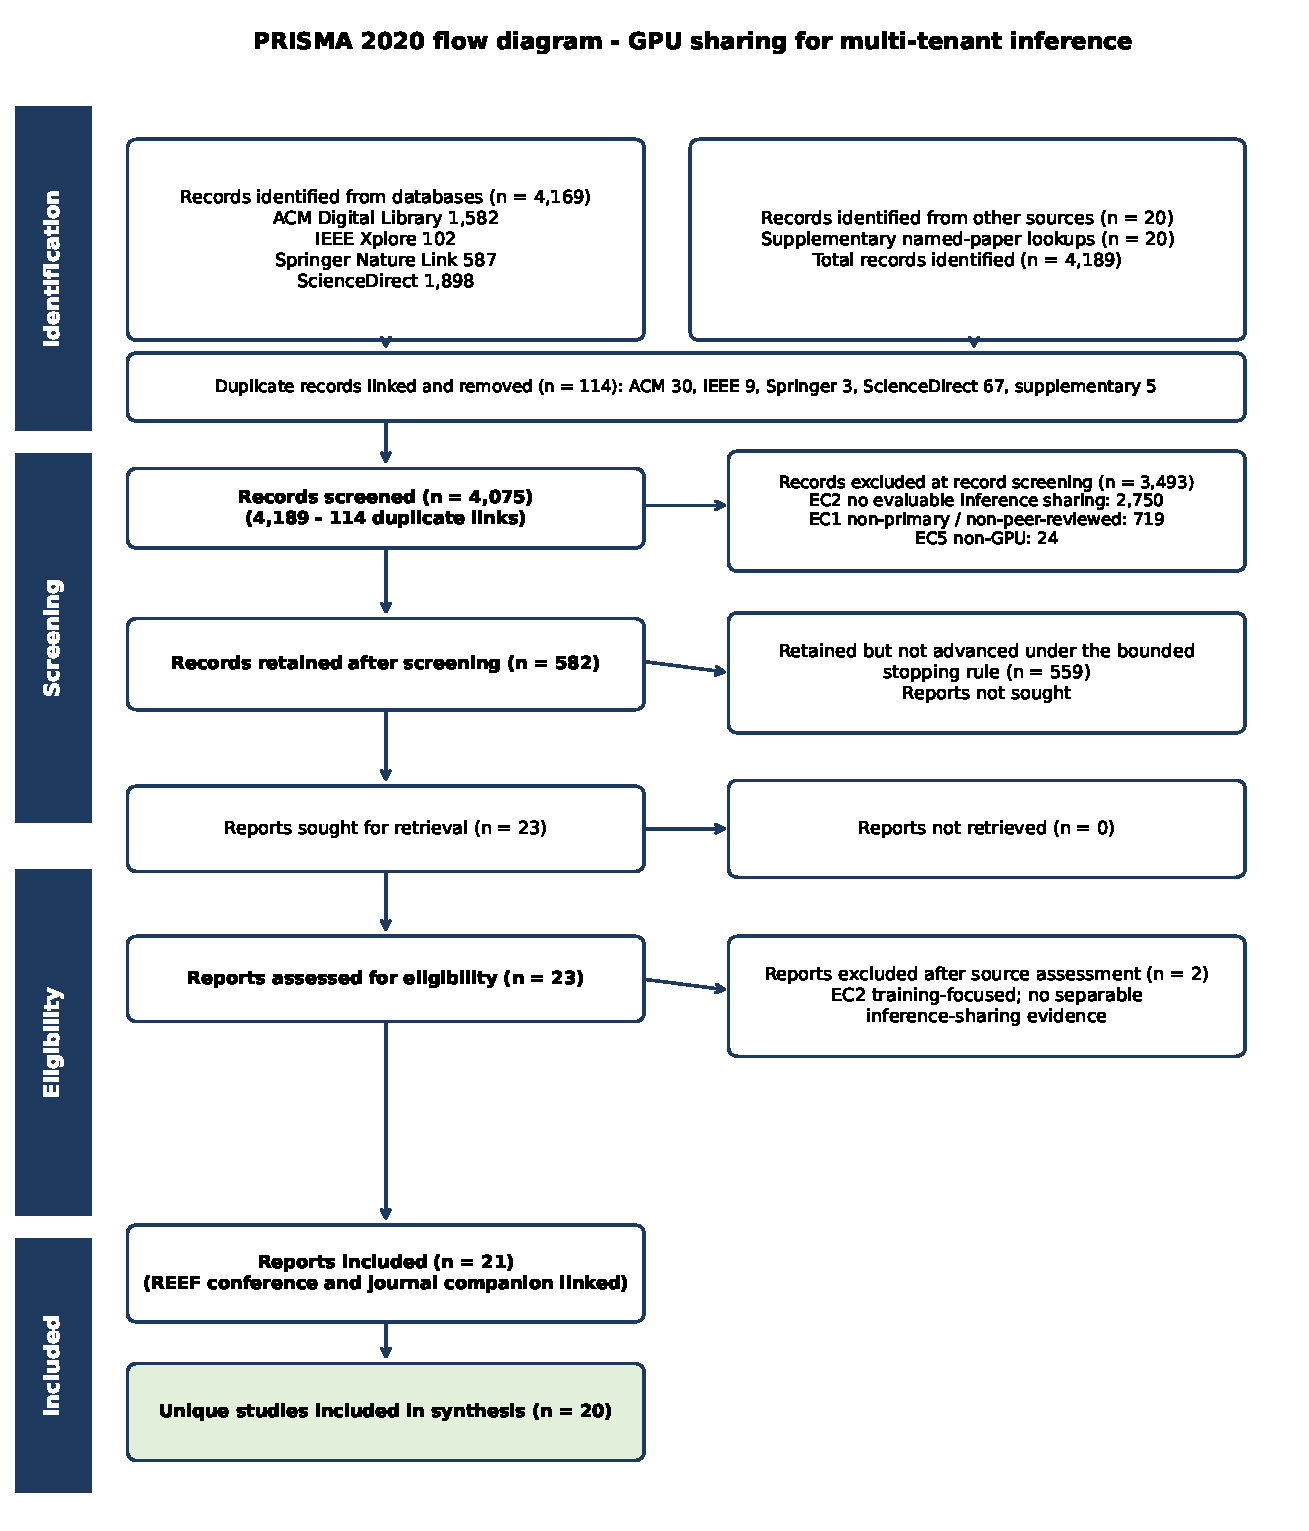
\includegraphics[width=\textwidth,height=.82\textheight,keepaspectratio]{../baseline/PRISMA_2020_FLOW_DIAGRAM.pdf}
\caption{Supplied bounded-review selection flow, preserved from Task 2. Current PDF download attempts are a separate activity.}
\end{figure}
\begin{longtable}{>{\raggedright\arraybackslash}p{0.16\textwidth}>{\raggedright\arraybackslash}p{0.62\textwidth}>{\raggedright\arraybackslash}p{0.1\textwidth}}
\toprule
\textbf{Study / report} & \textbf{System / source identity} & \textbf{QA}\\\midrule\endhead
S001 / P001 & VastPipe (2025) & 13/18\\\addlinespace
S002 / P002 & iGniter (2023) & 17/20\\\addlinespace
S003 / P003 & gpulets (2022) & 18/20\\\addlinespace
S004 / P004 & PipeSwitch (2020) & 17/20\\\addlinespace
S005 / P005 & REEF conference (2022) & 17/20\\\addlinespace
S006 / P006 & Paella: Low-latency Model Serving with Software-defined GPU Scheduling (2023) & 16/18\\\addlinespace
S007 / P007 & Orion: Interference-aware, Fine-grained GPU Sharing for ML Applications (2024) & 19/20\\\addlinespace
S008 / P008 & GSLICE: Controlled Spatial Sharing of GPUs for a Scalable Inference Platform (2020) & 17/20\\\addlinespace
S009 / P009 & Serving DNNs like Clockwork: Performance Predictability from the Bottom Up (2020) & 16/20\\\addlinespace
S010 / P010 & Colocating ML Inference and Training with Fast GPU Memory Handover (SIRIUS) (2025) & 17/20\\\addlinespace
S011 / P011 & ParvaGPU: Efficient Spatial GPU Sharing for Large-Scale DNN Inference in Cloud Environments (2024) & 14/20\\\addlinespace
S012 / P012 & Torpor: GPU-Enabled Serverless Computing for Low-Latency, Resource-Efficient Inference (2025) & 15/20\\\addlinespace
S013 / P013 & StreamBox: A Lightweight GPU SandBox for Serverless Inference Workflow (2024) & 15/20\\\addlinespace
S014 / P014 & Efficient Performance-Aware GPU Sharing with Compatibility and Isolation through Kernel Space Interception (KRYPTON) (2025) & 16/20\\\addlinespace
S015 / P015 & XSched: Preemptive Scheduling for Diverse XPUs (2025) & 16/18\\\addlinespace
S016 / P018 & InferFair: Towards QoS-aware scheduling for performance isolation guarantee in heterogeneous model serving systems (2024) & 15/20\\\addlinespace
S017 / P019 & ArkGPU: enabling applications' high-goodput co-location execution on multitasking GPUs (2023) & 16/20\\\addlinespace
S018 / P020 & Dyna-P: placement-aware dynamic partitioning for lightweight applications with modern GPUs (2025) & 15/20\\\addlinespace
S019 / P021 & KRISP: Enabling Kernel-wise RIght-sizing for Spatial Partitioned GPU Inference Servers (2023) & 16/20\\\addlinespace
S020 / P022 & Tally: Non-Intrusive Performance Isolation for Concurrent Deep Learning Workloads (2025) & 17/20\\\addlinespace
\bottomrule\end{longtable}

\section{Taxonomy of existing approaches}
A useful taxonomy separates the resource being controlled from the software layer implementing the policy. The same system may appear in more than one category. A MIG-based system can also use MPS; an API interceptor can enforce temporal scheduling; and memory handover can support mixed-workload co-location. Treating these as mutually exclusive labels would hide the source of the observed behavior.

\subsection{Temporal and priority control}
Temporal mechanisms decide which work runs and when another tenant can make progress. PipeSwitch emphasizes switching and model state, Clockwork emphasizes predictable execution and admission, while REEF, Paella, Orion and XSched expose different scheduling/preemption boundaries. Their integration costs and latency meanings differ. PipeSwitch's additional switching-related latency is not interchangeable with XSched's foreground P99 ratio or Paella's reported P99 reduction \cite{P004,P005,P006,P007,P009,P015}.

\subsection{Spatial allocation and partitions}
MPS-based allocation and software right-sizing regulate concurrent access to execution resources. VastPipe, iGniter, gpulets and GSLICE provide different allocation, profiling and feedback approaches. KRISP contributes AMD-oriented kernel right-sizing evidence and should not be relabeled as a measurement of NVIDIA MPS. Partition-aware designs, including ParvaGPU and Dyna-P, additionally make placement, profile size or reconfiguration relevant \cite{P001,P002,P003,P008,P011,P020,P021}.

A spatial allocation is only one part of a service guarantee. The model must fit memory, the workload must remain within the profiled regime and the selected resource shares must satisfy its timing requirements. Hardware allocation boundaries do not by themselves establish all possible security or fault guarantees in the reviewed experiments.

\subsection{API, runtime and memory mediation}
Torpor, StreamBox, KRYPTON, ArkGPU and Tally intervene at different points between the application and accelerator. Their common advantage is control over resource use without necessarily changing the model's high-level purpose. Their differences include intercepted interfaces, compatibility, runtime sharing, host work and the degree to which tenants share memory or trust assumptions. SIRIUS contributes a specific memory-handover mechanism for co-located inference and training \cite{P010,P012,P013,P014,P019,P022}.
\begin{longtable}{>{\raggedright\arraybackslash}p{0.25\textwidth}>{\raggedright\arraybackslash}p{0.35\textwidth}>{\raggedright\arraybackslash}p{0.28\textwidth}}
\toprule
\textbf{Family / reports} & \textbf{Control and condition} & \textbf{Cost}\\\midrule\endhead
Temporal / priority; P004 P005 P006 P007 P009 P015 P022 & Request, model, kernel or launch order. A suitable interception/preemption boundary exists & Switch cost, profiling and background slowdown\\\addlinespace
Software spatial sharing; P001 P002 P003 P008 P021 & MPS quota or AMD CU-mask control. Concurrent jobs fit memory and selected compute allocation & Residual interference; quotas are not proof of security\\\addlinespace
Hardware partition and hybrid; P011 P014 P020 & MIG profiles plus temporal/MPS policy. Supported partition profiles fit model memory & Fragmentation, placement and reconfiguration cost\\\addlinespace
API / runtime mediation; P006 P012 P013 P014 P019 P022 & User API, shared runtime or kernel interface. Required APIs and integration hooks are supported & Compatibility, CPU/transfer cost and trust boundary\\\addlinespace
Memory handover; P010 & Inference/training memory ownership. Training can yield memory without breaking inference & Reclamation and integration overhead\\\addlinespace
Fairness policy; P018 & Relative model slowdown and SLO goodput. Comparable per-model service objectives & Not equivalent to request-tail or hostile-tenant isolation\\\addlinespace
\bottomrule\end{longtable}

\section{Results and evidence synthesis by research question}
\subsection{RQ1: mechanisms and control boundaries}
The corpus supports a layered answer rather than a product list. Temporal control manages ordering and interruption; software spatial control manages concurrent allocation; hardware partitioning constrains resource placement; and API/runtime mediation supplies an enforcement layer. Fairness-aware policy adds a decision objective across these mechanisms. InferFair, for example, is best understood through relative slowdown and useful service, not as a new hardware partition primitive \cite{P018}.

This taxonomy explains why naming MPS, MIG or remoting is insufficient for engineering selection. A deployment also needs a policy, a mechanism for enforcing it and an explicit boundary of protection. The corpus demonstrates several combinations, but its bounded selection does not support a claim that one category is most prevalent in the entire literature.

\subsection{RQ2: measurements and comparability}
The outcome register includes requests/s, normalized throughput, goodput, P99/P98 latency, unspecified latency, SLO-violation rate, API overhead, host memory and a composite utilization-efficacy score. These measure different properties. Goodput counts work that meets a service objective, while aggregate throughput may include best-effort work that does not protect the foreground service. A numerical increase in the latter cannot establish improvement in the former.

GSLICE's GUE value of 94.04 is a composite score, not 94.04\% GPU utilization. Its negative signed latency improvement is retained as an unfavorable observation. The gpulets threshold covering 90\% of tested model pairs concerns a distribution across pairs, not the 90th percentile of requests. These distinctions prevent apparently precise but invalid conclusions \cite{P003,P008}.

The reported iGniter prediction-error range of 1.53--5.02\% assesses prediction accuracy, not a latency speedup. Clockwork's approximately 800 requests/s is goodput in a particular evaluation, and the supplied extraction notes a nonidentical comparator setup. Both observations are useful, but neither supports a direct ranking against a throughput ratio measured on another platform \cite{P002,P009}.

\subsection{RQ3: conditions affecting results}
Three conditions recur in the evidence. First, concurrency and resource shares affect both completed work and waiting time. The local ParvaGPU contrast shows a throughput benefit accompanied by increased latency. Second, model state and memory transfer can dominate. Torpor's late binding is attractive for low-rate functions, but its density result does not establish that frequent transfers of large models meet the same latency objective. Third, the workload's priority structure determines which sacrifice is acceptable \cite{P011,P012}.

For a foreground-priority service, XSched's 1.07x standalone P99 is relevant because it directly expresses foreground interference in the evaluated setup. Orion's up-to-7.3x aggregate-throughput result describes total work and must be read with its foreground-latency condition. These results can support different decisions without contradicting each other \cite{P007,P015}.

Mixed-workload evidence requires an additional separation. SIRIUS reports an average P99 inference improvement factor of 12.6 against the authors' adapted TaskSwitch baseline. It is not a uniform per-model gain or a direct comparison against unmodified PipeSwitch. ArkGPU's recorded inference/training pairs meet a twice-solo P99 target, while a low-contention setting can lose about 5\% QPS. The unfavorable condition belongs in the synthesis because it changes when the mechanism is worthwhile \cite{P010,P019}.

\subsection{RQ4: isolation and implementation cost}
Performance isolation asks whether another workload changes service behavior. Resource isolation asks what capacity is allocated or separated. Memory protection and fault containment concern different failure or adversarial models. A scheduler that limits slowdown is not thereby a complete hostile-tenant security boundary. The extraction cards preserve these dimensions separately, and untested boundaries remain unestablished.

Implementation costs also operate at different levels. API mediation can add host-side work or per-call delay. Model swapping adds transfer and memory pressure. Kernel-space interception introduces compatibility and maintenance requirements. Temporal granularity changes the trade-off between scheduling work and waiting time. The KRYPTON extraction reports an average QoS violation rate of 1.23\% relative to a solo P99 threshold, which is a threshold-relative request fraction rather than a latency in milliseconds. Its original Poisson rate is half the solo maximum; the shared test halves that rate again while assigning 50\% time \cite{P014}.

\subsection{RQ5: conditional selection}
The evidence supports a sequence of decisions. Specify the service objective and trust boundary first. Eliminate mechanisms incompatible with hardware, model memory or required integration. Compare the remaining candidates under the relevant arrival process, batch and co-tenant mix. Measure both protected service and work sacrificed. If the available studies do not cover the required boundary, the appropriate conclusion is insufficient evidence for that guarantee, not an assumed benefit.

The recommendation matrix in Section~10 connects each scenario to report IDs, expected benefits, costs and alternatives. These are evidence-supported candidates for evaluation, not claims that the reviewed implementation can be deployed unchanged in every environment.

\section{Comparative analysis}
The comparison distinguishes direct within-source contrasts from unmatched cross-study observations. The strongest numerical statements are tied to their original comparator. Even these require attention to whether the result is an average, maximum, lower bound or threshold-relative statistic. An improvement described as ``up to'' is not the expected result for an arbitrary deployment.

\begin{longtable}{>{\raggedright\arraybackslash}p{0.26\textwidth}>{\raggedright\arraybackslash}p{0.28\textwidth}>{\raggedright\arraybackslash}p{0.34\textwidth}}
\toprule
\textbf{Evidence / class} & \textbf{Observation} & \textbf{Interpretation and missing control}\\\midrule\endhead
CMP01 P011 E036 E037 C001 C002. Within-source trade-off & 354 to 446 requests/s; 11 to 27 ms & 25.99\% throughput increase accompanies 2.4545x latency. Missing: Latency quantile; final version equivalence\\\addlinespace
CMP02 P001 E001; P011 E036. Unmatched cross-study & 2.7x versus 25.99\% increase & Different baseline and GPU/model context prevent ranking. Missing: Matched workload, batch and resource budget\\\addlinespace
CMP03 P007 E029 E030; P015 E044. Different objectives & Up to 7.3x aggregate work versus 1.07x foreground P99 & Foreground delay and total completed work must be assessed together. Missing: Common model mix and background progress metric\\\addlinespace
CMP04 P008 E031 E032. Within-source metric tension & GUE 94.04 and negative signed latency improvement & Composite efficacy is not utilization percent; preserve adverse latency. Missing: Metric definitions and baseline stratum\\\addlinespace
CMP05 P012 E038 E039. Condition-dependent trade-off & Density benefit with model-transfer sensitivity & Late binding suits low-rate functions only if transfer fits SLO. Missing: Heavy-model transfer and host CPU budget\\\addlinespace
CMP06 P019 E048 E049; P022 E052. Different experiments, consistent cost & QoS protection with low-contention or background throughput loss & Protecting foreground work can sacrifice co-tenant work. Missing: Matched slowdown definitions\\\addlinespace
CMP07 P005 P023. Companion study, not replication & REEF engines and report versions differ & Retain source-version strata; do not double-count corroboration. Missing: Outcome-to-version mapping for every combined REEF row\\\addlinespace
CMP08 P018 E046 E047; P020 E050. Different metrics & Goodput/fairness versus makespan & Job-level efficiency cannot establish request-tail service. Missing: Request arrival process and latency distribution\\\addlinespace
\bottomrule\end{longtable}

The evidence table in Appendix~\ref{app:evidence} retains all 52 supplied observations. The comparative matrix is deliberately smaller because its role is to explain a decision, not duplicate the extraction register. A claim can be traced from a recommendation to a report, then to an outcome ID and its page/figure anchor. Where a comparison remains unmatched, the matrix names the missing control rather than calculating a misleading combined effect.

\section{Engineering trade-off analysis}
\subsection{Utilization versus latency}
Additional concurrency is beneficial only while useful service increases under the required latency objective. The ParvaGPU example changes throughput by
\[ (446/354-1)\times100 = 25.99\%, \]
while latency changes by
\[ 27/11 = 2.4545. \]
These are calculations from recorded inputs, not newly measured outcomes. A service with a tight delay budget might reject this configuration despite its higher throughput. Another service might accept it if the increased latency remains within its own budget. Because the source quantile is unspecified, neither interpretation establishes P99 compliance \cite{P011}.

\subsection{Foreground protection versus background progress}
Priority is an allocation choice. Tally's supplied contrast records normalized background throughput of 1.19 versus 1.65 for TGS at the stated idle-time setting. This does not make foreground protection ineffective; it identifies the work sacrificed. Similarly, an aggregate-throughput gain must not hide deterioration in the protected request class. The engineering evaluation should report foreground latency and background progress together \cite{P022}.

\subsection{Memory density versus transfer and trust costs}
Shared runtimes and late binding can allow more functions or models to use limited GPU memory. StreamBox's workflow-oriented sharing and Torpor's binding decisions address this problem from different directions. Their density gains cannot be separated from concurrency, model-loading and trust assumptions. When large models are invoked frequently, transfer demand can undermine the benefit of keeping fewer models resident. When functions require stronger separation, a shared runtime may not provide the required boundary. Torpor explicitly distinguishes runtime-sharing evaluation from runtime-isolation deployment, and describes restart/migration recovery; these design claims are not direct fault-injection results \cite{P012,P013}.

\subsection{Partition control versus flexibility}
Hardware profiles constrain placement and memory fit. Software policies can improve use of a chosen profile, but fine-grained application demand need not align with fixed partitions. Dyna-P's recorded sensitivity to prediction perturbation concerns makespan, while online serving additionally needs evidence about individual request delays. The review therefore treats placement efficiency as relevant but insufficient evidence for latency-sensitive request serving \cite{P020}.

\section{Discussion and conflicting evidence}
\subsection{Apparent conflicts versus controlled disagreements}
A valid conflicting-evidence analysis first asks whether two studies measure the same quantity under comparable conditions. VastPipe's 2.7x throughput contrast and the calculated 25.99\% ParvaGPU increase have different baselines and workloads. Their unequal magnitudes do not show disagreement. Likewise, Orion's aggregate throughput, SIRIUS's average P99 improvement and XSched's normalized foreground P99 do not compete on a common scale \cite{P001,P007,P010,P011,P015}.

More useful tensions occur inside an experiment: improved throughput accompanied by higher latency, or protection of foreground work accompanied by lower background progress. The negative GSLICE latency contrast and ArkGPU's low-contention regression show conditions in which a favorable overall mechanism narrative is incomplete. These observations constrain applicability rather than being dismissed as exceptions \cite{P008,P019}.

\subsection{Version and engine effects}
The REEF journal extension adds implementation and evaluation beyond the conference report. The supplied extraction already distinguishes PyTorch and TensorRT conditions in its discussion. Combining all favorable points into one synthetic result would obscure both the engine difference and the report-version difference. The current study-level mapping avoids double-counting, but each combined REEF outcome still needs an explicit conference-versus-journal source assignment before final submission \cite{P005,P023}.

\subsection{Strength of the engineering argument}
The repeated pattern is that resource sharing works through a mechanism-specific constraint: interruption cost, quota fit, memory residency, partition placement or compatibility. This pattern supports conditional design reasoning. It does not establish identical effect sizes or a common security guarantee across systems. The draft's recommendations remain narrower than a claim of deployment readiness.

\section{Evidence-based engineering recommendations}
\subsubsection*{REC01: Trusted resident models; utilization priority}
\begin{longtable}{>{\raggedright\arraybackslash}p{0.22\textwidth}>{\raggedright\arraybackslash}p{0.7\textwidth}}
\toprule
\textbf{Dimension} & \textbf{Assessment}\\\midrule\endhead
Candidate & Tuned MPS / software spatial controls\\\addlinespace
Evidence & P001 P002 P003 P008 E001-E004 E006 E031-E032\\\addlinespace
Expected benefit & Higher useful co-location under tested allocations\\\addlinespace
Sacrifice & Interference, quota tuning and memory pressure\\\addlinespace
Alternative / trigger & Partitions or dedication when trust/isolation dominates\\\addlinespace
Validation needed & Measure each model P99 and SLO goodput under bursts\\\addlinespace
\bottomrule\end{longtable}
\subsubsection*{REC02: Foreground tail-latency priority}
\begin{longtable}{>{\raggedright\arraybackslash}p{0.22\textwidth}>{\raggedright\arraybackslash}p{0.7\textwidth}}
\toprule
\textbf{Dimension} & \textbf{Assessment}\\\midrule\endhead
Candidate & Priority/preemptive scheduling\\\addlinespace
Evidence & P005 P006 P007 P015 P022 E018-E030 E044-E045 E052\\\addlinespace
Expected benefit & Lower foreground interference\\\addlinespace
Sacrifice & Background slowdown, profiling and runtime integration\\\addlinespace
Alternative / trigger & Dedicated GPU when supported control cannot meet deadline\\\addlinespace
Validation needed & Check foreground tails and background progress jointly\\\addlinespace
\bottomrule\end{longtable}
\subsubsection*{REC03: Low-rate serverless functions}
\begin{longtable}{>{\raggedright\arraybackslash}p{0.22\textwidth}>{\raggedright\arraybackslash}p{0.7\textwidth}}
\toprule
\textbf{Dimension} & \textbf{Assessment}\\\midrule\endhead
Candidate & Late binding / controlled runtime sharing\\\addlinespace
Evidence & P012 P013 E038-E041\\\addlinespace
Expected benefit & Higher function or workflow density\\\addlinespace
Sacrifice & Host CPU, memory transfer and shared-runtime trust\\\addlinespace
Alternative / trigger & Keep large or high-rate models resident if swaps dominate\\\addlinespace
Validation needed & Sweep model sizes, cold starts, offered rate and concurrency\\\addlinespace
\bottomrule\end{longtable}
\subsubsection*{REC04: Mixed inference with opportunistic training}
\begin{longtable}{>{\raggedright\arraybackslash}p{0.22\textwidth}>{\raggedright\arraybackslash}p{0.7\textwidth}}
\toprule
\textbf{Dimension} & \textbf{Assessment}\\\midrule\endhead
Candidate & Memory handover / controlled co-location\\\addlinespace
Evidence & P010 P019 E035 E048-E049\\\addlinespace
Expected benefit & Protect inference while using residual capacity\\\addlinespace
Sacrifice & Reclamation overhead and reduced training progress\\\addlinespace
Alternative / trigger & Separate resources for intolerable interference\\\addlinespace
Validation needed & Measure inference tails separately from training throughput\\\addlinespace
\bottomrule\end{longtable}
\subsubsection*{REC05: Supported partition hardware; stable memory fit}
\begin{longtable}{>{\raggedright\arraybackslash}p{0.22\textwidth}>{\raggedright\arraybackslash}p{0.7\textwidth}}
\toprule
\textbf{Dimension} & \textbf{Assessment}\\\midrule\endhead
Candidate & MIG-aware hybrid policy\\\addlinespace
Evidence & P011 P014 P020 E036-E037 E042-E043 E050\\\addlinespace
Expected benefit & Resource allocation with configurable co-location\\\addlinespace
Sacrifice & Fragmentation and reconfiguration overhead\\\addlinespace
Alternative / trigger & Software sharing when partition granularity wastes capacity\\\addlinespace
Validation needed & Validate profile fit and reconfiguration effects; security needs separate tests\\\addlinespace
\bottomrule\end{longtable}
\subsubsection*{REC06: Several models with unequal service pressure}
\begin{longtable}{>{\raggedright\arraybackslash}p{0.22\textwidth}>{\raggedright\arraybackslash}p{0.7\textwidth}}
\toprule
\textbf{Dimension} & \textbf{Assessment}\\\midrule\endhead
Candidate & Fairness-aware admission / scheduling\\\addlinespace
Evidence & P018 E046-E047\\\addlinespace
Expected benefit & Balance normalized slowdown and SLO goodput\\\addlinespace
Sacrifice & May give up aggregate throughput to improve fairness\\\addlinespace
Alternative / trigger & Priority scheduling when one foreground SLA dominates\\\addlinespace
Validation needed & Agree fairness objective and per-model SLO before deployment\\\addlinespace
\bottomrule\end{longtable}
The recommended deployment assessment begins with the actual service objective: per-model deadline or percentile target, admissible violation rate and minimum background progress. These values must come from the intended deployment rather than being invented from a paper. The next step is a local comparison using the same model versions, input sizes, batching and offered load. Cold starts and bursts should be retained if they occur in the application.

A candidate is suitable only if it meets the required service objective at an acceptable cost. The acceptance evidence should include per-tenant latency, SLO-compliant goodput, memory pressure, resource utilization with a defined instrument, host overhead and the relevant isolation tests. The review supplies a shortlist and the reasons to test it; it does not supply a universal numerical threshold or imply that a benchmark result transfers unchanged.

\section{Research gaps and future directions}
\begin{longtable}{>{\raggedright\arraybackslash}p{0.28\textwidth}>{\raggedright\arraybackslash}p{0.22\textwidth}>{\raggedright\arraybackslash}p{0.38\textwidth}}
\toprule
\textbf{Corpus gap} & \textbf{Basis} & \textbf{Next experiment}\\\midrule\endhead
No matched all-family comparison & Comparability CMP01-CMP08 & Same GPU, model mix, memory budget, arrivals and SLO across families\\\addlinespace
Security/fault boundaries often unestablished & Extraction Security boundary / Fault boundary & Separate adversarial access, fault injection and performance tests\\\addlinespace
Metrics emphasize different units & E001-E052 & Report per-model goodput, tails and background progress jointly\\\addlinespace
Partition prediction affects makespan & P020 E050 & Bursty arrivals plus placement changes and request-tail measurement\\\addlinespace
Version and method details remain incomplete & P002 P011 P022; QA Q3/Q4/Q10 & Publish exact version, driver/runtime, warmup, repetitions and uncertainty\\\addlinespace
Energy and cost evidence not harmonized & Extraction schema and heterogeneous outcomes & Measure GPU and host energy per SLO-compliant request\\\addlinespace
\bottomrule\end{longtable}
These gaps are observations about this corpus and its reporting, not assertions that no relevant research exists anywhere. The 559-record unassessed branch makes that distinction essential. A stronger future comparison would align hardware, workload, baselines and outcome definitions across mechanism families, then report both benefits and sacrifices. Energy per useful request and failure/security behavior require separate measurements rather than extrapolation from utilization.

\section{Threats to validity and limitations}
\begin{longtable}{>{\raggedright\arraybackslash}p{0.32\textwidth}>{\raggedright\arraybackslash}p{0.26\textwidth}>{\raggedright\arraybackslash}p{0.3\textwidth}}
\toprule
\textbf{Threat / consequence} & \textbf{Mitigation} & \textbf{Remaining work}\\\midrule\endhead
Selection/stopping: No exhaustive recall or prevalence claim & Stopping branch remains visible & Instructor/team decision on bounded scope; extend if required\\\addlinespace
Title-only decisions: Relevant work may be missed & Abstract-availability column retained & Prioritize uncertain/relevant records for abstract checks\\\addlinespace
Single review: Correlated screening/QA/extraction errors possible & Original rationale and source anchors retained & Record real named checks if performed\\\addlinespace
Search provenance: Search cannot be fully reconstructed from totals & Exact preserved query/log values retained & Supply missing original exports, facets and receipts\\\addlinespace
Source version: Page/result mappings may differ & Separate source-version and retrieval records & Compare final published text and map companion outcomes\\\addlinespace
Measurement heterogeneity: Cross-study speedup ranking is invalid & No pooled effect size or universal winner & Matched comparisons needed\\\addlinespace
Reporting bias: Headlines may overstate robustness & Adverse and null findings retained & Recheck high-impact claims at exact source locations\\\addlinespace
\bottomrule\end{longtable}
The most material limitation is selection: a bounded source set cannot establish exhaustive coverage. The large number of title-only records compounds that risk. The single-assessment method creates a separate risk of correlated errors even where spreadsheet arithmetic is correct. Finally, retrieved author manuscripts may differ from the version used by the original extraction, and access to a PDF does not constitute verification of every result.

Mitigations in this draft include immutable baseline files, separate current retrieval records, stable IDs, preserved unfavorable findings, explicit source/version limits and no numerical pooling across unmatched studies. These measures improve traceability but do not erase the underlying limitations. Final acceptance requires resolving the scope decision and recording any actual independent checks at the item level.

\section{Conclusion}
The bounded 20-study corpus supports a conditional approach to GPU sharing for multi-tenant inference. Temporal control is relevant when foreground response dominates; software spatial sharing is relevant when trusted co-location can exploit spare capacity; partition-aware designs make resource fit and reconfiguration central; and runtime or memory mediation can increase density at a transfer, integration or trust cost. Each choice must be evaluated against its own baseline and intended conditions.

The principal outcome is therefore a traceable selection framework, not a universal ranking. The first draft covers the instructor's analytical requirements through Section 22 and follows the suggested final-report sequence. It remains a draft: the bounded scope, source-version mappings, incomplete PDF collection and item-level checking require explicit closure before the work is represented as a fully verified final SLR.

\clearpage\bibliographystyle{ieeetr}\bibliography{references}
\clearpage\appendix\section{Exact search register}\label{app:search}

The following entries are preserved from the supplied workbook. Date precision, provenance and count discrepancies remain as recorded.

\subsection{IEEE-MPS}

\begin{longtable}{>{\raggedright\arraybackslash}p{0.25\textwidth}>{\raggedright\arraybackslash}p{0.65\textwidth}}
\toprule
\textbf{Field} & \textbf{Recorded value}\\\midrule\endhead
Platform & IEEE Xplore\\\addlinespace
Status & executed search record preserved in the project register\\\addlinespace
Exact query & (GPU OR "graphics processing unit") AND (inference OR "model serving" OR "deep learning" OR DNN OR LLM) AND (MPS OR "multi-process service")\\\addlinespace
Fields & All metadata (Search by All); not field-qualified Command Search\\\addlinespace
Filters & Publication years2020-2026; date/language/type checked during screening\\\addlinespace
Recorded search date / time & 2026-10-11\\\addlinespace
Displayed hits & 25\\\addlinespace
Exported records & 25\\\addlinespace
Parsed records & 25\\\addlinespace
Active records & 25\\\addlinespace
Files & \nolinkurl{https://github.com/Raazia-Imran/os_CEPPPPPP/blob/main/evidence/imports/group-a/imported_records.json}\\\addlinespace
Notes & Rendered metadata capture, not publisher export; exact time unavailable; different expressions from submitted protocol; full text indexed scope for Springer\\\addlinespace
Provenance & Group A run, reused (counts identical to Group A report, 16 Oct 2026)\\\addlinespace
\bottomrule\end{longtable}

\subsection{IEEE-MIG}

\begin{longtable}{>{\raggedright\arraybackslash}p{0.25\textwidth}>{\raggedright\arraybackslash}p{0.65\textwidth}}
\toprule
\textbf{Field} & \textbf{Recorded value}\\\midrule\endhead
Platform & IEEE Xplore\\\addlinespace
Status & executed search record preserved in the project register\\\addlinespace
Exact query & (GPU OR "graphics processing unit") AND (inference OR "model serving" OR "deep learning" OR DNN OR LLM) AND (MIG OR "multi-instance GPU" OR "GPU partitioning")\\\addlinespace
Fields & All metadata (Search by All); not field-qualified Command Search\\\addlinespace
Filters & Publication years2020-2026; date/language/type checked during screening\\\addlinespace
Recorded search date / time & 2026-10-11\\\addlinespace
Displayed hits & 23\\\addlinespace
Exported records & 23\\\addlinespace
Parsed records & 23\\\addlinespace
Active records & 23\\\addlinespace
Files & \nolinkurl{https://github.com/Raazia-Imran/os_CEPPPPPP/blob/main/evidence/imports/group-a/imported_records.json}\\\addlinespace
Notes & Rendered metadata capture, not publisher export; exact time unavailable; different expressions from submitted protocol; full text indexed scope for Springer\\\addlinespace
Provenance & Group A run, reused (counts identical to Group A report, 16 Oct 2026)\\\addlinespace
\bottomrule\end{longtable}

\subsection{IEEE-TEMPORAL}

\begin{longtable}{>{\raggedright\arraybackslash}p{0.25\textwidth}>{\raggedright\arraybackslash}p{0.65\textwidth}}
\toprule
\textbf{Field} & \textbf{Recorded value}\\\midrule\endhead
Platform & IEEE Xplore\\\addlinespace
Status & executed search record preserved in the project register\\\addlinespace
Exact query & (GPU OR "graphics processing unit") AND (inference OR "model serving" OR "deep learning" OR DNN OR LLM) AND ("time slicing" OR "time sharing" OR "context switching")\\\addlinespace
Fields & All metadata (Search by All); not field-qualified Command Search\\\addlinespace
Filters & Publication years2020-2026; date/language/type checked during screening\\\addlinespace
Recorded search date / time & 2026-10-11\\\addlinespace
Displayed hits & 45\\\addlinespace
Exported records & 45\\\addlinespace
Parsed records & 45\\\addlinespace
Active records & 45\\\addlinespace
Files & \nolinkurl{https://github.com/Raazia-Imran/os_CEPPPPPP/blob/main/evidence/imports/group-a/imported_records.json}\\\addlinespace
Notes & Rendered metadata capture, not publisher export; exact time unavailable; different expressions from submitted protocol; full text indexed scope for Springer\\\addlinespace
Provenance & Group A run, reused (counts identical to Group A report, 16 Oct 2026)\\\addlinespace
\bottomrule\end{longtable}

\subsection{IEEE-API}

\begin{longtable}{>{\raggedright\arraybackslash}p{0.25\textwidth}>{\raggedright\arraybackslash}p{0.65\textwidth}}
\toprule
\textbf{Field} & \textbf{Recorded value}\\\midrule\endhead
Platform & IEEE Xplore\\\addlinespace
Status & executed search record preserved in the project register\\\addlinespace
Exact query & (GPU OR "graphics processing unit") AND (inference OR "model serving" OR "deep learning" OR DNN OR LLM) AND ("API remoting" OR "CUDA remoting" OR "GPU proxy" OR "GPU virtualization")\\\addlinespace
Fields & All metadata (Search by All); not field-qualified Command Search\\\addlinespace
Filters & Publication years2020-2026; date/language/type checked during screening\\\addlinespace
Recorded search date / time & 2026-10-11\\\addlinespace
Displayed hits & 9\\\addlinespace
Exported records & 9\\\addlinespace
Parsed records & 9\\\addlinespace
Active records & 9\\\addlinespace
Files & \nolinkurl{https://github.com/Raazia-Imran/os_CEPPPPPP/blob/main/evidence/imports/group-a/imported_records.json}\\\addlinespace
Notes & Rendered metadata capture, not publisher export; exact time unavailable; different expressions from submitted protocol; full text indexed scope for Springer\\\addlinespace
Provenance & Group A run, reused (counts identical to Group A report, 16 Oct 2026)\\\addlinespace
\bottomrule\end{longtable}

\subsection{SPR-MASTER}

\begin{longtable}{>{\raggedright\arraybackslash}p{0.25\textwidth}>{\raggedright\arraybackslash}p{0.65\textwidth}}
\toprule
\textbf{Field} & \textbf{Recorded value}\\\midrule\endhead
Platform & Springer Nature Link\\\addlinespace
Status & executed search record preserved in the project register\\\addlinespace
Exact query & (GPU OR "graphics processing unit") AND (inference OR "model serving" OR "deep learning" OR DNN OR LLM) AND ("time slicing" OR "time sharing" OR "context switching" OR MPS OR "multi-process service" OR MIG OR "multi-instance GPU" OR "GPU partitioning" OR "API remoting" OR "CUDA remoting" OR "GPU proxy" OR "GPU virtualization")\\\addlinespace
Fields & General search/full-text indexed collection\\\addlinespace
Filters & English; Research article OR Conference paper;2020-2026; manual cutoff\\\addlinespace
Recorded search date / time & 2026-10-11\\\addlinespace
Displayed hits & 587\\\addlinespace
Exported records & 587\\\addlinespace
Parsed records & 587\\\addlinespace
Active records & 587\\\addlinespace
Files & \nolinkurl{https://github.com/Raazia-Imran/os_CEPPPPPP/blob/main/evidence/imports/group-a/imported_records.json}\\\addlinespace
Notes & Rendered metadata capture, not publisher export; exact time unavailable; different expressions from submitted protocol; full text indexed scope for Springer\\\addlinespace
Provenance & Group A run, reused (counts identical to Group A report, 16 Oct 2026)\\\addlinespace
\bottomrule\end{longtable}

\subsection{ACM-PILOT}

\begin{longtable}{>{\raggedright\arraybackslash}p{0.25\textwidth}>{\raggedright\arraybackslash}p{0.65\textwidth}}
\toprule
\textbf{Field} & \textbf{Recorded value}\\\midrule\endhead
Platform & ACM Digital Library\\\addlinespace
Status & Blocked pilot; no records imported\\\addlinespace
Exact query & GPU AND inference AND MPS\\\addlinespace
Fields & not\_validated\\\addlinespace
Filters & not\_applied\\\addlinespace
Recorded search date / time & 2026-10-11\\\addlinespace
Displayed hits & UNKNOWN\\\addlinespace
Exported records & 0\\\addlinespace
Parsed records & 0\\\addlinespace
Active records & 0\\\addlinespace
Files & supplied search \nolinkurl{export/imported_records.json}\\\addlinespace
Notes & Rendered metadata capture, not publisher export; exact time unavailable; different expressions from submitted protocol; full text indexed scope for Springer\\\addlinespace
Provenance & Pilot checkpoint of 11 Oct 2026 (search blocked/unavailable; no import), as in Group A report\\\addlinespace
\bottomrule\end{longtable}

\subsection{SD-PILOT}

\begin{longtable}{>{\raggedright\arraybackslash}p{0.25\textwidth}>{\raggedright\arraybackslash}p{0.65\textwidth}}
\toprule
\textbf{Field} & \textbf{Recorded value}\\\midrule\endhead
Platform & ScienceDirect\\\addlinespace
Status & Blocked pilot; no records imported\\\addlinespace
Exact query & GPU AND inference AND MPS\\\addlinespace
Fields & not\_validated\\\addlinespace
Filters & not\_applied\\\addlinespace
Recorded search date / time & 2026-10-11\\\addlinespace
Displayed hits & UNKNOWN\\\addlinespace
Exported records & 0\\\addlinespace
Parsed records & 0\\\addlinespace
Active records & 0\\\addlinespace
Files & supplied search \nolinkurl{export/imported_records.json}\\\addlinespace
Notes & Rendered metadata capture, not publisher export; exact time unavailable; different expressions from submitted protocol; full text indexed scope for Springer\\\addlinespace
Provenance & Pilot checkpoint of 11 Oct 2026 (search blocked/unavailable; no import), as in Group A report\\\addlinespace
\bottomrule\end{longtable}

\subsection{SUP-SELECTED}

\begin{longtable}{>{\raggedright\arraybackslash}p{0.25\textwidth}>{\raggedright\arraybackslash}p{0.65\textwidth}}
\toprule
\textbf{Field} & \textbf{Recorded value}\\\midrule\endhead
Platform & Supplementary public web/venue/author lookup\\\addlinespace
Status & executed search record preserved in the project register\\\addlinespace
Exact query & Named-paper lookups and official venue/author retrieval; see \nolinkurl{supplementary_discovery.csv}\\\addlinespace
Fields & Public metadata/full texts\\\addlinespace
Filters & Same protocol eligibility\\\addlinespace
Recorded search date / time & 2026-10-11\\\addlinespace
Displayed hits & UNKNOWN\\\addlinespace
Exported records & 20\\\addlinespace
Parsed records & 20\\\addlinespace
Active records & 20\\\addlinespace
Files & \nolinkurl{evidence/imports/group-a/supplementary_discovery.csv}\\\addlinespace
Notes & 20 selected named-paper records in the preserved source register; this is not an exhaustive web search. Query wording is a reproducible follow-up, not a verbatim historical query.\\\addlinespace
Provenance & Shared original-collector register, retained with its source IDs; no new search claimed.\\\addlinespace
\bottomrule\end{longtable}

\subsection{ACM-MASTER}

\begin{longtable}{>{\raggedright\arraybackslash}p{0.25\textwidth}>{\raggedright\arraybackslash}p{0.65\textwidth}}
\toprule
\textbf{Field} & \textbf{Recorded value}\\\midrule\endhead
Platform & ACM Digital Library\\\addlinespace
Status & reported master query; master and numbered exports not fully mapped\\\addlinespace
Exact query & (GPU OR "graphics processing unit") AND (inference OR "model serving" OR "deep learning" OR DNN OR LLM) AND ("time slicing" OR "time sharing" OR "context switching" OR MPS OR "multi-process service" OR MIG OR "multi-instance GPU" OR "GPU partitioning" OR "API remoting" OR "CUDA remoting" OR "GPU proxy" OR "GPU virtualization")\\\addlinespace
Fields & All Fields\\\addlinespace
Filters & 2020 - 2026\\\addlinespace
Recorded search date / time & 2026-10-14 22:30 PKT (UTC+05:00; operator-reported)\\\addlinespace
Displayed hits & 1600\\\addlinespace
Exported records & 1603\\\addlinespace
Parsed records & 1829\\\addlinespace
Active records & 0\\\addlinespace
Files & \nolinkurl{evidence/incoming_shared/acm_master/ACM_MASTER_01.bib;evidence/incoming_shared/acm_master/ACM_MASTER_02.bib}\\\addlinespace
Notes & Separate master exports contain 1,829 overlapping occurrences / 1,387 distinct DOI-or-title keys. Reported displayed 1,600 and claimed export 1,603 do not reproduce those bytes. Active contribution is zero; do not assign the 1,582 numbered occurrences to this run without mapping evidence. Source: \nolinkurl{evidence/incoming_shared/acm_master/reconciliation.json.}\\\addlinespace
Provenance & Historical operator-reported run; timestamp/query from \nolinkurl{evidence/incoming_shared/search_log_2026-10-16.txt;} not independently rerun.\\\addlinespace
\bottomrule\end{longtable}

\subsection{SD-TEMPORAL}

\begin{longtable}{>{\raggedright\arraybackslash}p{0.25\textwidth}>{\raggedright\arraybackslash}p{0.65\textwidth}}
\toprule
\textbf{Field} & \textbf{Recorded value}\\\midrule\endhead
Platform & ScienceDirect\\\addlinespace
Status & historical operator-reported; partial export reconciliation\\\addlinespace
Exact query & (GPU OR "graphics processing unit") AND (inference OR "model serving" OR "deep learning") AND ("time slicing" OR "time sharing" OR "context switching")\\\addlinespace
Fields & Find articles with these terms\\\addlinespace
Filters & 2020-2026; supplied URL explicitly includes accessTypes=openaccess (not stated in original filter text).\\\addlinespace
Recorded search date / time & 2026-10-14 23:45 PKT (UTC+05:00; operator-reported)\\\addlinespace
Displayed hits & 1053\\\addlinespace
Exported records & 1053\\\addlinespace
Parsed records & 1053\\\addlinespace
Active records & 1053\\\addlinespace
Files & \nolinkurl{evidence/incoming_shared/sciencedirect_2026-10-16/SD_TEMPORAL_01.ris;evidence/incoming_shared/sciencedirect_2026-10-16/SD_TEMPORAL_010.ris;evidence/incoming_shared/sciencedirect_2026-10-16/SD_TEMPORAL_011.ris;evidence/incoming_shared/sciencedirect_2026-10-16/SD_TEMPORAL_02.ris;evidence/incoming_shared/sciencedirect_2026-10-16/SD_TEMPORAL_03.ris;evidence/incoming_shared/sciencedirect_2026-10-16/SD_TEMPORAL_04.ris;evidence/incoming_shared/sciencedirect_2026-10-16/SD_TEMPORAL_05.ris;evidence/incoming_shared/sciencedirect_2026-10-16/SD_TEMPORAL_06.ris;evidence/incoming_shared/sciencedirect_2026-10-16/SD_TEMPORAL_07.ris;evidence/incoming_shared/sciencedirect_2026-10-16/SD_TEMPORAL_08.ris;evidence/incoming_shared/sciencedirect_2026-10-16/SD_TEMPORAL_09.ris}\\\addlinespace
Notes & TEMPORAL URL has openaccess facet omitted from filter text; 1053 parsed agrees with reported count; exact pagination and operator unknown Repository check: standalone \nolinkurl{evidence/incoming_shared/SD_TEMPORAL_01(1).ris} contains 25 records only; it is not the 1053-occurrence full TEMPORAL archive cited in the project register. Later archive files are not present in the inspected remote tree. Original reported/registered counts are preserved, not revalidated from this sample.\\\addlinespace
Provenance & Historical operator-reported run; timestamp/query from \nolinkurl{evidence/incoming_shared/search_log_2026-10-16.txt;} not independently rerun.\\\addlinespace
\bottomrule\end{longtable}

\subsection{SD-MPS}

\begin{longtable}{>{\raggedright\arraybackslash}p{0.25\textwidth}>{\raggedright\arraybackslash}p{0.65\textwidth}}
\toprule
\textbf{Field} & \textbf{Recorded value}\\\midrule\endhead
Platform & ScienceDirect\\\addlinespace
Status & historical operator-reported; partial export reconciliation\\\addlinespace
Exact query & (GPU OR "graphics processing unit") AND (inference OR "model serving" OR "deep learning") AND (MPS OR "multi-process service")\\\addlinespace
Fields & Find articles with these terms\\\addlinespace
Filters & 2020 - 2026\\\addlinespace
Recorded search date / time & 2026-10-14 23:52 PKT (UTC+05:00; operator-reported)\\\addlinespace
Displayed hits & 517\\\addlinespace
Exported records & 563\\\addlinespace
Parsed records & 563\\\addlinespace
Active records & 563\\\addlinespace
Files & \nolinkurl{evidence/incoming_shared/sciencedirect_2026-10-16/SD_MPS_01.ris;evidence/incoming_shared/sciencedirect_2026-10-16/SD_MPS_02.ris;evidence/incoming_shared/sciencedirect_2026-10-16/SD_MPS_03.ris;evidence/incoming_shared/sciencedirect_2026-10-16/SD_MPS_04.ris;evidence/incoming_shared/sciencedirect_2026-10-16/SD_MPS_05.ris;evidence/incoming_shared/sciencedirect_2026-10-16/SSD_MPS_06.ris}\\\addlinespace
Notes & 563 parsed versus 517 displayed; export claim 563; operator and exact pagination unknown Repository check: standalone \nolinkurl{evidence/incoming_shared/SD_MPS_01.ris} contains 25 records only; it is not the 563-occurrence full MPS archive cited in the project register. Later archive files are not present in the inspected remote tree. Original reported/registered counts are preserved, not revalidated from this sample.\\\addlinespace
Provenance & Historical operator-reported run; timestamp/query from \nolinkurl{evidence/incoming_shared/search_log_2026-10-16.txt;} not independently rerun.\\\addlinespace
\bottomrule\end{longtable}

\subsection{SD-MIG}

\begin{longtable}{>{\raggedright\arraybackslash}p{0.25\textwidth}>{\raggedright\arraybackslash}p{0.65\textwidth}}
\toprule
\textbf{Field} & \textbf{Recorded value}\\\midrule\endhead
Platform & ScienceDirect\\\addlinespace
Status & historical operator-reported; partial export reconciliation\\\addlinespace
Exact query & (GPU OR "graphics processing unit") AND (inference OR "model serving" OR "deep learning") AND (MIG OR "multi-instance GPU" OR "GPU partitioning")\\\addlinespace
Fields & Find articles with these terms\\\addlinespace
Filters & 2020 - 2026\\\addlinespace
Recorded search date / time & 2026-10-14 23:55 PKT (UTC+05:00; operator-reported)\\\addlinespace
Displayed hits & 241\\\addlinespace
Exported records & 241\\\addlinespace
Parsed records & 241\\\addlinespace
Active records & 241\\\addlinespace
Files & \nolinkurl{evidence/incoming_shared/sciencedirect_2026-10-16/SD_MIG_01.ris;evidence/incoming_shared/sciencedirect_2026-10-16/SD_MIG_02.ris;evidence/incoming_shared/sciencedirect_2026-10-16/SD_MIG_03.ris}\\\addlinespace
Notes & Parsed count agrees with reported count; identity and page completeness unverified; operator unknown Repository check: standalone \nolinkurl{evidence/incoming_shared/SD_MIG_01.ris} contains 25 records only; it is not the 241-occurrence full MIG archive cited in the project register. Later archive files are not present in the inspected remote tree. Original reported/registered counts are preserved, not revalidated from this sample.\\\addlinespace
Provenance & Historical operator-reported run; timestamp/query from \nolinkurl{evidence/incoming_shared/search_log_2026-10-16.txt;} not independently rerun.\\\addlinespace
\bottomrule\end{longtable}

\subsection{SD-API}

\begin{longtable}{>{\raggedright\arraybackslash}p{0.25\textwidth}>{\raggedright\arraybackslash}p{0.65\textwidth}}
\toprule
\textbf{Field} & \textbf{Recorded value}\\\midrule\endhead
Platform & ScienceDirect\\\addlinespace
Status & historical operator-reported; partial export reconciliation\\\addlinespace
Exact query & (GPU OR "graphics processing unit") AND (inference OR "model serving" OR "deep learning") AND ("API remoting" OR "CUDA remoting" OR "GPU proxy" OR "GPU virtualization")\\\addlinespace
Fields & Find articles with these terms\\\addlinespace
Filters & 2020 - 2026\\\addlinespace
Recorded search date / time & 2026-10-14 23:56 PKT (UTC+05:00; operator-reported)\\\addlinespace
Displayed hits & 41\\\addlinespace
Exported records & 41\\\addlinespace
Parsed records & 41\\\addlinespace
Active records & 41\\\addlinespace
Files & \nolinkurl{evidence/incoming_shared/sciencedirect_2026-10-16/SD_API_01.ris}\\\addlinespace
Notes & Parsed count agrees with reported count; identity and page completeness unverified; operator unknown Repository check: standalone \nolinkurl{evidence/incoming_shared/SD_API_01.ris} contains 25 records only; it is not the 41-occurrence full API archive cited in the project register. Later archive files are not present in the inspected remote tree. Original reported/registered counts are preserved, not revalidated from this sample.\\\addlinespace
Provenance & Historical operator-reported run; timestamp/query from \nolinkurl{evidence/incoming_shared/search_log_2026-10-16.txt;} not independently rerun.\\\addlinespace
\bottomrule\end{longtable}

\subsection{ACM-NUMBERED-UNMAPPED}

\begin{longtable}{>{\raggedright\arraybackslash}p{0.25\textwidth}>{\raggedright\arraybackslash}p{0.65\textwidth}}
\toprule
\textbf{Field} & \textbf{Recorded value}\\\midrule\endhead
Platform & ACM Digital Library\\\addlinespace
Status & actual supplied exports; run mapping unknown\\\addlinespace
Exact query & unknown\\\addlinespace
Fields & unknown\\\addlinespace
Filters & unknown\\\addlinespace
Recorded search date / time & unknown\\\addlinespace
Displayed hits & unknown\\\addlinespace
Exported records & unknown\\\addlinespace
Parsed records & 1582\\\addlinespace
Active records & 1582\\\addlinespace
Files & \nolinkurl{evidence/imports/acm/*.bib;} exact files in import\_manifest.csv\\\addlinespace
Notes & 79 preserved files contain 1,582 occurrences with hashes in \nolinkurl{evidence/import_manifest.csv.} Filename number 3 is absent; this is not proof of a missing page. Exact query/date/field mapping for these files is not documented. Keep separate from the two overlapping master exports.\\\addlinespace
Provenance & Original user-supplied numbered ACM exports; repository manifest supports count and hashes, not historical run mapping.\\\addlinespace
\bottomrule\end{longtable}

\section{Complete study appraisal and extraction cards}

These cards preserve the 20 supplied study forms. They are an audit appendix; the main text is organized by mechanism and RQ. Scores are not a claim of independent verification.

\clearpage\subsection{S001 / P001 VastPipe}

\cite{P001}

\begin{longtable}{>{\raggedright\arraybackslash}p{0.23\textwidth}>{\raggedright\arraybackslash}p{0.67\textwidth}}
\toprule
\textbf{Field} & \textbf{Extracted content}\\\midrule\endhead
Mechanism & MPS adaptive quotas; separate AMD CU-mask stratum\\\addlinespace
Hardware and environment & NVIDIA A100 for MPS; AMD MI100 for CU-mask tests\\\addlinespace
Runtime & NVIDIA TensorRT serving; AMD TVM/ROCm with \nolinkurl{hipExtStreamCreateWithCUMask}\\\addlinespace
Workload & CV pairs and BERT/GPT2 mixed model pairs; Poisson-generated request mixes\\\addlinespace
Tenants & Two co-located inference model services in reported local model-pair comparisons\\\addlinespace
Load and SLO & Poisson-generated mixed requests in batch-oriented co-location tests. Specific GPU-test arrival rates and latency SLO are not established in the current extract.\\\addlinespace
Comparator & No MPS; default MPS without per-service quotas; RL-selected MPS quotas. AMD no/default CU mask separately.\\\addlinespace
Finding & A100 VGG16+GoogLeNet: throughput 2.7x no MPS and 1.5x default MPS; not a universal average or p99 result. NLP/CV mean 2.43x no MPS, 1.45x default MPS. MI100 mean 1.89x no mask, 1.24x default mask.\\\addlinespace
Performance isolation & Throughput/interference comparison only; no extracted tail-latency or SLO protection measurement.\\\addlinespace
Security boundary & Not established\\\addlinespace
Fault boundary & Not tested in extracted GPU results\\\addlinespace
Overhead & Offline Q-table generation; plans reused within request windows; source Section 6.9\\\addlinespace
Limitations & Include only local GPU inference evidence, not the main 1000-NPU cluster results. Offline Q-table assumes relatively stable request mix; GPU-specific quotas, repetitions and variance unresolved. Chart bars are not preserved in Markdown. Preliminary ICCD2021 report is linked as a companion-version lead outside the synthesis corpus.\\\addlinespace
Source & \nolinkurl{https://doi.org/10.1007/s11390-024-3773-5}\\\addlinespace
Evidence location & Published pp. 458-459; PDF pp. 16-17; Sections 6.7-6.9; Figures 14-16\\\addlinespace
\bottomrule\end{longtable}

\begin{longtable}{>{\raggedright\arraybackslash}p{0.07\textwidth}>{\raggedright\arraybackslash}p{0.13\textwidth}>{\raggedright\arraybackslash}p{0.68\textwidth}}
\toprule
\textbf{QA} & \textbf{Score / maximum} & \textbf{Rationale and anchor}\\\midrule\endhead
Q1 & 2 / 2 & Objective and local GPU portability question explicit. Published pp. 458-459; PDF pp. 16-17; Sections 6.7-6.9; Figures 14-16\\\addlinespace
Q2 & 2 / 2 & Tuned MPS quotas and CU masking described. Published pp. 458-459; PDF pp. 16-17; Sections 6.7-6.9; Figures 14-16\\\addlinespace
Q3 & 1 / 2 & GPU-specific repeats and variance unresolved in conversion. Published pp. 458-459; PDF pp. 16-17; Sections 6.7-6.9; Figures 14-16\\\addlinespace
Q4 & 1 / 2 & GPU/backend named; precise GPU loads and versions incomplete. Published pp. 458-459; PDF pp. 16-17; Sections 6.7-6.9; Figures 14-16\\\addlinespace
Q5 & 1 / 2 & Same hardware and no/default/tuned MPS; quotas incomplete. Published pp. 458-459; PDF pp. 16-17; Sections 6.7-6.9; Figures 14-16\\\addlinespace
Q6 & 2 / 2 & Throughput ratios and baseline named in prose. Published pp. 458-459; PDF pp. 16-17; Sections 6.7-6.9; Figures 14-16\\\addlinespace
Q7 & NA / 0 & GPU-portability extraction makes no latency claim; do not score NPU latency as GPU evidence. Published pp. 458-459; PDF pp. 16-17; Sections 6.7-6.9; Figures 14-16\\\addlinespace
Q8 & 2 / 2 & Multiple named co-located inference pairs evaluated. Published pp. 458-459; PDF pp. 16-17; Sections 6.7-6.9; Figures 14-16\\\addlinespace
Q9 & 1 / 2 & Performance interference considered; no separate security/fault validation extracted. Published pp. 458-459; PDF pp. 16-17; Sections 6.7-6.9; Figures 14-16\\\addlinespace
Q10 & 1 / 2 & Stable-mix Q-table constraint; GPU replication settings incomplete. Published pp. 458-459; PDF pp. 16-17; Sections 6.7-6.9; Figures 14-16\\\addlinespace
\bottomrule\end{longtable}

\clearpage\subsection{S002 / P002 iGniter}

\cite{P002}

\begin{longtable}{>{\raggedright\arraybackslash}p{0.23\textwidth}>{\raggedright\arraybackslash}p{0.67\textwidth}}
\toprule
\textbf{Field} & \textbf{Extracted content}\\\midrule\endhead
Mechanism & MPS active-thread quotas + interference-aware batch/provisioning and shadow process\\\addlinespace
Hardware and environment & Ten EC2 p3.2xlarge instances,one V100 each,8vCPU/61GB; \nolinkurl{Triton2.12.0,TensorRT8.0.1.6.} MPS active-thread percentage; allocation unit2.5\%. Heterogeneous extension adds20 T4 instances.\\\addlinespace
Runtime & NVIDIA Triton 2.12.0; TensorRT 8.0.1.6; MPS active-thread percentage (recorded hardware/setup evidence).\\\addlinespace
Workload & \nolinkurl{AlexNet,ResNet50,VGG19(ImageNet),SSD(VOC2012);12} workload/SLO configurations; constant arrivals. Local experiment co-locates four models at25\% quota,batch3. p99 provisioning measured over windows e.g.30s; model-validation experiments repeated3 times with SD bars.\\\addlinespace
Tenants & Local test co-locates four inference models at 25\% MPS quota each, batch 3; separate provisioning experiments use multiple instances.\\\addlinespace
Load and SLO & batch3 for prediction check;W1 SLO10ms for recovery example\\\addlinespace
Comparator & FFD+; GSLICE+ with iGniter placement; gpu-lets+ modified batch strategy and best-fit placement. These are adapted baselines.\\\addlinespace
Finding & Local four-model latency prediction \nolinkurl{error1.53%-5.02%(Fig13).} Fig14 deployment: iGniter6 GPUs/0 SLO violations vs \nolinkurl{gpu-lets+8/3,FFD+5/10,GSLICE+6/3;25%} lower hourly instance cost vs gpu-lets+, not25\% higher local utilization. Fig17 shows an initial p99 violation before shadow-process recovery.\\\addlinespace
Performance isolation & Local interference prediction and p99/SLO checks; transient prediction failure explicitly retained\\\addlinespace
Security boundary & Not established\\\addlinespace
Fault boundary & Not tested in extracted results\\\addlinespace
Overhead & Shadow standby consumes capacity/memory; extra provisioning and interference-model costs are discussed. A standalone numerical overhead is not assessed in the retained extract.\\\addlinespace
Limitations & Constant arrivals and four vision models limit bursty/LLM transfer. Negligible PCIe contention assumption can underpredict AlexNet; baselines modified. \nolinkurl{Steady-state/post-correction} SLO success is not an unconditional guarantee; shadow standby incurs capacity/memory costs. Chart bars/latency traces unavailable in Markdown.\\\addlinespace
Source & \nolinkurl{https://doi.org/10.1109/TPDS.2022.3232715}\\\addlinespace
Evidence location & Published pp820-824; sections4.2,5.1-5.4; Figs13-18; Markdown lines938-1245\\\addlinespace
\bottomrule\end{longtable}

\begin{longtable}{>{\raggedright\arraybackslash}p{0.07\textwidth}>{\raggedright\arraybackslash}p{0.13\textwidth}>{\raggedright\arraybackslash}p{0.68\textwidth}}
\toprule
\textbf{QA} & \textbf{Score / maximum} & \textbf{Rationale and anchor}\\\midrule\endhead
Q1 & 2 / 2 & Interference-aware inference provisioning objective explicit. abstract,section1\\\addlinespace
Q2 & 2 / 2 & MPS allocation and shadow implementation described. section4.2\\\addlinespace
Q3 & 2 / 2 & Model checks repeated three times with SD; metric windows specified. sections5.1-5.3\\\addlinespace
Q4 & 1 / 2 & GPU/workloads/backend detailed; OS/driver unresolved. sections4.2,5.1\\\addlinespace
Q5 & 1 / 2 & Adapted baselines and allocation/batch differences disclosed. section5.1\\\addlinespace
Q6 & 2 / 2 & Cost, throughput, resource-allocation metrics distinguished. sections5.1,5.3\\\addlinespace
Q7 & 2 / 2 & P99 windows, SLO and recovery timing explicit. section5.3 Fig17\\\addlinespace
Q8 & 2 / 2 & Four co-located models and quota configuration specified. section5.2 Fig13\\\addlinespace
Q9 & 1 / 2 & Performance interference measured; security/fault boundaries not tested in checked portion. sections5.2-5.3\\\addlinespace
Q10 & 2 / 2 & Code, prediction limitations and PCIe caveat explicit. sections4.2,5.2\\\addlinespace
\bottomrule\end{longtable}

\clearpage\subsection{S003 / P003 gpulets}

\cite{P003}

\begin{longtable}{>{\raggedright\arraybackslash}p{0.23\textwidth}>{\raggedright\arraybackslash}p{0.67\textwidth}}
\toprule
\textbf{Field} & \textbf{Extracted content}\\\midrule\endhead
Mechanism & MPS + temporal\\\addlinespace
Hardware and environment & RTX2080Ti 11GB; two/server; Ubuntu18.04; CUDA10.2; driver440.64; PyTorch1.10\\\addlinespace
Runtime & \nolinkurl{NVIDIA440.64;CUDA10.2;PyTorch1.10} (p207 Table2)\\\addlinespace
Workload & Nine models; Poisson arrivals; per-model SLO\\\addlinespace
Tenants & paired local inferences; system scenarios contain several models\\\addlinespace
Load and SLO & Poisson inter-arrivals; model SLO5-202ms;99\% requests within SLO; median of3 runs (pp207-208)\\\addlinespace
Comparator & Adapted SBP/Nexus; best-fit with/without interference\\\addlinespace
Finding & Local gpulets support interference-aware provisioning; cluster throughput is a different outcome.\\\addlinespace
Performance isolation & Interference-aware provisioning with per-model SLO constraints. Fig. 7 reports 90\% of measured model pairs below 17.66\% interference overhead; this is an across-pair CDF, not request p90/p99.\\\addlinespace
Security boundary & Not assessed for adversarial security in the retained source evidence; performance-sharing results do not establish memory/security isolation.\\\addlinespace
Fault boundary & Not assessed for cross-tenant fault containment in the retained source evidence; scheduling/performance results do not establish it.\\\addlinespace
Overhead & 20-second reorganization interval; overlap new proxy preparation with active serving (p207 Fig11)\\\addlinespace
Limitations & Server-level gains cannot be treated as one-GPU utilization.\\\addlinespace
Source & \nolinkurl{https://www.usenix.org/system/files/atc22-choi-seungbeom.pdf}\\\addlinespace
Evidence location & PDF p10 Table2/3; section5; local profiling section3\\\addlinespace
\bottomrule\end{longtable}

\begin{longtable}{>{\raggedright\arraybackslash}p{0.07\textwidth}>{\raggedright\arraybackslash}p{0.13\textwidth}>{\raggedright\arraybackslash}p{0.68\textwidth}}
\toprule
\textbf{QA} & \textbf{Score / maximum} & \textbf{Rationale and anchor}\\\midrule\endhead
Q1 & 2 / 2 & Clear SLO-aware co-location objective. p199 abstract;section1\\\addlinespace
Q2 & 2 / 2 & MPS partitions and temporal batching described. pp201-207 sections2-4\\\addlinespace
Q3 & 2 / 2 & Poisson requests;median of3 repeats;throughput/SLO procedure. pp207-208 section5.1-5.2\\\addlinespace
Q4 & 2 / 2 & Full \nolinkurl{GPU/CPU/OS/driver/runtime} and model tables. p207 Tables2-3\\\addlinespace
Q5 & 2 / 2 & Ported SBP comparator and Nexus incompatibility justified. p207 section5.1\\\addlinespace
Q6 & 2 / 2 & Maximum throughput with99\%SLO definition;system scale explicit. p208 section5.2\\\addlinespace
Q7 & 2 / 2 & SLO99\% procedure;local overhead CDF population explicit. p203 Fig7;p208 section5.2\\\addlinespace
Q8 & 2 / 2 & Paired model interference and scheduler interference comparison. p203 Fig7;p208 Fig14\\\addlinespace
Q9 & 1 / 2 & Performance interference checked;security/fault boundary not established in the checked source evidence. p203 Fig7;section5.2\\\addlinespace
Q10 & 1 / 2 & Prototype and appendix setup available;replication not attempted. p207 Table2;appendixA\\\addlinespace
\bottomrule\end{longtable}

\clearpage\subsection{S004 / P004 PipeSwitch}

\cite{P004}

\begin{longtable}{>{\raggedright\arraybackslash}p{0.23\textwidth}>{\raggedright\arraybackslash}p{0.67\textwidth}}
\toprule
\textbf{Field} & \textbf{Extracted content}\\\midrule\endhead
Mechanism & Temporal context switching\\\addlinespace
Hardware and environment & V10016GB or T416GB EC2; PyTorch1.3; CUDA10.1\\\addlinespace
Runtime & \nolinkurl{CUDA10.1;PyTorch1.3.0;torchvision0.4.2;scipy1.3.2;}\\\addlinespace
Workload & Training batch32; inference8; RN152/InceptionV3/BERT; 100 runs\\\addlinespace
Tenants & one training task preempted for one inference task; separable inference latency\\\addlinespace
Load and SLO & \nolinkurl{training32;inference8;100-run} averages;Fig6 reports minimum/maximum (p508)\\\addlinespace
Comparator & \nolinkurl{Unoptimized/grouped/per-layer} transfer\\\addlinespace
Finding & Fig7: inference preemption latency reduced by up to 38.2ms.\\\addlinespace
Performance isolation & Priority inference preempts training. Table 3 reports 6.01 ms additional mean latency for ResNet152 on V100 under the recorded workload; not a tail-latency or adversarial isolation bound.\\\addlinespace
Security boundary & Not assessed for adversarial security in the retained source evidence; performance-sharing results do not establish memory/security isolation.\\\addlinespace
Fault boundary & Not assessed for cross-tenant fault containment in the retained source evidence; scheduling/performance results do not establish it.\\\addlinespace
Overhead & Table3 total extra latency;Table4 first-layer startup overhead;kept separate\\\addlinespace
Limitations & Average switch/inference latency is not p99; multi-VM throughput separate.\\\addlinespace
Source & \nolinkurl{https://www.usenix.org/system/files/osdi20-bai.pdf}\\\addlinespace
Evidence location & PDF pp11-13; sections6-6.2; Fig7\\\addlinespace
\bottomrule\end{longtable}

\begin{longtable}{>{\raggedright\arraybackslash}p{0.07\textwidth}>{\raggedright\arraybackslash}p{0.13\textwidth}>{\raggedright\arraybackslash}p{0.68\textwidth}}
\toprule
\textbf{QA} & \textbf{Score / maximum} & \textbf{Rationale and anchor}\\\midrule\endhead
Q1 & 2 / 2 & Fine-grained task-switching problem and design explicit. p499 abstract;section1\\\addlinespace
Q2 & 2 / 2 & Controller,memory daemon,workers and pipeline described. pp504-508 sections4-5\\\addlinespace
Q3 & 2 / 2 & 100-run mean;min/max forFig6;setup described. p508 section6\\\addlinespace
Q4 & 1 / 2 & Hardware/software \nolinkurl{specified;OS/kernel/driver} not established in the checked source evidence. p508 section6\\\addlinespace
Q5 & 2 / 2 & Same modified PyTorch;ready-model and swapping conditions explicit. p508 section6.1\\\addlinespace
Q6 & 2 / 2 & Inference throughput and utilization denominator defined. p509 section6.1 Fig6\\\addlinespace
Q7 & 2 / 2 & End-to-end overhead defined;mean and extrema identified. pp508-509 Table3\\\addlinespace
Q8 & 2 / 2 & Training/inference co-location;inference metric separated. pp508-509 section6.1\\\addlinespace
Q9 & 1 / 2 & Process/memory control described;security/fault testing not established in the checked source evidence. pp507-508 implementation\\\addlinespace
Q10 & 1 / 2 & Versioned stack described;limitations documented;replication not attempted. p508 section6;section7\\\addlinespace
\bottomrule\end{longtable}

\clearpage\subsection{S005 / P005 REEF conference}

\cite{P005}

\begin{longtable}{>{\raggedright\arraybackslash}p{0.23\textwidth}>{\raggedright\arraybackslash}p{0.67\textwidth}}
\toprule
\textbf{Field} & \textbf{Extracted content}\\\midrule\endhead
Mechanism & Reset-based temporal preemption + dynamic kernel padding; NVIDIA binary instrumentation\\\addlinespace
Hardware and environment & Conference: AMD MI50, 16GB, 60 CUs. Journal companion: MI50 16GB and separate NVIDIA GV100 32GB/80 SMs. Version-specific platforms are not a common configuration.\\\addlinespace
Runtime & \nolinkurl{ROCm4.3.0;ApacheTVM0.8.0;NVIDIA} extension CUDA10.2\\\addlinespace
Workload & DISB A-E,uniform RT except Poisson E; closed-loop BE; \nolinkurl{ResNet152,VGG19,YOLOv3,BERT-base,GPT2} (128 tokens,GPT2 prefill). RT rates50\%,100\% or10\% solo-throughput according to workload; Apollo/SVL trace. Separate LLM case batch1,100 decode tokens,MLC-LLM.\\\addlinespace
Tenants & DISB \nolinkurl{A/B:1RT+1BE;C:1RT+5BE;D/E:5RT+5BE}\\\addlinespace
Load and SLO & Table2 \nolinkurl{RT100/220/100/20/20req/s;D} uniform,E Poisson;BE closed-loop;\\\addlinespace
Comparator & RT-only; sequential priority; GPU streams. NVIDIA closed-source strata compare priority-enabled Triton/TensorRT and Orion/PyTorch without dynamic padding.\\\addlinespace
Finding & GV100 PyTorch DISB-C: Orion p99 normalized latency1.17x vs Reef below1.05x; normalized total throughput0.97x vs1.14x(Fig29). TensorRT comparison trades throughput: mean1.21x Triton vs1.11x Reef(Fig28). All ratios retain model-solo normalization; do not mix engines/AMD strata.\\\addlinespace
Performance isolation & Per-request normalized RT distributions/p99 and separately normalized total throughput; engine/stratum retained\\\addlinespace
Security boundary & Not established by scheduler priority\\\addlinespace
Fault boundary & Kernel killing/restart is a scheduling mechanism, not adversarial fault containment\\\addlinespace
Overhead & Conference REAL workload records RT end-to-end overhead below 2\%; individual evidence rows retain workload-specific values. Journal companion comparisons use separate engines and normalization.\\\addlinespace
Limitations & Conference outcomes and original QA remain OSDI 2022 anchored; journal observations are explicitly labelled companion results. Deterministic/stateless kernel assumption; closed-source comparison omits dynamic padding. Sufficient memory and bandwidth assumptions constrain transfer. Both versions map to one study identity.\\\addlinespace
Source & \nolinkurl{https://www.usenix.org/system/files/osdi22-han.pdf}\\\addlinespace
Evidence location & Conference: printed pp. 548-549, Sections 7.1-7.2; journal extension: article pp. 1:23-1:24 and 1:31-1:34, Figures 28-29\\\addlinespace
\bottomrule\end{longtable}

\begin{longtable}{>{\raggedright\arraybackslash}p{0.07\textwidth}>{\raggedright\arraybackslash}p{0.13\textwidth}>{\raggedright\arraybackslash}p{0.68\textwidth}}
\toprule
\textbf{QA} & \textbf{Score / maximum} & \textbf{Rationale and anchor}\\\midrule\endhead
Q1 & 2 / 2 & Concurrent real-time/best-effort inference objective explicit. p539 abstract;section1\\\addlinespace
Q2 & 2 / 2 & Reset preemption,queues and padding implementation described. sections3-6;pp547-548\\\addlinespace
Q3 & 1 / 2 & Benchmark arrivals and baseline methods detailed;repeat/variance protocol not established in the checked source evidence. p548 section7.1\\\addlinespace
Q4 & 2 / 2 & CPU,GPU,host RAM,OS,runtime,models andclients specified. p548 section7.1 Table2\\\addlinespace
Q5 & 2 / 2 & RT-only and GPUStreams/SEQ conditions;extensions disclosed. p548 section7.1;p549 section7.3\\\addlinespace
Q6 & 2 / 2 & Total RT+BE throughput and denominator explicit. p549 section7.2 Fig11\\\addlinespace
Q7 & 1 / 2 & End-to-end latency and load specified;request percentile not established in the checked source evidence. pp548-549 Table2/Fig11\\\addlinespace
Q8 & 2 / 2 & MultipleRT/BE clients and multiple mixes directly tested. p548 Table2;p549 section7.2\\\addlinespace
Q9 & 1 / 2 & Performance isolation tested;no extracted memory/security/fault boundary test. pp548-549 section7.2\\\addlinespace
Q10 & 2 / 2 & Artifact and idempotence/platform limitations explicit. p540 \nolinkurl{repository;section8;appendixA}\\\addlinespace
\bottomrule\end{longtable}

\clearpage\subsection{S006 / P006 Paella: Low-latency Model Serving with Software-defined GPU Scheduling}

\cite{P006}

\begin{longtable}{>{\raggedright\arraybackslash}p{0.23\textwidth}>{\raggedright\arraybackslash}p{0.67\textwidth}}
\toprule
\textbf{Field} & \textbf{Extracted content}\\\midrule\endhead
Mechanism & Temporal software scheduling + MPS comparison\\\addlinespace
Hardware and environment & TeslaT4; XeonSilver4114/64GB; Linux4.15.0; CUDA11.7; modified TVM0.10\\\addlinespace
Runtime & \nolinkurl{Linux4.15.0;CUDA11.7;TVM0.10.0}\\\addlinespace
Workload & Eight models; lognormal sigma1.5/2; stabilized measurements\\\addlinespace
Tenants & Mixed inference; lognormal arrivals sigma1.5/2\\\addlinespace
Load and SLO & Bursty lognormal arrivals with sigma 1.5/2, eight models; evaluates p99 latency and throughput. A common fixed numerical SLO is not established in the current extract.\\\addlinespace
Comparator & CUDA single/multiple streams; MPS; Triton23.03; ablations\\\addlinespace
Finding & p99 latency and throughput under bursty model mixes; Fig12 includes MPS.\\\addlinespace
Performance isolation & Evaluates p99 latency and throughput under mixed inference loads; Fig. 12 includes MPS. This does not establish a universal latency guarantee.\\\addlinespace
Security boundary & Not assessed for adversarial security in the retained source evidence; performance-sharing results do not establish memory/security isolation.\\\addlinespace
Fault boundary & Not assessed for cross-tenant fault containment in the retained source evidence; scheduling/performance results do not establish it.\\\addlinespace
Overhead & Compiler/runtime integration: modified TVM and a custom Triton TVM wrapper. A separate numerical integration/dispatch overhead is not assessed in the retained extract.\\\addlinespace
Limitations & Custom Triton TVM wrapper; MPS omitted from Fig11; dynamic batching unsupported.\\\addlinespace
Source & \nolinkurl{https://vincen.tl/files/ng23paella.pdf}\\\addlinespace
Evidence location & PDF pp9-12; section7 Table3/Figs11-12; section8\\\addlinespace
\bottomrule\end{longtable}

\begin{longtable}{>{\raggedright\arraybackslash}p{0.07\textwidth}>{\raggedright\arraybackslash}p{0.13\textwidth}>{\raggedright\arraybackslash}p{0.68\textwidth}}
\toprule
\textbf{QA} & \textbf{Score / maximum} & \textbf{Rationale and anchor}\\\midrule\endhead
Q1 & 2 / 2 & Explicit goal. p595 section1\\\addlinespace
Q2 & 2 / 2 & Mechanism classifiable. pp599-603 sections4-6\\\addlinespace
Q3 & 1 / 2 & Repetition count unclear. p604 methodology\\\addlinespace
Q4 & 2 / 2 & Versioned setup. p604 methodology\\\addlinespace
Q5 & 1 / 2 & Wrapper caveat. p604 Table3/baselines\\\addlinespace
Q6 & 2 / 2 & Defined throughput. pp604-605 Figs11-12\\\addlinespace
Q7 & 2 / 2 & p99 specified. pp604-605 Figs11-12\\\addlinespace
Q8 & 2 / 2 & Mixed jobs tested. p605 Figs12-13\\\addlinespace
Q9 & NA / 0 & No security/fault or resource-isolation guarantee appraised; fairness is assessed under Q8; N/A with stated rationale. pp606-607 \nolinkurl{discussion;scope-specific} rationale\\\addlinespace
Q10 & 2 / 2 & Artifact and limits. pp606-607 section8\\\addlinespace
\bottomrule\end{longtable}

\clearpage\subsection{S007 / P007 Orion: Interference-aware, Fine-grained GPU Sharing for ML Applications}

\cite{P007}

\begin{longtable}{>{\raggedright\arraybackslash}p{0.23\textwidth}>{\raggedright\arraybackslash}p{0.67\textwidth}}
\toprule
\textbf{Field} & \textbf{Extracted content}\\\midrule\endhead
Mechanism & CUDA API interception + temporal\\\addlinespace
Hardware and environment & V10016GB/CUDA10.2; A10040GB/CUDA11.3; PyTorch1.12; Python3.9\\\addlinespace
Runtime & \nolinkurl{PyTorch1.12;Python3.9;CUDA10.2/11.3}\\\addlinespace
Workload & Inference-inference and inference-training; uniform/Poisson; three repeats\\\addlinespace
Tenants & High-priority plus best-effort inference;Poisson\\\addlinespace
Load and SLO & High-priority plus best-effort inference; uniform/Poisson arrivals and three repeats. Model-specific target values are not assessed in the retained extract.\\\addlinespace
Comparator & MPS; streams; temporal; REEF-N reimplementation\\\addlinespace
Finding & Interference-aware scheduling compares inference latency and BE throughput.\\\addlinespace
Performance isolation & Interference-aware scheduling evaluates high-priority inference latency alongside best-effort throughput against MPS, streams, temporal scheduling and REEF-N.\\\addlinespace
Security boundary & Not assessed for adversarial security in the retained source evidence; performance-sharing results do not establish memory/security isolation.\\\addlinespace
Fault boundary & Not assessed for cross-tenant fault containment in the retained source evidence; scheduling/performance results do not establish it.\\\addlinespace
Overhead & CUDA interception and scheduling integration; clients in the prototype share a process. A standalone numerical scheduling overhead is not assessed in the retained extract.\\\addlinespace
Limitations & Prototype clients share a process; REEF-N differs from AMD REEF.\\\addlinespace
Source & \nolinkurl{https://fotstrt.github.io/files/2024-orion.pdf}\\\addlinespace
Evidence location & PDF pp8-9; sections5.3-6.1; Tables1/3\\\addlinespace
\bottomrule\end{longtable}

\begin{longtable}{>{\raggedright\arraybackslash}p{0.07\textwidth}>{\raggedright\arraybackslash}p{0.13\textwidth}>{\raggedright\arraybackslash}p{0.68\textwidth}}
\toprule
\textbf{QA} & \textbf{Score / maximum} & \textbf{Rationale and anchor}\\\midrule\endhead
Q1 & 2 / 2 & Explicit goal. p1075 section1\\\addlinespace
Q2 & 2 / 2 & Interception specified. pp1079-1082 sections4-5\\\addlinespace
Q3 & 2 / 2 & Three repetitions. p1082 section6.1\\\addlinespace
Q4 & 2 / 2 & Versioned setup. p1082 section6.1\\\addlinespace
Q5 & 1 / 2 & Reimplemented comparator. p1083 baselines\\\addlinespace
Q6 & 2 / 2 & Defined aggregate metric. p1086 section6.2.3\\\addlinespace
Q7 & 2 / 2 & p99 and arrivals. p1086 section6.2.3\\\addlinespace
Q8 & 2 / 2 & Collocations tested. p1086 section6.3\\\addlinespace
Q9 & 2 / 2 & Trust boundary explicit. p1087 section7 Security\\\addlinespace
Q10 & 2 / 2 & Artifact and limitations. p1087 section7;artifact appendix\\\addlinespace
\bottomrule\end{longtable}

\clearpage\subsection{S008 / P008 GSLICE: Controlled Spatial Sharing of GPUs for a Scalable Inference Platform}

\cite{P008}

\begin{longtable}{>{\raggedright\arraybackslash}p{0.23\textwidth}>{\raggedright\arraybackslash}p{0.67\textwidth}}
\toprule
\textbf{Field} & \textbf{Extracted content}\\\midrule\endhead
Mechanism & MPS adaptive provisioning\\\addlinespace
Hardware and environment & One V10016GB; XeonGold6148; kernel4.4.0-150; DPDK19.02; CNTK/PyTorch/TensorRT\\\addlinespace
Runtime & \nolinkurl{Linux4.4.0-150;DPDK19.02;CNTK/PyTorch/TensorRT}\\\addlinespace
Workload & Two-four inference functions; VGG case SLO50ms; traffic replay\\\addlinespace
Tenants & Concurrent inference functions;25ms target\\\addlinespace
Load and SLO & Two to four concurrent inference functions and traffic replay; recorded targets include a 25 ms case and a VGG case with 50 ms SLO. Keep workload-specific targets separate.\\\addlinespace
Comparator & Standalone functions; MPS provisioning variants\\\addlinespace
Finding & GUE measures efficiency; shadow instance loading takes about12s in Fig15.\\\addlinespace
Performance isolation & Adaptive MPS provisioning and measured function latency/efficiency; median-latency results are not a p99 isolation guarantee.\\\addlinespace
Security boundary & Not assessed for adversarial security in the retained source evidence; performance-sharing results do not establish memory/security isolation.\\\addlinespace
Fault boundary & Not assessed for cross-tenant fault containment in the retained source evidence; scheduling/performance results do not establish it.\\\addlinespace
Overhead & Shadow-instance loading takes approximately 12 s in Fig. 15; loading time is not steady-state request latency.\\\addlinespace
Limitations & GUE is not GPU busy percentage; median latency not p99; academic mirror.\\\addlinespace
Source & \nolinkurl{https://www.cse.iitb.ac.in/\textasciitilde{}puru/courses/spring2024-25/downloads/gslice.pdf}\\\addlinespace
Evidence location & PDF pp8-12; section4; Table3; Fig15\\\addlinespace
\bottomrule\end{longtable}

\begin{longtable}{>{\raggedright\arraybackslash}p{0.07\textwidth}>{\raggedright\arraybackslash}p{0.13\textwidth}>{\raggedright\arraybackslash}p{0.68\textwidth}}
\toprule
\textbf{QA} & \textbf{Score / maximum} & \textbf{Rationale and anchor}\\\midrule\endhead
Q1 & 2 / 2 & Explicit goal. p492 introduction\\\addlinespace
Q2 & 2 / 2 & Sharing described. pp495-499 section3\\\addlinespace
Q3 & 1 / 2 & Confidence intervals; counts unclear. p500 error bars;section4\\\addlinespace
Q4 & 2 / 2 & Hardware and OS. pp499-500 testbed\\\addlinespace
Q5 & 2 / 2 & Comparator scope stated. p501 section4.3\\\addlinespace
Q6 & 2 / 2 & GUE defined. p494 GUE definition;p500 Table3\\\addlinespace
Q7 & 1 / 2 & Tail statistic unclear. pp500-501 latency plots\\\addlinespace
Q8 & 2 / 2 & Concurrent functions. p500 section4.2\\\addlinespace
Q9 & 2 / 2 & Fixed quotas and performance-isolation tests; no stronger security claim inferred. pp496-498 resource controls;p502 performance isolation\\\addlinespace
Q10 & 1 / 2 & Reproduction incomplete. pp499-504 \nolinkurl{implementation/evaluation/limits}\\\addlinespace
\bottomrule\end{longtable}

\clearpage\subsection{S009 / P009 Serving DNNs like Clockwork: Performance Predictability from the Bottom Up}

\cite{P009}

\begin{longtable}{>{\raggedright\arraybackslash}p{0.23\textwidth}>{\raggedright\arraybackslash}p{0.67\textwidth}}
\toprule
\textbf{Field} & \textbf{Extracted content}\\\midrule\endhead
Mechanism & Temporal exclusive scheduling\\\addlinespace
Hardware and environment & V10032GB; DellR740; worker32cores/768GB; two GPUs/host\\\addlinespace
Runtime & Not assessed in the retained source extract; hardware details alone do not establish OS, CUDA or serving-runtime versions.\\\addlinespace
Workload & Local experiment: one GPU; 15 RN50 copies; 16 clients/model; SLO10-500ms\\\addlinespace
Tenants & 15 ResNet50 instances;16 closed-loop clients/model\\\addlinespace
Load and SLO & One-GPU local experiment: 15 ResNet50 instances, 16 closed-loop clients per model, SLO range 10-500 ms; Fig. 5 reports SLO-compliant goodput.\\\addlinespace
Comparator & Clockwork variants; INFaaS on different hardware\\\addlinespace
Finding & Fig5 measures goodput satisfying SLO, rather than raw request throughput.\\\addlinespace
Performance isolation & Exclusive temporal scheduling and admission control aim at predictable completion. Goodput counts SLO-compliant requests; no universal cross-workload p99 guarantee is inferred.\\\addlinespace
Security boundary & Not assessed for adversarial security in the retained source evidence; performance-sharing results do not establish memory/security isolation.\\\addlinespace
Fault boundary & Not assessed for cross-tenant fault containment in the retained source evidence; scheduling/performance results do not establish it.\\\addlinespace
Overhead & Not assessed as a separate numerical overhead in the retained source extract; controller/worker costs and baseline hardware must not be conflated.\\\addlinespace
Limitations & Cross-hardware INFaaS comparison is indirect; controller/worker distinction.\\\addlinespace
Source & \nolinkurl{https://www.usenix.org/system/files/osdi20-gujarati.pdf}\\\addlinespace
Evidence location & PDF p10; section6.1; Fig5\\\addlinespace
\bottomrule\end{longtable}

\begin{longtable}{>{\raggedright\arraybackslash}p{0.07\textwidth}>{\raggedright\arraybackslash}p{0.13\textwidth}>{\raggedright\arraybackslash}p{0.68\textwidth}}
\toprule
\textbf{QA} & \textbf{Score / maximum} & \textbf{Rationale and anchor}\\\midrule\endhead
Q1 & 2 / 2 & Explicit goal. p443 introduction\\\addlinespace
Q2 & 2 / 2 & Scheduling described. pp448-451 sections4-5\\\addlinespace
Q3 & 1 / 2 & Repetition count unclear. p451 section6 setup\\\addlinespace
Q4 & 1 / 2 & Versions not established in the checked source evidence. p451 section6 setup\\\addlinespace
Q5 & 1 / 2 & Hardware mismatch disclosed. p451 section6.1 mismatch\\\addlinespace
Q6 & 2 / 2 & Goodput defined. p452 goodput definition\\\addlinespace
Q7 & 2 / 2 & SLO and CDF. pp451-452 Fig5\\\addlinespace
Q8 & 2 / 2 & Contending models. p451 section6.1\\\addlinespace
Q9 & 1 / 2 & No fault guarantee. pp455-456 discussion\\\addlinespace
Q10 & 2 / 2 & Artifact and limits. pp455-456 discussion;artifact appendix\\\addlinespace
\bottomrule\end{longtable}

\clearpage\subsection{S010 / P010 Colocating ML Inference and Training with Fast GPU Memory Handover (SIRIUS)}

\cite{P010}

\begin{longtable}{>{\raggedright\arraybackslash}p{0.23\textwidth}>{\raggedright\arraybackslash}p{0.67\textwidth}}
\toprule
\textbf{Field} & \textbf{Extracted content}\\\midrule\endhead
Mechanism & Temporal + MPS memory handover\\\addlinespace
Hardware and environment & V10016GB; Ubuntu20.04; CUDA11.6; PyTorch2.1.2; TVM0.14; LLM case A10080GB\\\addlinespace
Runtime & Python3.10; CUDA11.6; PyTorch2.1.2; TVM0.14;\\\addlinespace
Workload & One GPU; six DNNs/up to56 instances + SWIN training; 300s; Poisson MAF; SLO4x solo\\\addlinespace
Tenants & six inference models duplicated round-robin to56 instances; co-located Swin-T training, batch72\\\addlinespace
Load and SLO & Light/Heavy/Burst/Skewed and compressed Azure Functions traces; 300s runs; SLO=4x standalone inference execution; Tidle5s, watermark1GB\\\addlinespace
Comparator & Reimplemented TaskSwitch; SP50/SP75; UM+MPS\\\addlinespace
Finding & Inference p99/SLO outcomes accompany training progress; separate TTFT/TBT LLM case.\\\addlinespace
Performance isolation & Inference p99/SLO compliance evaluated alongside best-effort training progress; SLO is four times standalone inference execution in the recorded trace tests.\\\addlinespace
Security boundary & Safe memory reclamation/handover is a design property. Adversarial cross-tenant memory isolation is not established by the retained performance evidence.\\\addlinespace
Fault boundary & Safe memory handover is assessed as runtime correctness; cross-tenant fault containment is not established by the retained evidence.\\\addlinespace
Overhead & memory adjustment/allocation and batch discard evaluated in section6.3;\\\addlinespace
Limitations & TaskSwitch is a reimplementation, not vanilla PipeSwitch.\\\addlinespace
Source & \nolinkurl{https://www.usenix.org/system/files/atc25-wang-jiali.pdf}\\\addlinespace
Evidence location & Section6.1 Fig10; section6.6\\\addlinespace
\bottomrule\end{longtable}

\begin{longtable}{>{\raggedright\arraybackslash}p{0.07\textwidth}>{\raggedright\arraybackslash}p{0.13\textwidth}>{\raggedright\arraybackslash}p{0.68\textwidth}}
\toprule
\textbf{QA} & \textbf{Score / maximum} & \textbf{Rationale and anchor}\\\midrule\endhead
Q1 & 2 / 2 & Inference/training colocation objective and scope explicit.. p1657 section1\\\addlinespace
Q2 & 2 / 2 & VMM pool, memory handover and SM-mask control described.. pp1660-1665 sections3-5\\\addlinespace
Q3 & 1 / 2 & Trace distributions and300s windows described; repeated-run uncertainty not established in checked evaluation.. pp1665-1666 section6\\\addlinespace
Q4 & 2 / 2 & GPU, CPU/RAM, software and model sizes specified.. p1665 testbed; p1666 Table3\\\addlinespace
Q5 & 1 / 2 & TaskSwitch is an adapted implementation; baseline choices explicit but implementation equivalence remains limited.. p1665 comparing targets\\\addlinespace
Q6 & 2 / 2 & Training samples/s is defined; inference latency/SLO are kept distinct.. p1666 metrics/Figure10\\\addlinespace
Q7 & 2 / 2 & P99, request arrivals, window and SLO definition supplied.. p1666 section6.1/Figure10\\\addlinespace
Q8 & 2 / 2 & Co-located inference/training traces tested on one GPU.. p1666 section6.1/Figure10\\\addlinespace
Q9 & 1 / 2 & Memory-reclamation boundary described; stronger fault/security validation not established.. pp1661-1665 sections4-5\\\addlinespace
Q10 & 2 / 2 & Detailed implementation and evaluated artifact supplied; scope limitations discussed.. p1665 section5; p1669 section7; artifact appendix\\\addlinespace
\bottomrule\end{longtable}

\clearpage\subsection{S011 / P011 ParvaGPU: Efficient Spatial GPU Sharing for Large-Scale DNN Inference in Cloud Environments}

\cite{P011}

\begin{longtable}{>{\raggedright\arraybackslash}p{0.23\textwidth}>{\raggedright\arraybackslash}p{0.67\textwidth}}
\toprule
\textbf{Field} & \textbf{Extracted content}\\\midrule\endhead
Mechanism & MIG + MPS\\\addlinespace
Hardware and environment & A10080GB; Ubuntu20.04; CUDA12.0.1; reported PyTorch1.14.0 needs checking\\\addlinespace
Runtime & CUDA12.0.1; PyTorch1.14.0 as printed in source (unverified version string);\\\addlinespace
Workload & Eleven models; six scenario mixes; same-model MPS inside MIG\\\addlinespace
Tenants & one to three homogeneous MPS processes within a MIG instance; other models can occupy separate segments\\\addlinespace
Load and SLO & extracted example:1-GPC MIG instance; batch4;1/2/3 MPS processes; no tail quantile identified for local latency\\\addlinespace
Comparator & MIG-serving; gpulet and system variants\\\addlinespace
Finding & Fig7 separates internal/external fragmentation; Fig5 counts GPUs.\\\addlinespace
Performance isolation & MIG/MPS configurations evaluated against workload-specific SLOs and GPU usage; local batch-4 latency example does not identify a tail percentile.\\\addlinespace
Security boundary & MIG partitioning is an architectural boundary; a dedicated adversarial security assessment is not established in the retained extract.\\\addlinespace
Fault boundary & Cross-tenant fault containment is not assessed in the retained source extract; GPU counts and SLO results do not establish it.\\\addlinespace
Overhead & scheduling/profiling discussed;\\\addlinespace
Limitations & Author manuscript; unusual runtime version; GPU count is not occupancy.\\\addlinespace
Source & \nolinkurl{https://arxiv.org/pdf/2409.14447}\\\addlinespace
Evidence location & PDF p8 onward; sectionIV; TableIV; Figs5/7\\\addlinespace
\bottomrule\end{longtable}

\begin{longtable}{>{\raggedright\arraybackslash}p{0.07\textwidth}>{\raggedright\arraybackslash}p{0.13\textwidth}>{\raggedright\arraybackslash}p{0.68\textwidth}}
\toprule
\textbf{QA} & \textbf{Score / maximum} & \textbf{Rationale and anchor}\\\midrule\endhead
Q1 & 2 / 2 & Clear inference resource-sharing objective.. PDF pp1-2 introduction\\\addlinespace
Q2 & 2 / 2 & MIG/MPS segments and algorithms explained.. PDF pp4-7 sectionIII\\\addlinespace
Q3 & 1 / 2 & Profiling procedure and fleet scenarios described; repetition/uncertainty reporting unclear.. PDF pp5,8 sectionIV\\\addlinespace
Q4 & 1 / 2 & Hardware/workload described; runtime version1.14.0 is printed but needs verification.. PDF p8 sectionIV-A\\\addlinespace
Q5 & 1 / 2 & Local process comparison interpretable; fleet baselines adapted and no final-version equivalence established.. PDF pp5,8\\\addlinespace
Q6 & 2 / 2 & Throughput axes specify requests/s and exact local values are given.. PDF pp4-5 Figure3\\\addlinespace
Q7 & 1 / 2 & Latency milliseconds and settings stated; profiler quantile unclear.. PDF pp4-5 Figure4\\\addlinespace
Q8 & 2 / 2 & Concurrent MPS process counts evaluated inside one MIG segment.. PDF pp4-5 Figures3-4\\\addlinespace
Q9 & 1 / 2 & MIG boundary described; no direct security/fault validation established.. PDF pp2-4 background/design\\\addlinespace
Q10 & 1 / 2 & Algorithms/settings detailed; accessed version remains preprint and replication verification incomplete.. PDF pp5-10\\\addlinespace
\bottomrule\end{longtable}

\clearpage\subsection{S012 / P012 Torpor: GPU-Enabled Serverless Computing for Low-Latency, Resource-Efficient Inference}

\cite{P012}

\begin{longtable}{>{\raggedright\arraybackslash}p{0.23\textwidth}>{\raggedright\arraybackslash}p{0.67\textwidth}}
\toprule
\textbf{Field} & \textbf{Extracted content}\\\midrule\endhead
Mechanism & API remoting + temporal swapping\\\addlinespace
Hardware and environment & Worker48vCPU/384GB; four V10032GB\\\addlinespace
Runtime & PyTorch-based clients replace CUDA libraries; exact OS/driver/CUDA versions not reported in section7 settings\\\addlinespace
Workload & Eight inference models; warm-up; CV80ms/BERT200ms SLO\\\addlinespace
Tenants & multiple low-frequency ResNet152 functions share one GPU; sufficient functions to saturate device memory\\\addlinespace
Load and SLO & 10-80 \nolinkurl{requests/minute/function;} global defaultP98; CV deadline80ms and Bert-qa200ms\\\addlinespace
Comparator & Native; remote GPU; PCIe/NVLink swap\\\addlinespace
Finding & BERT Table4: native42ms, remote43ms, PCIe swap144ms, NVLink swap45ms.\\\addlinespace
Performance isolation & P98 response-time/SLO results evaluated under low-frequency serverless inference, with CV 80 ms and BERT-QA 200 ms deadlines; remoting and swapping conditions remain separate.\\\addlinespace
Security boundary & Not assessed for adversarial security in the retained source evidence; performance-sharing results do not establish memory/security isolation.\\\addlinespace
Fault boundary & Not assessed for cross-tenant fault containment in the retained source evidence; scheduling/performance results do not establish it.\\\addlinespace
Overhead & API redirection, swapping and extra CPU activity evaluated; ResNet152 remoting17ms versus Native25ms, Table4\\\addlinespace
Limitations & p98 tail; busy time is not SM occupancy; node scaling separate.\\\addlinespace
Source & \nolinkurl{https://www.usenix.org/system/files/atc25-yu.pdf}\\\addlinespace
Evidence location & PDF pp10-11; Table4; sections7.2-7.3\\\addlinespace
\bottomrule\end{longtable}

\begin{longtable}{>{\raggedright\arraybackslash}p{0.07\textwidth}>{\raggedright\arraybackslash}p{0.13\textwidth}>{\raggedright\arraybackslash}p{0.68\textwidth}}
\toprule
\textbf{QA} & \textbf{Score / maximum} & \textbf{Rationale and anchor}\\\midrule\endhead
Q1 & 2 / 2 & Inference memory/density objective explicit.. p597 section1\\\addlinespace
Q2 & 2 / 2 & API redirection, pooling and scheduling described.. pp600-604 sections4-6\\\addlinespace
Q3 & 1 / 2 & Production trace and request rates given; repeated-run uncertainty not established.. pp604-606 section7\\\addlinespace
Q4 & 1 / 2 & GPU/CPU/RAM supplied; exact software version matrix missing in checked setup.. p604 settings\\\addlinespace
Q5 & 1 / 2 & Native and adapted INFless-KA comparison described; resource/CPU paths differ.. pp605-606 sections7.1-7.3\\\addlinespace
Q6 & 2 / 2 & Throughput/load definitions and local normalization supplied.. pp605-606 Figure8\\\addlinespace
Q7 & 2 / 2 & P98 and per-function load/SLO explicit.. pp605-606 metrics/Figure8\\\addlinespace
Q8 & 2 / 2 & Multiple functions share a single GPU in Figure8.. pp605-606 Figure8\\\addlinespace
Q9 & 1 / 2 & Sharing/isolation modes separated; strong security/fault tests not established for evaluated mode.. sections4,7-8\\\addlinespace
Q10 & 1 / 2 & Implementation detail and limitations supplied; independent artifact reproduction unperformed.. sections6-8\\\addlinespace
\bottomrule\end{longtable}

\clearpage\subsection{S013 / P013 StreamBox: A Lightweight GPU SandBox for Serverless Inference Workflow}

\cite{P013}

\begin{longtable}{>{\raggedright\arraybackslash}p{0.23\textwidth}>{\raggedright\arraybackslash}p{0.67\textwidth}}
\toprule
\textbf{Field} & \textbf{Extracted content}\\\midrule\endhead
Mechanism & API/runtime sandbox virtualization\\\addlinespace
Hardware and environment & Four V10016GB; 28cores/128GB; CUDA10.1; PyTorch1.3; TensorFlow2.12\\\addlinespace
Runtime & \nolinkurl{PyTorch1.3.0,TensorFlow2.12,CUDA10.1} as reported; driver/OS version not reported in section9 setup\\\addlinespace
Workload & Three concurrent inference workflows/GPU\\\addlinespace
Tenants & concurrent functions within workflow share runtime; separate3/6-user Traffic test on one GPU\\\addlinespace
Load and SLO & Azure Functions7-day invocation trace; \nolinkurl{sporadic/periodic/bursty;} Traffic SLO200ms; up to3 workflows/runtime contexts per GPU in evaluated setup\\\addlinespace
Comparator & MPS; INFless; Astraea; Stream-only\\\addlinespace
Finding & Table2 evaluates runtime sandbox workflows on shared GPUs.\\\addlinespace
Performance isolation & Concurrent workflow/runtime configurations evaluated with traffic SLO 200 ms and separate 3/6-user tests. This is workload-specific performance evidence.\\\addlinespace
Security boundary & Runtime sandbox memory separation is discussed; the retained extract does not establish adversarial security.\\\addlinespace
Fault boundary & Fault-containment behavior is not assessed in the retained source extract; sandbox terminology alone is not a fault test.\\\addlinespace
Overhead & API \nolinkurl{forwarding1-3microseconds;3-5microseconds} at48functions; one-time profiling36s and transformation4s, p70\\\addlinespace
Limitations & Sandbox memory separation is not proof of adversarial security.\\\addlinespace
Source & \nolinkurl{https://www.usenix.org/system/files/atc24-wu-hao.pdf}\\\addlinespace
Evidence location & PDF p10 onward; section9; Table2\\\addlinespace
\bottomrule\end{longtable}

\begin{longtable}{>{\raggedright\arraybackslash}p{0.07\textwidth}>{\raggedright\arraybackslash}p{0.13\textwidth}>{\raggedright\arraybackslash}p{0.68\textwidth}}
\toprule
\textbf{QA} & \textbf{Score / maximum} & \textbf{Rationale and anchor}\\\midrule\endhead
Q1 & 2 / 2 & Workflow-local runtime sharing objective explicit.. p59 section1\\\addlinespace
Q2 & 2 / 2 & Streams,PTB compiler and memory management explained.. pp62-67 sections3-8\\\addlinespace
Q3 & 1 / 2 & Production-style traces and ablations provided; repeated-run uncertainty unclear.. pp67-70 section9\\\addlinespace
Q4 & 1 / 2 & Hardware/frameworks named; OS/driver and version compatibility need checking.. p67 setup\\\addlinespace
Q5 & 1 / 2 & Common optimizations enabled, but baselines adapted and batch choices affect ratios.. p67 Table2/comparing targets\\\addlinespace
Q6 & 2 / 2 & Memory and throughput units/ratios defined.. p68 Figures12-13\\\addlinespace
Q7 & 1 / 2 & CDF/SLO reported; no precise tail scalar extracted.. p68 Figure14\\\addlinespace
Q8 & 2 / 2 & Explicit3/6-user single-GPU test.. p70 Figure19\\\addlinespace
Q9 & 1 / 2 & Same-runtime sharing weakens function isolation; security boundary is deliberately scoped.. pp62-63; p70 related-work boundary\\\addlinespace
Q10 & 2 / 2 & Detailed implementation, preparation overhead and multi-user limits supplied.. p70 sections9.3-9.4\\\addlinespace
\bottomrule\end{longtable}

\clearpage\subsection{S014 / P014 Efficient Performance-Aware GPU Sharing with Compatibility and Isolation through Kernel Space Interception (KRYPTON)}

\cite{P014}

\begin{longtable}{>{\raggedright\arraybackslash}p{0.23\textwidth}>{\raggedright\arraybackslash}p{0.67\textwidth}}
\toprule
\textbf{Field} & \textbf{Extracted content}\\\midrule\endhead
Mechanism & Kernel API virtualization + hybrid\\\addlinespace
Hardware and environment & A10040GB/RTX4090; Ubuntu20.04; kernel5.15.0-91; driver550.90.07; CUDA12.1; PyTorch2.2.1\\\addlinespace
Runtime & \nolinkurl{NVIDIA550.90.07;Docker24.0.7;CUDA12.1;Vulkan1.3;PyTorch2.2.1}\\\addlinespace
Workload & \nolinkurl{Inference/training/rendering} in separate containers; solo-throughput targets\\\addlinespace
Tenants & inference with co-running applications; separate training/rendering results not substituted\\\addlinespace
Load and SLO & QoS:Poisson arrivals at half maximum throughput;50\%temporal \nolinkurl{allocation;5/10/20/40/80ms} tokens; target original soloP99\\\addlinespace
Comparator & Temporal; MIG; adapted gpulet\\\addlinespace
Finding & Inference-specific sharing comparisons; section2.2 tests fault propagation.\\\addlinespace
Performance isolation & Inference QoS uses solo-p99 targets under Poisson load at half maximum throughput; temporal allocation/token settings and adapted baselines are retained.\\\addlinespace
Security boundary & Container/kernel interception and partition boundaries are design features. A dedicated adversarial security assessment is not established by the retained extract.\\\addlinespace
Fault boundary & Section 2.2 Fig. 3 examines fault propagation in sharing baselines. This observation is not treated as proof of universal KRYPTON fault containment.\\\addlinespace
Overhead & token-length trade-off and4.8MBhost-memory module overhead\\\addlinespace
Limitations & Baseline adaptations and workload mix constrain attribution.\\\addlinespace
Source & \nolinkurl{https://www.usenix.org/system/files/atc25-zhang-shulai.pdf}\\\addlinespace
Evidence location & PDF p10 Tables1-2; section5; section2.2 Fig3\\\addlinespace
\bottomrule\end{longtable}

\begin{longtable}{>{\raggedright\arraybackslash}p{0.07\textwidth}>{\raggedright\arraybackslash}p{0.13\textwidth}>{\raggedright\arraybackslash}p{0.68\textwidth}}
\toprule
\textbf{QA} & \textbf{Score / maximum} & \textbf{Rationale and anchor}\\\midrule\endhead
Q1 & 2 / 2 & \nolinkurl{Sharing/isolation/compatibility} objectives explicit.. p1003 section1\\\addlinespace
Q2 & 2 / 2 & Kernel interception,token control and MIG orchestration described.. pp1006-1011 sections3-4\\\addlinespace
Q3 & 1 / 2 & Setup and workload matrix supplied; repeated-run uncertainty unclear.. p1011 section5.1\\\addlinespace
Q4 & 2 / 2 & \nolinkurl{Hardware,OS,kernel,driver} and frameworks specified.. p1011 Tables1-2\\\addlinespace
Q5 & 1 / 2 & Isolation-capable baselines and adapters disclosed; equivalence limited.. pp1011-1012 comparing targets\\\addlinespace
Q6 & 2 / 2 & Quota/throughput metrics explicitly normalized.. pp1013-1014 sections5.4-5.6\\\addlinespace
Q7 & 2 / 2 & QoS uses originalP99 and defined Poisson load/token lengths.. p1014 Figure17/section5.5\\\addlinespace
Q8 & 2 / 2 & Local co-running inference error measured.. p1014 section5.6\\\addlinespace
Q9 & 1 / 2 & Boundary/security rationale described; direct fault/security validation not established in checked evaluation.. p1015 section7\\\addlinespace
Q10 & 1 / 2 & Implementation andMIGlimitations supplied; independent artifact reproduction unperformed.. pp1011,1015 sections4,7\\\addlinespace
\bottomrule\end{longtable}

\clearpage\subsection{S015 / P015 XSched: Preemptive Scheduling for Diverse XPUs}

\cite{P015}

\begin{longtable}{>{\raggedright\arraybackslash}p{0.23\textwidth}>{\raggedright\arraybackslash}p{0.67\textwidth}}
\toprule
\textbf{Field} & \textbf{Extracted content}\\\midrule\endhead
Mechanism & Temporal API interposition\\\addlinespace
Hardware and environment & One GV100 inference case; broader XPU experiments separate\\\addlinespace
Runtime & CUDA/Triton and Paella artifact; exact version numbers not reported in extracted case3\\\addlinespace
Workload & Two BERT-large clients; HP10req/s; saturated BE\\\addlinespace
Tenants & one high-priority client \nolinkurl{at10requests/s;low-priority} client continuous on sameGV100\\\addlinespace
Load and SLO & Triton client rates as above;Paella workload lognormal sigma2.0;K-EDF K16; exact batch sizes not reported in extracted case3\\\addlinespace
Comparator & Triton; Triton+priority; Triton+XSched\\\addlinespace
Finding & Fig15: relative p99 1.53/1.51/1.07 respectively versus solo.\\\addlinespace
Performance isolation & Two BERT-large clients on one GV100: Fig. 15 gives relative p99 1.53/1.51/1.07 for \nolinkurl{Triton/Triton+priority/Triton+XSched} versus solo.\\\addlinespace
Security boundary & Scheduling API interposition does not establish adversarial memory isolation; security is not assessed in this extracted inference case.\\\addlinespace
Fault boundary & Cross-tenant fault containment is not assessed in the extracted inference case; device/preemption limitations remain separate.\\\addlinespace
Overhead & 10lines Triton integration and15lines Paella-baseline integration;preemption overhead measured separately\\\addlinespace
Limitations & Data assumed to fit memory; CUDA graphs and undocumented driver limits.\\\addlinespace
Source & \nolinkurl{https://www.usenix.org/system/files/osdi25-shen-weihang.pdf}\\\addlinespace
Evidence location & PDF pp14-15; section8 Case3 Fig15; section9\\\addlinespace
\bottomrule\end{longtable}

\begin{longtable}{>{\raggedright\arraybackslash}p{0.07\textwidth}>{\raggedright\arraybackslash}p{0.13\textwidth}>{\raggedright\arraybackslash}p{0.68\textwidth}}
\toprule
\textbf{QA} & \textbf{Score / maximum} & \textbf{Rationale and anchor}\\\midrule\endhead
Q1 & 2 / 2 & Portable scheduling objective andGPUcase clear.. pp671-672 section1\\\addlinespace
Q2 & 2 / 2 & XQueue abstraction andmulti-level preemption described.. pp674-679 sections3-6\\\addlinespace
Q3 & 1 / 2 & Workload rates and policies explicit; repeat uncertainty not established.. pp680-683 section7\\\addlinespace
Q4 & 1 / 2 & GPU/model/rates explicit;host/software versions incomplete in extracted case.. p683 case3\\\addlinespace
Q5 & 2 / 2 & Same-GPU standalone/native priority comparisons supplied.. p683 Figure15\\\addlinespace
Q6 & 2 / 2 & Throughput-latency curves defined forGPUinferencecase.. p683 Figure15b\\\addlinespace
Q7 & 2 / 2 & P99 and offered rates explicit.. p683 Figure15a\\\addlinespace
Q8 & 2 / 2 & Two concurrentBertclients ononeGV100.. p683 case3\\\addlinespace
Q9 & NA / 0 & No claimed \nolinkurl{security/fault-containment} guarantee in extracted scheduling claim;N/A with stated rationale for claim-specificQ9.. pp671-672 scope; p683 case3\\\addlinespace
Q10 & 2 / 2 & \nolinkurl{Implementation/interfaces,artifact} andhardware-dependence detailed.. sections6-8;artifact appendix\\\addlinespace
\bottomrule\end{longtable}

\clearpage\subsection{S016 / P018 InferFair: Towards QoS-aware scheduling for performance isolation guarantee in heterogeneous model serving systems}

\cite{P018}

\begin{longtable}{>{\raggedright\arraybackslash}p{0.23\textwidth}>{\raggedright\arraybackslash}p{0.67\textwidth}}
\toprule
\textbf{Field} & \textbf{Extracted content}\\\midrule\endhead
Mechanism & Temporal SLO-aware scheduling + feedback goodput balancing; MPS comparator\\\addlinespace
Hardware and environment & Dell PowerEdgeR740; V10032GB; local synthetic co-running experiment and separate four-GPU realistic trace.\\\addlinespace
Runtime & Not assessed in the retained source extract; exact software versions remain unverified.\\\addlinespace
Workload & Local GoogLeNet/ResNet152 Poisson arrivals; three-model test adds \nolinkurl{Mobile_Pose_MobileNetv3;600req/s} distributed in six ratios; SLO100ms and interval50ms. Separate61-model,90min MAF replay on four GPUs.\\\addlinespace
Tenants & Local two-model GoogLeNet/ResNet152 test; three-model test adds \nolinkurl{Mobile_Pose_MobileNetv3.} Four-GPU 61-model replay is a separate experiment.\\\addlinespace
Load and SLO & Poisson arrivals; three-model aggregate 600 requests/s split across six ratios; SLO 100 ms; feedback interval 50 ms. Separate MAF replay lasts 90 min.\\\addlinespace
Comparator & Clockwork; MPS plus Clockwork SLO scheduling with two worker processes/GPU; EDF without batching (not a like-for-like batching baseline).\\\addlinespace
Finding & Local Table3 load3:1:2: unfairness1.05 vs Clockwork1.50; SLO goodput524.29 vs457.24req/s. Other load ratios give smaller differences. Local unfairness is max/min model slowdown(Eq2), not p99 or security. Four-GPU MAF outcome kept separate.\\\addlinespace
Performance isolation & Relative goodput/slowdown fairness and SLO-compliant goodput; no extracted p99 bound\\\addlinespace
Security boundary & Not established by performance-isolation terminology\\\addlinespace
Fault boundary & Not tested in extracted results\\\addlinespace
Overhead & Online feedback/scheduling and batching costs are qualitative here; a standalone numerical scheduling overhead is not assessed in the retained extract.\\\addlinespace
Limitations & Two-column Markdown interleaves algorithms/prose; use labelled Table3 rows and sections, not scrambled formulas. Repetitions/variance and software versions unresolved. MAF trace has minute-level invocation counts; cross-study batching and isolation definitions differ.\\\addlinespace
Source & \nolinkurl{https://www.sciencedirect.com/science/article/pii/S0167739X23003187}\\\addlinespace
Evidence location & Published pp17-18; sections5.1-5.4; Table3; Eq2; Markdown lines718-899\\\addlinespace
\bottomrule\end{longtable}

\begin{longtable}{>{\raggedright\arraybackslash}p{0.07\textwidth}>{\raggedright\arraybackslash}p{0.13\textwidth}>{\raggedright\arraybackslash}p{0.68\textwidth}}
\toprule
\textbf{QA} & \textbf{Score / maximum} & \textbf{Rationale and anchor}\\\midrule\endhead
Q1 & 2 / 2 & Heterogeneous inference fairness is explicit. Published pp17-18; sections5.1-5.4; Table3; Eq2; Markdown lines718-899\\\addlinespace
Q2 & 2 / 2 & Temporal scheduler and feedback controller are described. Published pp17-18; sections5.1-5.4; Table3; Eq2; Markdown lines718-899\\\addlinespace
Q3 & 1 / 2 & Configuration/control details are incomplete in accessible extraction. Published pp17-18; sections5.1-5.4; Table3; Eq2; Markdown lines718-899\\\addlinespace
Q4 & 2 / 2 & Models, arrival rates and SLOs are explicit. Published pp17-18; sections5.1-5.4; Table3; Eq2; Markdown lines718-899\\\addlinespace
Q5 & 1 / 2 & EDF lacks batching and is not a matched baseline. Published pp17-18; sections5.1-5.4; Table3; Eq2; Markdown lines718-899\\\addlinespace
Q6 & 2 / 2 & Goodput and unfairness retain separate definitions. Published pp17-18; sections5.1-5.4; Table3; Eq2; Markdown lines718-899\\\addlinespace
Q7 & 1 / 2 & Service SLOs are given; request-tail quantile evidence is limited. Published pp17-18; sections5.1-5.4; Table3; Eq2; Markdown lines718-899\\\addlinespace
Q8 & 2 / 2 & Multiple concurrent inference models are evaluated. Published pp17-18; sections5.1-5.4; Table3; Eq2; Markdown lines718-899\\\addlinespace
Q9 & 1 / 2 & Performance fairness does not establish security/fault separation. Published pp17-18; sections5.1-5.4; Table3; Eq2; Markdown lines718-899\\\addlinespace
Q10 & 1 / 2 & Algorithms and limits are interpretable; software-version coverage is incomplete. Published pp17-18; sections5.1-5.4; Table3; Eq2; Markdown lines718-899\\\addlinespace
\bottomrule\end{longtable}

\clearpage\subsection{S017 / P019 ArkGPU: enabling applications' high-goodput co-location execution on multitasking GPUs}

\cite{P019}

\begin{longtable}{>{\raggedright\arraybackslash}p{0.23\textwidth}>{\raggedright\arraybackslash}p{0.67\textwidth}}
\toprule
\textbf{Field} & \textbf{Extracted content}\\\midrule\endhead
Mechanism & CUDA API interception + NVML monitoring and admission throttling\\\addlinespace
Hardware and environment & Machine with four V100s; Xeon Platinum8163; CentOS7.9.2009; driver460.106.00; CUDA11.1; cuDNN7.6.5.\\\addlinespace
Runtime & CentOS 7.9.2009; NVIDIA driver 460.106.00; CUDA 11.1; cuDNN 7.6.5 (recorded setup).\\\addlinespace
Workload & Five MLPerf inference LC models (ResNet50, SSD-MobileNet, SSD-ResNet34, DLRM, BERT), each paired locally with six BE training models (30 pairs). Single-stream query size1; p99 QoS threshold twice solo. Separate four-GPU app-mixes are not local occupancy evidence.\\\addlinespace
Tenants & One latency-critical inference model paired with one best-effort training model locally; five inference by six training models give 30 tested pairs.\\\addlinespace
Load and SLO & MLPerf single-stream, query size 1; inference QoS threshold is twice solo p99. Separate multi-GPU app mixes are not the local test.\\\addlinespace
Comparator & MPS (Non-ArkGPU); k8s-native for QPS/utilization; GaiaGPU and adjustment-unit ablation.\\\addlinespace
Finding & Section5.2 reports all30 tested pairs satisfy the 2x-solo p99 QoS target with ArkGPU. Low-contention pairs can lose about5\% QPS from throttling. Four-GPU app-mix goodput gains94.98\% vs k8s-native and38.65\% vs MPS are separate system-level results.\\\addlinespace
Performance isolation & p99 tested against twice-solo QoS; average latency, QPS and goodput separately\\\addlinespace
Security boundary & Not established by API interception\\\addlinespace
Fault boundary & Background discussion of MPS faults is not an ArkGPU fault test\\\addlinespace
Overhead & Polling/API sleeps can add delay; BE checkpoint/restart incurs costs. Low-contention pairs can lose about 5\% QPS; this is a measured effect, not a universal implementation-overhead figure.\\\addlinespace
Limitations & Mixed inference/training qualifies via explicit inference p99/QPS and workload transfer rationale; it does not establish inference-only performance. Polling/API sleeps can add delay; BE checkpoint/restart affects costs. Huge goodput ratios can have near-zero baseline yield. Repetitions/variance and chart coordinates unresolved.\\\addlinespace
Source & \nolinkurl{https://doi.org/10.1007/s42514-023-00154-y}\\\addlinespace
Evidence location & Published pp313-319; sections4.3,5.1-5.4; Table3; Figs14-21; Markdown lines920-1360\\\addlinespace
\bottomrule\end{longtable}

\begin{longtable}{>{\raggedright\arraybackslash}p{0.07\textwidth}>{\raggedright\arraybackslash}p{0.13\textwidth}>{\raggedright\arraybackslash}p{0.68\textwidth}}
\toprule
\textbf{QA} & \textbf{Score / maximum} & \textbf{Rationale and anchor}\\\midrule\endhead
Q1 & 2 / 2 & Latency-critical inference under co-location is explicit. Published pp313-319; sections4.3,5.1-5.4; Table3; Figs14-21; Markdown lines920-1360\\\addlinespace
Q2 & 2 / 2 & Interception, NVML and throttling are specified. Published pp313-319; sections4.3,5.1-5.4; Table3; Figs14-21; Markdown lines920-1360\\\addlinespace
Q3 & 1 / 2 & Repeated-run precision is not established by the available source assessment. Published pp313-319; sections4.3,5.1-5.4; Table3; Figs14-21; Markdown lines920-1360\\\addlinespace
Q4 & 2 / 2 & GPU, software and thirty model pairs are described. Published pp313-319; sections4.3,5.1-5.4; Table3; Figs14-21; Markdown lines920-1360\\\addlinespace
Q5 & 1 / 2 & Exact comparator MPS quotas are not established. Published pp313-319; sections4.3,5.1-5.4; Table3; Figs14-21; Markdown lines920-1360\\\addlinespace
Q6 & 2 / 2 & QPS and goodput are distinguished. Published pp313-319; sections4.3,5.1-5.4; Table3; Figs14-21; Markdown lines920-1360\\\addlinespace
Q7 & 2 / 2 & p99 criterion is twice solo latency. Published pp313-319; sections4.3,5.1-5.4; Table3; Figs14-21; Markdown lines920-1360\\\addlinespace
Q8 & 2 / 2 & Thirty inference/training pairs are tested. Published pp313-319; sections4.3,5.1-5.4; Table3; Figs14-21; Markdown lines920-1360\\\addlinespace
Q9 & 1 / 2 & No adversarial or cross-tenant fault test is established. Published pp313-319; sections4.3,5.1-5.4; Table3; Figs14-21; Markdown lines920-1360\\\addlinespace
Q10 & 1 / 2 & Overhead and low-contention regression are discussed; replication gaps remain. Published pp313-319; sections4.3,5.1-5.4; Table3; Figs14-21; Markdown lines920-1360\\\addlinespace
\bottomrule\end{longtable}

\clearpage\subsection{S018 / P020 Dyna-P: placement-aware dynamic partitioning for lightweight applications with modern GPUs}

\cite{P020}

\begin{longtable}{>{\raggedright\arraybackslash}p{0.23\textwidth}>{\raggedright\arraybackslash}p{0.67\textwidth}}
\toprule
\textbf{Field} & \textbf{Extracted content}\\\midrule\endhead
Mechanism & MIG dynamic \nolinkurl{placement/reconfiguration} with reconfiguration-last policy\\\addlinespace
Hardware and environment & Two A30s,24GB each; CUDA12.2; driver535.171.04; DCGM3.1.3. Local sections4.2/4.3.1 use one A30. StaCon \nolinkurl{profiles2g.12gb+1g.6gb+1g.6gb.}\\\addlinespace
Runtime & CUDA 12.2; NVIDIA driver 535.171.04; DCGM 3.1.3 (recorded setup).\\\addlinespace
Workload & 50 SLM inference jobs; batch1-64; DistilGPT, Codegen, Flan-T5-Large, Codellama and Phi-1 as labelled in Table2. Local batch sensitivity:10 inference jobs, batches1-8 vs32-64 on one A30. Later160-A100 cluster study is simulation.\\\addlinespace
Tenants & Multiple SLM inference jobs occupy MIG partitions; local batch experiment has 10 jobs on one A30. Separate 50-job and simulated cluster results are distinguished.\\\addlinespace
Load and SLO & Inference batch sizes 1-64; local sensitivity compares batches 1-8 versus 32-64. JCT/makespan/STP are job metrics, not online request-tail SLO evidence.\\\addlinespace
Comparator & Full-GPU sequential baseline; fixed StaCon MIG; pre-profiled MISO adapted to A30; ORACLE with future job/size/time knowledge.\\\addlinespace
Finding & Single-A30 batch experiments: smaller partitions increase concurrency but can increase mean JCT; not online p99 evidence. Fig8 broader job set reports39.03\% lower makespan vs StaCon,12.14\% vs MISO and14.7\% higher normalized STP vs StaCon. Prediction-error sensitivity:15\% perturbation adds8.09\% makespan.\\\addlinespace
Performance isolation & Job completion/makespan/STP and prediction sensitivity; no extracted online p99 guarantee\\\addlinespace
Security boundary & Architectural isolation discussed, no adversarial test\\\addlinespace
Fault boundary & OOM observation is not cross-tenant fault containment validation\\\addlinespace
Overhead & Reconfiguration may stop/restart active jobs; reconfiguration-last placement reduces interruption. A reliable numerical overhead fraction is not assessed from the retained extract.\\\addlinespace
Limitations & Retain one-GPU inference strata separately from two-GPU aggregate and cluster simulation. JCT/makespan/STP cannot replace request-tail latency or goodput. Reconfiguration can stop/restart active jobs; neither architectural MIG claims nor OOM avoidance prove hostile isolation. Model labels/parameter counts and corrupted overhead fraction require caution.\\\addlinespace
Source & \nolinkurl{https://doi.org/10.1007/s10586-025-05284-2}\\\addlinespace
Evidence location & PDF pp11-16; sections4.1-4.3.2; Table2; Figs8-13; Markdown lines700-865\\\addlinespace
\bottomrule\end{longtable}

\begin{longtable}{>{\raggedright\arraybackslash}p{0.07\textwidth}>{\raggedright\arraybackslash}p{0.13\textwidth}>{\raggedright\arraybackslash}p{0.68\textwidth}}
\toprule
\textbf{QA} & \textbf{Score / maximum} & \textbf{Rationale and anchor}\\\midrule\endhead
Q1 & 2 / 2 & Fragmentation and concurrent inference are explicit. PDF pp11-16; sections4.1-4.3.2; Table2; Figs8-13; Markdown lines700-865\\\addlinespace
Q2 & 2 / 2 & MIG placement and merge/split policies are described. PDF pp11-16; sections4.1-4.3.2; Table2; Figs8-13; Markdown lines700-865\\\addlinespace
Q3 & 1 / 2 & Repetition/variance detail is limited in accessible evidence. PDF pp11-16; sections4.1-4.3.2; Table2; Figs8-13; Markdown lines700-865\\\addlinespace
Q4 & 2 / 2 & GPU profiles and local inference job ranges are specified. PDF pp11-16; sections4.1-4.3.2; Table2; Figs8-13; Markdown lines700-865\\\addlinespace
Q5 & 1 / 2 & MISO adaptation and privileged ORACLE require caveats. PDF pp11-16; sections4.1-4.3.2; Table2; Figs8-13; Markdown lines700-865\\\addlinespace
Q6 & 2 / 2 & Makespan and STP are separate metrics. PDF pp11-16; sections4.1-4.3.2; Table2; Figs8-13; Markdown lines700-865\\\addlinespace
Q7 & 1 / 2 & JCT is not online request p99. PDF pp11-16; sections4.1-4.3.2; Table2; Figs8-13; Markdown lines700-865\\\addlinespace
Q8 & 2 / 2 & Local concurrent inference job strata are identifiable. PDF pp11-16; sections4.1-4.3.2; Table2; Figs8-13; Markdown lines700-865\\\addlinespace
Q9 & 1 / 2 & Architectural MIG descriptions do not constitute adversarial tests. PDF pp11-16; sections4.1-4.3.2; Table2; Figs8-13; Markdown lines700-865\\\addlinespace
Q10 & 1 / 2 & Reconfiguration and prediction limits are explicit; software coverage is incomplete. PDF pp11-16; sections4.1-4.3.2; Table2; Figs8-13; Markdown lines700-865\\\addlinespace
\bottomrule\end{longtable}

\clearpage\subsection{S019 / P021 KRISP: Enabling Kernel-wise RIght-sizing for Spatial Partitioned GPU Inference Servers}

\cite{P021}

\begin{longtable}{>{\raggedright\arraybackslash}p{0.23\textwidth}>{\raggedright\arraybackslash}p{0.67\textwidth}}
\toprule
\textbf{Field} & \textbf{Extracted content}\\\midrule\endhead
Mechanism & Spatial partition/API control (AMD)\\\addlinespace
Hardware and environment & One MI50/60CUs; dualEPYC7302/512GB; Ubuntu18.04; kernel5.4; ROCm4.5\\\addlinespace
Runtime & ROCm 4.5; Ubuntu 18.04; kernel 5.4 (recorded setup).\\\addlinespace
Workload & One/two/four workers and heterogeneous pairs; batch32; aggregate8/16; eight models\\\addlinespace
Tenants & One, two and four workers; heterogeneous model pairs on one AMD MI50.\\\addlinespace
Load and SLO & Recorded tests include batch 32 and aggregate batches 8/16; throughput and p95 inference latency are evaluated. A request-rate/SLO target is not established in this extract.\\\addlinespace
Comparator & AMD unrestricted concurrency labelled MPSDefault\\\addlinespace
Finding & Kernel-wise right-sizing evaluates throughput and p95 inference latency.\\\addlinespace
Performance isolation & Kernel-wise CU right-sizing evaluated through throughput and p95 inference latency. AMD unrestricted concurrency is not NVIDIA MPS.\\\addlinespace
Security boundary & Not assessed for adversarial security in the retained source evidence; performance-sharing results do not establish memory/security isolation.\\\addlinespace
Fault boundary & Not assessed for cross-tenant fault containment in the retained source evidence; scheduling/performance results do not establish it.\\\addlinespace
Overhead & The feature is emulated and emulation overhead is subtracted in reported comparisons. Do not interpret adjusted throughput as measured deployable runtime cost.\\\addlinespace
Limitations & Feature emulated; overhead subtracted; baseline is not NVIDIA MPS.\\\addlinespace
Source & \nolinkurl{https://danielwong.org/files/KRISP-HPCA2023.pdf}\\\addlinespace
Evidence location & PDF pp9-10; sectionsV-VI; TableIII\\\addlinespace
\bottomrule\end{longtable}

\begin{longtable}{>{\raggedright\arraybackslash}p{0.07\textwidth}>{\raggedright\arraybackslash}p{0.13\textwidth}>{\raggedright\arraybackslash}p{0.68\textwidth}}
\toprule
\textbf{QA} & \textbf{Score / maximum} & \textbf{Rationale and anchor}\\\midrule\endhead
Q1 & 2 / 2 & Kernel-level right-sizing objective is explicit. PDF pp9-10; sectionsV-VI; TableIII\\\addlinespace
Q2 & 2 / 2 & API control and spatial sizing are classifiable. PDF pp9-10; sectionsV-VI; TableIII\\\addlinespace
Q3 & 1 / 2 & Feature emulation limits direct experimental transfer. PDF pp9-10; sectionsV-VI; TableIII\\\addlinespace
Q4 & 2 / 2 & MI50 and tested inference workers/batches are specified. PDF pp9-10; sectionsV-VI; TableIII\\\addlinespace
Q5 & 1 / 2 & MPSDefault is AMD unrestricted concurrency, not NVIDIA MPS. PDF pp9-10; sectionsV-VI; TableIII\\\addlinespace
Q6 & 2 / 2 & Throughput is defined for the tested worker configuration. PDF pp9-10; sectionsV-VI; TableIII\\\addlinespace
Q7 & 2 / 2 & p95 inference latency is evaluated. PDF pp9-10; sectionsV-VI; TableIII\\\addlinespace
Q8 & 2 / 2 & Concurrent inference workers and heterogeneous pairs are tested. PDF pp9-10; sectionsV-VI; TableIII\\\addlinespace
Q9 & 1 / 2 & Resource sizing is not a validated security/fault boundary. PDF pp9-10; sectionsV-VI; TableIII\\\addlinespace
Q10 & 1 / 2 & Emulation and subtracted overhead limit deployability. PDF pp9-10; sectionsV-VI; TableIII\\\addlinespace
\bottomrule\end{longtable}

\clearpage\subsection{S020 / P022 Tally: Non-Intrusive Performance Isolation for Concurrent Deep Learning Workloads}

\cite{P022}

\begin{longtable}{>{\raggedright\arraybackslash}p{0.23\textwidth}>{\raggedright\arraybackslash}p{0.67\textwidth}}
\toprule
\textbf{Field} & \textbf{Extracted content}\\\midrule\endhead
Mechanism & CUDA API interception + priority\\\addlinespace
Hardware and environment & A10040GB; Ubuntu20.04; CUDA12.2; PyTorch2.2; ONNX1.17\\\addlinespace
Runtime & Ubuntu 20.04; CUDA 12.2; PyTorch 2.2; ONNX 1.17 (recorded setup).\\\addlinespace
Workload & Same-GPU pairs; MAF inference traces; high-priority p99\\\addlinespace
Tenants & High-priority inference and best-effort training workloads share one A100; model/workload combinations remain experiment-specific.\\\addlinespace
Load and SLO & MAF-derived inference arrival traces; high-priority p99 compared with standalone execution. The retained throughput contrast uses a 10\% idle-time condition.\\\addlinespace
Comparator & Time slicing; MPS; priority MPS; TGS\\\addlinespace
Finding & At 10\% idle time: normalized throughput Tally1.19 vs TGS1.65.\\\addlinespace
Performance isolation & Thread-block-level scheduling evaluates high-priority inference p99 alongside best-effort throughput; latency protection is not security or fault isolation.\\\addlinespace
Security boundary & Not assessed for adversarial security in the retained source evidence; performance-sharing results do not establish memory/security isolation.\\\addlinespace
Fault boundary & Not assessed for cross-tenant fault containment in the retained source evidence; scheduling/performance results do not establish it.\\\addlinespace
Overhead & At 10\% idle time normalized throughput is 1.19 for Tally versus 1.65 for TGS; this is a throughput trade-off, not a standalone integration-overhead measurement.\\\addlinespace
Limitations & Latency protection sacrifices some BE throughput; author manuscript.\\\addlinespace
Source & \nolinkurl{https://arxiv.org/pdf/2410.07381}\\\addlinespace
Evidence location & PDF pp9-11; sections5-5.3; Fig6\\\addlinespace
\bottomrule\end{longtable}

\begin{longtable}{>{\raggedright\arraybackslash}p{0.07\textwidth}>{\raggedright\arraybackslash}p{0.13\textwidth}>{\raggedright\arraybackslash}p{0.68\textwidth}}
\toprule
\textbf{QA} & \textbf{Score / maximum} & \textbf{Rationale and anchor}\\\midrule\endhead
Q1 & 2 / 2 & Performance isolation during co-location is explicit. PDF pp9-11; sections5-5.3; Fig6\\\addlinespace
Q2 & 2 / 2 & CUDA interception and priority control are described. PDF pp9-11; sections5-5.3; Fig6\\\addlinespace
Q3 & 1 / 2 & Repeated-run precision is not established in the checked source summary. PDF pp9-11; sections5-5.3; Fig6\\\addlinespace
Q4 & 2 / 2 & GPU and principal software versions are specified. PDF pp9-11; sections5-5.3; Fig6\\\addlinespace
Q5 & 1 / 2 & TGS and scheduling policies trade different background yields. PDF pp9-11; sections5-5.3; Fig6\\\addlinespace
Q6 & 2 / 2 & Foreground protection and background throughput remain distinct. PDF pp9-11; sections5-5.3; Fig6\\\addlinespace
Q7 & 2 / 2 & High-priority p99 is an evaluated outcome. PDF pp9-11; sections5-5.3; Fig6\\\addlinespace
Q8 & 2 / 2 & Same-GPU co-tenant pairs and production-style traces are used. PDF pp9-11; sections5-5.3; Fig6\\\addlinespace
Q9 & 1 / 2 & Priority control does not establish hostile memory/fault isolation. PDF pp9-11; sections5-5.3; Fig6\\\addlinespace
Q10 & 2 / 2 & Artifact, implementation and throughput sacrifice support interpretation. PDF pp9-11; sections5-5.3; Fig6\\\addlinespace
\bottomrule\end{longtable}

\clearpage\section{Complete outcome register}\label{app:evidence}

Reported observations remain attached to their baseline, hardware, workload and source. Values are preserved as supplied, including ranges, approximate values and maxima.

\subsection*{E001 / P001 Throughput ratio}

\begin{longtable}{>{\raggedright\arraybackslash}p{0.22\textwidth}>{\raggedright\arraybackslash}p{0.68\textwidth}}
\toprule
\textbf{Field} & \textbf{Evidence}\\\midrule\endhead
Value & 2.7\\\addlinespace
Units & x\\\addlinespace
Baseline & No MPS\\\addlinespace
Hardware & NVIDIA A100\\\addlinespace
Workload & VGG16+GoogLeNet\\\addlinespace
Interpretation & Batch/rate/quotas unresolved; not tail-latency evidence\\\addlinespace
Evidence location & pp457-458 Fig14 and accompanying prose\\\addlinespace
Source & s11390-024-3773-5.md\\\addlinespace
\bottomrule\end{longtable}

\subsection*{E002 / P001 Throughput ratio}

\begin{longtable}{>{\raggedright\arraybackslash}p{0.22\textwidth}>{\raggedright\arraybackslash}p{0.68\textwidth}}
\toprule
\textbf{Field} & \textbf{Evidence}\\\midrule\endhead
Value & 1.5\\\addlinespace
Units & x\\\addlinespace
Baseline & Default MPS\\\addlinespace
Hardware & NVIDIA A100\\\addlinespace
Workload & VGG16+GoogLeNet\\\addlinespace
Interpretation & Same comparison family; not a universal average\\\addlinespace
Evidence location & pp457-458 Fig14 and accompanying prose\\\addlinespace
Source & s11390-024-3773-5.md\\\addlinespace
\bottomrule\end{longtable}

\subsection*{E003 / P002 Prediction error range}

\begin{longtable}{>{\raggedright\arraybackslash}p{0.22\textwidth}>{\raggedright\arraybackslash}p{0.68\textwidth}}
\toprule
\textbf{Field} & \textbf{Evidence}\\\midrule\endhead
Value & 1.53-5.02\\\addlinespace
Units & percent\\\addlinespace
Baseline & Measured local latency\\\addlinespace
Hardware & NVIDIA V100\\\addlinespace
Workload & \nolinkurl{AlexNet/ResNet50/VGG19/SSD;} batch3\\\addlinespace
Interpretation & Prediction accuracy, not utilization or latency speedup\\\addlinespace
Evidence location & p822 section5.2 Fig13\\\addlinespace
Source & iGniter user-supplied Markdown\\\addlinespace
\bottomrule\end{longtable}

\subsection*{E004 / P002 Initial p99 latency}

\begin{longtable}{>{\raggedright\arraybackslash}p{0.22\textwidth}>{\raggedright\arraybackslash}p{0.68\textwidth}}
\toprule
\textbf{Field} & \textbf{Evidence}\\\midrule\endhead
Value & 15.6\\\addlinespace
Units & ms\\\addlinespace
Baseline & W1 latency SLO10ms\\\addlinespace
Hardware & NVIDIA V100\\\addlinespace
Workload & W1 with W5 and W11\\\addlinespace
Interpretation & Transient violation precedes recovery; no unconditional guarantee\\\addlinespace
Evidence location & p823 section5.3 Fig17 prose\\\addlinespace
Source & iGniter user-supplied Markdown\\\addlinespace
\bottomrule\end{longtable}

\subsection*{E005 / P004 Additional end-to-end latency}

\begin{longtable}{>{\raggedright\arraybackslash}p{0.22\textwidth}>{\raggedright\arraybackslash}p{0.68\textwidth}}
\toprule
\textbf{Field} & \textbf{Evidence}\\\midrule\endhead
Value & 6.01\\\addlinespace
Units & ms\\\addlinespace
Baseline & Ready-model latency subtracted; MPS overhead307.02ms\\\addlinespace
Hardware & NVIDIA V10016GB\\\addlinespace
Workload & ResNet152 inference batch8 + training batch32\\\addlinespace
Interpretation & Mean100 runs; overhead, not total latency or p99; MPS uses unified-memory swapping\\\addlinespace
Evidence location & p509 Table3; setup p508 section6\\\addlinespace
Source & \nolinkurl{https://www.usenix.org/system/files/osdi20-bai.pdf}\\\addlinespace
\bottomrule\end{longtable}

\subsection*{E006 / P003 Distribution threshold:90\% of measured pairs}

\begin{longtable}{>{\raggedright\arraybackslash}p{0.22\textwidth}>{\raggedright\arraybackslash}p{0.68\textwidth}}
\toprule
\textbf{Field} & \textbf{Evidence}\\\midrule\endhead
Value & 17.66\\\addlinespace
Units & percent overhead below threshold\\\addlinespace
Baseline & Solo-running latency\\\addlinespace
Hardware & RTX2080Ti11GB\\\addlinespace
Workload & Paired model inferences\\\addlinespace
Interpretation & Across-pair CDF, not request-p90/p99; no hostile-memory/fault test\\\addlinespace
Evidence location & p203 Fig7\\\addlinespace
Source & \nolinkurl{https://www.usenix.org/system/files/atc22-choi-seungbeom.pdf}\\\addlinespace
\bottomrule\end{longtable}

\subsection*{E007 / P004 Additional end-to-end latency}

\begin{longtable}{>{\raggedright\arraybackslash}p{0.22\textwidth}>{\raggedright\arraybackslash}p{0.68\textwidth}}
\toprule
\textbf{Field} & \textbf{Evidence}\\\midrule\endhead
Value & 307.02\\\addlinespace
Units & ms\\\addlinespace
Baseline & Ready-model latency subtracted\\\addlinespace
Hardware & NVIDIA V10016GB\\\addlinespace
Workload & ResNet152 inference batch8 + training batch32\\\addlinespace
Interpretation & Training task occupies GPU memory and continues. Baseline condition matters; not a universal MPS comparison.\\\addlinespace
Evidence location & p509 Table3; setup p508 section6\\\addlinespace
Source & \nolinkurl{https://www.usenix.org/system/files/osdi20-bai.pdf}\\\addlinespace
\bottomrule\end{longtable}

\subsection*{E008 / P004 Additional end-to-end latency}

\begin{longtable}{>{\raggedright\arraybackslash}p{0.22\textwidth}>{\raggedright\arraybackslash}p{0.68\textwidth}}
\toprule
\textbf{Field} & \textbf{Evidence}\\\midrule\endhead
Value & 5.40\\\addlinespace
Units & ms\\\addlinespace
Baseline & Ready-model latency subtracted\\\addlinespace
Hardware & NVIDIA V10016GB\\\addlinespace
Workload & Inception\_v3 inference batch8 + training batch32\\\addlinespace
Interpretation & Mean of100 runs; overhead not total latency or tail statistic; mixed training/inference workload.\\\addlinespace
Evidence location & p509 Table3; setup p508 section6\\\addlinespace
Source & \nolinkurl{https://www.usenix.org/system/files/osdi20-bai.pdf}\\\addlinespace
\bottomrule\end{longtable}

\subsection*{E009 / P004 Additional end-to-end latency}

\begin{longtable}{>{\raggedright\arraybackslash}p{0.22\textwidth}>{\raggedright\arraybackslash}p{0.68\textwidth}}
\toprule
\textbf{Field} & \textbf{Evidence}\\\midrule\endhead
Value & 232.25\\\addlinespace
Units & ms\\\addlinespace
Baseline & Ready-model latency subtracted\\\addlinespace
Hardware & NVIDIA V10016GB\\\addlinespace
Workload & Inception\_v3 inference batch8 + training batch32\\\addlinespace
Interpretation & Training task occupies GPU memory and continues. Baseline condition matters; not a universal MPS comparison.\\\addlinespace
Evidence location & p509 Table3; setup p508 section6\\\addlinespace
Source & \nolinkurl{https://www.usenix.org/system/files/osdi20-bai.pdf}\\\addlinespace
\bottomrule\end{longtable}

\subsection*{E010 / P004 Additional end-to-end latency}

\begin{longtable}{>{\raggedright\arraybackslash}p{0.22\textwidth}>{\raggedright\arraybackslash}p{0.68\textwidth}}
\toprule
\textbf{Field} & \textbf{Evidence}\\\midrule\endhead
Value & 10.27\\\addlinespace
Units & ms\\\addlinespace
Baseline & Ready-model latency subtracted\\\addlinespace
Hardware & NVIDIA V10016GB\\\addlinespace
Workload & Bert\_base inference batch8 + training batch32\\\addlinespace
Interpretation & Mean of100 runs; overhead not total latency or tail statistic; mixed training/inference workload.\\\addlinespace
Evidence location & p509 Table3; setup p508 section6\\\addlinespace
Source & \nolinkurl{https://www.usenix.org/system/files/osdi20-bai.pdf}\\\addlinespace
\bottomrule\end{longtable}

\subsection*{E011 / P004 Additional end-to-end latency}

\begin{longtable}{>{\raggedright\arraybackslash}p{0.22\textwidth}>{\raggedright\arraybackslash}p{0.68\textwidth}}
\toprule
\textbf{Field} & \textbf{Evidence}\\\midrule\endhead
Value & 204.52\\\addlinespace
Units & ms\\\addlinespace
Baseline & Ready-model latency subtracted\\\addlinespace
Hardware & NVIDIA V10016GB\\\addlinespace
Workload & Bert\_base inference batch8 + training batch32\\\addlinespace
Interpretation & Training task occupies GPU memory and continues. Baseline condition matters; not a universal MPS comparison.\\\addlinespace
Evidence location & p509 Table3; setup p508 section6\\\addlinespace
Source & \nolinkurl{https://www.usenix.org/system/files/osdi20-bai.pdf}\\\addlinespace
\bottomrule\end{longtable}

\subsection*{E012 / P004 Additional end-to-end latency}

\begin{longtable}{>{\raggedright\arraybackslash}p{0.22\textwidth}>{\raggedright\arraybackslash}p{0.68\textwidth}}
\toprule
\textbf{Field} & \textbf{Evidence}\\\midrule\endhead
Value & 5.57\\\addlinespace
Units & ms\\\addlinespace
Baseline & Ready-model latency subtracted\\\addlinespace
Hardware & NVIDIA T416GB\\\addlinespace
Workload & ResNet152 inference batch8 + training batch32\\\addlinespace
Interpretation & Mean of100 runs; overhead not total latency or tail statistic; mixed training/inference workload.\\\addlinespace
Evidence location & p509 Table3; setup p508 section6\\\addlinespace
Source & \nolinkurl{https://www.usenix.org/system/files/osdi20-bai.pdf}\\\addlinespace
\bottomrule\end{longtable}

\subsection*{E013 / P004 Additional end-to-end latency}

\begin{longtable}{>{\raggedright\arraybackslash}p{0.22\textwidth}>{\raggedright\arraybackslash}p{0.68\textwidth}}
\toprule
\textbf{Field} & \textbf{Evidence}\\\midrule\endhead
Value & 259.20\\\addlinespace
Units & ms\\\addlinespace
Baseline & Ready-model latency subtracted\\\addlinespace
Hardware & NVIDIA T416GB\\\addlinespace
Workload & ResNet152 inference batch8 + training batch32\\\addlinespace
Interpretation & Training task occupies GPU memory and continues. Baseline condition matters; not a universal MPS comparison.\\\addlinespace
Evidence location & p509 Table3; setup p508 section6\\\addlinespace
Source & \nolinkurl{https://www.usenix.org/system/files/osdi20-bai.pdf}\\\addlinespace
\bottomrule\end{longtable}

\subsection*{E014 / P004 Additional end-to-end latency}

\begin{longtable}{>{\raggedright\arraybackslash}p{0.22\textwidth}>{\raggedright\arraybackslash}p{0.68\textwidth}}
\toprule
\textbf{Field} & \textbf{Evidence}\\\midrule\endhead
Value & 7.66\\\addlinespace
Units & ms\\\addlinespace
Baseline & Ready-model latency subtracted\\\addlinespace
Hardware & NVIDIA T416GB\\\addlinespace
Workload & Inception\_v3 inference batch8 + training batch32\\\addlinespace
Interpretation & Mean of100 runs; overhead not total latency or tail statistic; mixed training/inference workload.\\\addlinespace
Evidence location & p509 Table3; setup p508 section6\\\addlinespace
Source & \nolinkurl{https://www.usenix.org/system/files/osdi20-bai.pdf}\\\addlinespace
\bottomrule\end{longtable}

\subsection*{E015 / P004 Additional end-to-end latency}

\begin{longtable}{>{\raggedright\arraybackslash}p{0.22\textwidth}>{\raggedright\arraybackslash}p{0.68\textwidth}}
\toprule
\textbf{Field} & \textbf{Evidence}\\\midrule\endhead
Value & 193.05\\\addlinespace
Units & ms\\\addlinespace
Baseline & Ready-model latency subtracted\\\addlinespace
Hardware & NVIDIA T416GB\\\addlinespace
Workload & Inception\_v3 inference batch8 + training batch32\\\addlinespace
Interpretation & Training task occupies GPU memory and continues. Baseline condition matters; not a universal MPS comparison.\\\addlinespace
Evidence location & p509 Table3; setup p508 section6\\\addlinespace
Source & \nolinkurl{https://www.usenix.org/system/files/osdi20-bai.pdf}\\\addlinespace
\bottomrule\end{longtable}

\subsection*{E016 / P004 Additional end-to-end latency}

\begin{longtable}{>{\raggedright\arraybackslash}p{0.22\textwidth}>{\raggedright\arraybackslash}p{0.68\textwidth}}
\toprule
\textbf{Field} & \textbf{Evidence}\\\midrule\endhead
Value & 34.56\\\addlinespace
Units & ms\\\addlinespace
Baseline & Ready-model latency subtracted\\\addlinespace
Hardware & NVIDIA T416GB\\\addlinespace
Workload & Bert\_base inference batch8 + training batch32\\\addlinespace
Interpretation & Mean of100 runs; overhead not total latency or tail statistic; mixed training/inference workload.\\\addlinespace
Evidence location & p509 Table3; setup p508 section6\\\addlinespace
Source & \nolinkurl{https://www.usenix.org/system/files/osdi20-bai.pdf}\\\addlinespace
\bottomrule\end{longtable}

\subsection*{E017 / P004 Additional end-to-end latency}

\begin{longtable}{>{\raggedright\arraybackslash}p{0.22\textwidth}>{\raggedright\arraybackslash}p{0.68\textwidth}}
\toprule
\textbf{Field} & \textbf{Evidence}\\\midrule\endhead
Value & 338.25\\\addlinespace
Units & ms\\\addlinespace
Baseline & Ready-model latency subtracted\\\addlinespace
Hardware & NVIDIA T416GB\\\addlinespace
Workload & Bert\_base inference batch8 + training batch32\\\addlinespace
Interpretation & Training task occupies GPU memory and continues. Baseline condition matters; not a universal MPS comparison.\\\addlinespace
Evidence location & p509 Table3; setup p508 section6\\\addlinespace
Source & \nolinkurl{https://www.usenix.org/system/files/osdi20-bai.pdf}\\\addlinespace
\bottomrule\end{longtable}

\subsection*{E018 / P005 Overall throughput ratio}

\begin{longtable}{>{\raggedright\arraybackslash}p{0.22\textwidth}>{\raggedright\arraybackslash}p{0.68\textwidth}}
\toprule
\textbf{Field} & \textbf{Evidence}\\\midrule\endhead
Value & 1.60\\\addlinespace
Units & x\\\addlinespace
Baseline & RT-Only dedicated GPU\\\addlinespace
Hardware & AMD MI5016GB\\\addlinespace
Workload & DISB A:1 VGG19 RT client100req/s uniform +1 ResNet152 BE\\\addlinespace
Interpretation & Includes RT and BE requests; RT-only reference dedicates GPU to RT tasks.\\\addlinespace
Evidence location & p549 section7.2 Fig11 prose; setup p548 Table2\\\addlinespace
Source & \nolinkurl{https://www.usenix.org/system/files/osdi22-han.pdf}\\\addlinespace
\bottomrule\end{longtable}

\subsection*{E019 / P005 RT end-to-end latency overhead}

\begin{longtable}{>{\raggedright\arraybackslash}p{0.22\textwidth}>{\raggedright\arraybackslash}p{0.68\textwidth}}
\toprule
\textbf{Field} & \textbf{Evidence}\\\midrule\endhead
Value & 0.5\\\addlinespace
Units & percent\\\addlinespace
Baseline & RT-Only dedicated GPU\\\addlinespace
Hardware & AMD MI5016GB\\\addlinespace
Workload & DISB A:1 VGG19 RT client100req/s uniform +1 ResNet152 BE\\\addlinespace
Interpretation & Described as negligible; not a p99 value or worst-case guarantee.\\\addlinespace
Evidence location & p549 section7.2 Fig11 prose; setup p548 Table2\\\addlinespace
Source & \nolinkurl{https://www.usenix.org/system/files/osdi22-han.pdf}\\\addlinespace
\bottomrule\end{longtable}

\subsection*{E020 / P005 Overall throughput ratio}

\begin{longtable}{>{\raggedright\arraybackslash}p{0.22\textwidth}>{\raggedright\arraybackslash}p{0.68\textwidth}}
\toprule
\textbf{Field} & \textbf{Evidence}\\\midrule\endhead
Value & 1.14\\\addlinespace
Units & x\\\addlinespace
Baseline & RT-Only dedicated GPU\\\addlinespace
Hardware & AMD MI5016GB\\\addlinespace
Workload & DISB B:1 VGG19 RT client220req/s uniform +1 ResNet152 BE\\\addlinespace
Interpretation & High RT load; differs from low-load DISB A.\\\addlinespace
Evidence location & p549 section7.2 Fig11 prose; setup p548 Table2\\\addlinespace
Source & \nolinkurl{https://www.usenix.org/system/files/osdi22-han.pdf}\\\addlinespace
\bottomrule\end{longtable}

\subsection*{E021 / P005 RT end-to-end latency overhead}

\begin{longtable}{>{\raggedright\arraybackslash}p{0.22\textwidth}>{\raggedright\arraybackslash}p{0.68\textwidth}}
\toprule
\textbf{Field} & \textbf{Evidence}\\\midrule\endhead
Value & 1\\\addlinespace
Units & percent\\\addlinespace
Baseline & RT-Only dedicated GPU\\\addlinespace
Hardware & AMD MI5016GB\\\addlinespace
Workload & DISB B:1 VGG19 RT client220req/s uniform +1 ResNet152 BE\\\addlinespace
Interpretation & About60 microseconds in prose; not a tail percentile.\\\addlinespace
Evidence location & p549 section7.2 Fig11 prose; setup p548 Table2\\\addlinespace
Source & \nolinkurl{https://www.usenix.org/system/files/osdi22-han.pdf}\\\addlinespace
\bottomrule\end{longtable}

\subsection*{E022 / P005 RT end-to-end latency overhead}

\begin{longtable}{>{\raggedright\arraybackslash}p{0.22\textwidth}>{\raggedright\arraybackslash}p{0.68\textwidth}}
\toprule
\textbf{Field} & \textbf{Evidence}\\\midrule\endhead
Value & <1.5\\\addlinespace
Units & percent\\\addlinespace
Baseline & RT-Only dedicated GPU\\\addlinespace
Hardware & AMD MI5016GB\\\addlinespace
Workload & DISB C-E:multiple BE clients\\\addlinespace
Interpretation & Authors also state0.1ms; keep inequality and scenario range.\\\addlinespace
Evidence location & p549 section7.2 Fig11 prose; setup p548 Table2\\\addlinespace
Source & \nolinkurl{https://www.usenix.org/system/files/osdi22-han.pdf}\\\addlinespace
\bottomrule\end{longtable}

\subsection*{E023 / P005 Overall throughput ratio}

\begin{longtable}{>{\raggedright\arraybackslash}p{0.22\textwidth}>{\raggedright\arraybackslash}p{0.68\textwidth}}
\toprule
\textbf{Field} & \textbf{Evidence}\\\midrule\endhead
Value & 3.00\\\addlinespace
Units & x\\\addlinespace
Baseline & RT-Only dedicated GPU\\\addlinespace
Hardware & AMD MI5016GB\\\addlinespace
Workload & DISB D:5 RT model clients20req/s uniform +5 BE model clients\\\addlinespace
Interpretation & About25\% lower throughput than GPUStreams; latency trade-off preserved.\\\addlinespace
Evidence location & p549 section7.2 Fig11 prose; setup p548 Table2\\\addlinespace
Source & \nolinkurl{https://www.usenix.org/system/files/osdi22-han.pdf}\\\addlinespace
\bottomrule\end{longtable}

\subsection*{E024 / P005 Overall throughput ratio}

\begin{longtable}{>{\raggedright\arraybackslash}p{0.22\textwidth}>{\raggedright\arraybackslash}p{0.68\textwidth}}
\toprule
\textbf{Field} & \textbf{Evidence}\\\midrule\endhead
Value & 2.96\\\addlinespace
Units & x\\\addlinespace
Baseline & RT-Only dedicated GPU\\\addlinespace
Hardware & AMD MI5016GB\\\addlinespace
Workload & DISB E:5 RT model clients20req/s Poisson +5 BE model clients\\\addlinespace
Interpretation & About25\% lower throughput than GPUStreams; latency trade-off preserved.\\\addlinespace
Evidence location & p549 section7.2 Fig11 prose; setup p548 Table2\\\addlinespace
Source & \nolinkurl{https://www.usenix.org/system/files/osdi22-han.pdf}\\\addlinespace
\bottomrule\end{longtable}

\subsection*{E025 / P005 Overall throughput ratio}

\begin{longtable}{>{\raggedright\arraybackslash}p{0.22\textwidth}>{\raggedright\arraybackslash}p{0.68\textwidth}}
\toprule
\textbf{Field} & \textbf{Evidence}\\\midrule\endhead
Value & 7.7\\\addlinespace
Units & x\\\addlinespace
Baseline & RT-Only dedicated GPU\\\addlinespace
Hardware & AMD MI5016GB\\\addlinespace
Workload & Apollo REAL trace about43 RTreq/s +5 BE model clients\\\addlinespace
Interpretation & Real-world trace mapped to representative DNN models; not production deployment measurement.\\\addlinespace
Evidence location & p549 section7.2 Fig11 prose; setup p548 Table2\\\addlinespace
Source & \nolinkurl{https://www.usenix.org/system/files/osdi22-han.pdf}\\\addlinespace
\bottomrule\end{longtable}

\subsection*{E026 / P005 RT end-to-end latency overhead}

\begin{longtable}{>{\raggedright\arraybackslash}p{0.22\textwidth}>{\raggedright\arraybackslash}p{0.68\textwidth}}
\toprule
\textbf{Field} & \textbf{Evidence}\\\midrule\endhead
Value & <2\\\addlinespace
Units & percent\\\addlinespace
Baseline & RT-Only dedicated GPU\\\addlinespace
Hardware & AMD MI5016GB\\\addlinespace
Workload & Apollo REAL trace about43 RTreq/s +5 BE model clients\\\addlinespace
Interpretation & Not a p99 latency claim or security/fault isolation test.\\\addlinespace
Evidence location & p549 section7.2 Fig11 prose; setup p548 Table2\\\addlinespace
Source & \nolinkurl{https://www.usenix.org/system/files/osdi22-han.pdf}\\\addlinespace
\bottomrule\end{longtable}

\subsection*{E027 / P006 ResNet18 p99 reduction factor}

\begin{longtable}{>{\raggedright\arraybackslash}p{0.22\textwidth}>{\raggedright\arraybackslash}p{0.68\textwidth}}
\toprule
\textbf{Field} & \textbf{Evidence}\\\midrule\endhead
Value & up to3\\\addlinespace
Units & x\\\addlinespace
Baseline & CUDA-MS\\\addlinespace
Hardware & Tesla T4\\\addlinespace
Workload & \nolinkurl{ResNet18+InceptionV3;lognormal} sigma1.5/2\\\addlinespace
Interpretation & Author-reported approximate maximum; not uniform across loads\\\addlinespace
Evidence location & printed p604 section7.1/Fig12; PDF pp10-11\\\addlinespace
Source & \nolinkurl{https://kelvin-ng.github.io/assets/sosp2023-final224.pdf}\\\addlinespace
\bottomrule\end{longtable}

\subsection*{E028 / P006 p90 instrumentation overhead}

\begin{longtable}{>{\raggedright\arraybackslash}p{0.22\textwidth}>{\raggedright\arraybackslash}p{0.68\textwidth}}
\toprule
\textbf{Field} & \textbf{Evidence}\\\midrule\endhead
Value & 6.6\\\addlinespace
Units & microseconds\\\addlinespace
Baseline & Uninstrumented kernel\\\addlinespace
Hardware & Tesla T4\\\addlinespace
Workload & Empty kernel;160 blocks;instrumentation with aggregation\\\addlinespace
Interpretation & Microbenchmark; not inference request latency\\\addlinespace
Evidence location & printed p606 section7.3/Fig15; PDF p12\\\addlinespace
Source & \nolinkurl{https://kelvin-ng.github.io/assets/sosp2023-final224.pdf}\\\addlinespace
\bottomrule\end{longtable}

\subsection*{E029 / P007 Aggregate throughput ratio}

\begin{longtable}{>{\raggedright\arraybackslash}p{0.22\textwidth}>{\raggedright\arraybackslash}p{0.68\textwidth}}
\toprule
\textbf{Field} & \textbf{Evidence}\\\midrule\endhead
Value & up to7.3\\\addlinespace
Units & x\\\addlinespace
Baseline & Dedicated high-priority inference\\\addlinespace
Hardware & V10016GB;A10040GB extension\\\addlinespace
Workload & Two inference clients;Poisson;V100\\\addlinespace
Interpretation & Maximum; includes best-effort work\\\addlinespace
Evidence location & printed p1086 section6.2.3/Fig12; PDF p12\\\addlinespace
Source & \nolinkurl{https://anakli.inf.ethz.ch/papers/orion_eurosys24.pdf}\\\addlinespace
\bottomrule\end{longtable}

\subsection*{E030 / P007 High-priority p99 overhead}

\begin{longtable}{>{\raggedright\arraybackslash}p{0.22\textwidth}>{\raggedright\arraybackslash}p{0.68\textwidth}}
\toprule
\textbf{Field} & \textbf{Evidence}\\\midrule\endhead
Value & 15\\\addlinespace
Units & percent\\\addlinespace
Baseline & Dedicated high-priority inference\\\addlinespace
Hardware & V10016GB;A10040GB extension\\\addlinespace
Workload & Two inference clients;Poisson;V100\\\addlinespace
Interpretation & Authors summarize within15\%; averaged across collocations, not worst-case guarantee\\\addlinespace
Evidence location & printed p1086 section6.2.3/Fig12; PDF p12\\\addlinespace
Source & \nolinkurl{https://anakli.inf.ethz.ch/papers/orion_eurosys24.pdf}\\\addlinespace
\bottomrule\end{longtable}

\subsection*{E031 / P008 GPU utilization efficacy GUE}

\begin{longtable}{>{\raggedright\arraybackslash}p{0.22\textwidth}>{\raggedright\arraybackslash}p{0.68\textwidth}}
\toprule
\textbf{Field} & \textbf{Evidence}\\\midrule\endhead
Value & 94.04\\\addlinespace
Units & composite score\\\addlinespace
Baseline & Default MPS GUE38.82\\\addlinespace
Hardware & One V10016GB\\\addlinespace
Workload & Alexnet+ResNet50;25ms target\\\addlinespace
Interpretation & Not percent GPU utilization\\\addlinespace
Evidence location & printed p500 Table3; PDF p9\\\addlinespace
Source & \nolinkurl{https://par.nsf.gov/servlets/purl/10299299}\\\addlinespace
\bottomrule\end{longtable}

\subsection*{E032 / P008 Signed latency improvement}

\begin{longtable}{>{\raggedright\arraybackslash}p{0.22\textwidth}>{\raggedright\arraybackslash}p{0.68\textwidth}}
\toprule
\textbf{Field} & \textbf{Evidence}\\\midrule\endhead
Value & -7.52\\\addlinespace
Units & percent\\\addlinespace
Baseline & TensorRT server19.02\\\addlinespace
Hardware & One V10016GB\\\addlinespace
Workload & \nolinkurl{ResNet50;batch1;GPU-ready} batch execution\\\addlinespace
Interpretation & Negative means worse latency; excludes transport overhead; single-model comparison\\\addlinespace
Evidence location & printed p501 Table4; PDF p10\\\addlinespace
Source & \nolinkurl{https://par.nsf.gov/servlets/purl/10299299}\\\addlinespace
\bottomrule\end{longtable}

\subsection*{E033 / P009 Clockwork goodput}

\begin{longtable}{>{\raggedright\arraybackslash}p{0.22\textwidth}>{\raggedright\arraybackslash}p{0.68\textwidth}}
\toprule
\textbf{Field} & \textbf{Evidence}\\\midrule\endhead
Value & approximately800\\\addlinespace
Units & requests/second\\\addlinespace
Baseline & INFaaS on nonidentical EC2 setup\\\addlinespace
Hardware & One V10032GB in section6.1\\\addlinespace
Workload & 15 ResNet50 instances;16 clients/model;500ms SLO\\\addlinespace
Interpretation & Within-SLO successes; comparator qualitative; not total throughput\\\addlinespace
Evidence location & printed p452 section6.1/Fig5; author PDF p10\\\addlinespace
Source & \nolinkurl{https://people.mpi-sws.org/\textasciitilde{}antoinek/documents/20osdi_clockwork.pdf}\\\addlinespace
\bottomrule\end{longtable}

\subsection*{E034 / P009 Clockwork request latency}

\begin{longtable}{>{\raggedright\arraybackslash}p{0.22\textwidth}>{\raggedright\arraybackslash}p{0.68\textwidth}}
\toprule
\textbf{Field} & \textbf{Evidence}\\\midrule\endhead
Value & approximately300\\\addlinespace
Units & milliseconds\\\addlinespace
Baseline & No comparative ratio\\\addlinespace
Hardware & One V10032GB in section6.1\\\addlinespace
Workload & 15 ResNet50 instances;16 clients/model;500ms SLO\\\addlinespace
Interpretation & Batch16 scheduling explanation; not a p99 value\\\addlinespace
Evidence location & printed p452 section6.1/Fig5; author PDF p10\\\addlinespace
Source & \nolinkurl{https://people.mpi-sws.org/\textasciitilde{}antoinek/documents/20osdi_clockwork.pdf}\\\addlinespace
\bottomrule\end{longtable}

\subsection*{E035 / P010 Average P99 inference latency improvement factor, as reported}

\begin{longtable}{>{\raggedright\arraybackslash}p{0.22\textwidth}>{\raggedright\arraybackslash}p{0.68\textwidth}}
\toprule
\textbf{Field} & \textbf{Evidence}\\\midrule\endhead
Value & 12.6\\\addlinespace
Units & x\\\addlinespace
Baseline & TaskSwitch (authors' adapted temporal-switch baseline)\\\addlinespace
Hardware & single NVIDIA Tesla V100 16GB in section6.1; four-V100 host; separate section6.6 single A100 80GB LLM experiment\\\addlinespace
Workload & section6.1 single-V100 DNN inference+Swin-T; \nolinkurl{Light/Heavy/Burst/Skewed/MAF} traces;300s\\\addlinespace
Interpretation & Author-reported average across tested workloads; not a uniform per-model speedup, and not a comparison to unmodified PipeSwitch.\\\addlinespace
Evidence location & printed p1666, section6.1/Figure10 discussion; PDF p11\\\addlinespace
Source & \nolinkurl{https://www.usenix.org/system/files/atc25-wang-jiali.pdf}\\\addlinespace
\bottomrule\end{longtable}

\subsection*{E036 / P011 Reported throughput}

\begin{longtable}{>{\raggedright\arraybackslash}p{0.22\textwidth}>{\raggedright\arraybackslash}p{0.68\textwidth}}
\toprule
\textbf{Field} & \textbf{Evidence}\\\midrule\endhead
Value & 446\\\addlinespace
Units & requests/s\\\addlinespace
Baseline & same configuration with1 process (354requests/s)\\\addlinespace
Hardware & A10080GB; Amazon p4de.24xlarge hosts with8 GPUs; extracted profiler point concerns one MIG segment\\\addlinespace
Workload & InceptionV3,1-GPC MIG instance,batch4;3 MPS processes\\\addlinespace
Interpretation & One local configuration, not fleet savings. Source is arXivv1; final published version not verified.\\\addlinespace
Evidence location & author preprint PDF p5, sectionIII-B prose; Figure3 p4\\\addlinespace
Source & \nolinkurl{https://arxiv.org/pdf/2409.14447}\\\addlinespace
\bottomrule\end{longtable}

\subsection*{E037 / P011 Reported inference latency; quantile unspecified}

\begin{longtable}{>{\raggedright\arraybackslash}p{0.22\textwidth}>{\raggedright\arraybackslash}p{0.68\textwidth}}
\toprule
\textbf{Field} & \textbf{Evidence}\\\midrule\endhead
Value & 27\\\addlinespace
Units & ms\\\addlinespace
Baseline & same configuration with1 process (11ms)\\\addlinespace
Hardware & A10080GB; Amazon p4de.24xlarge hosts with8 GPUs; extracted profiler point concerns one MIG segment\\\addlinespace
Workload & InceptionV3,1-GPC MIG instance,batch4;3 MPS processes\\\addlinespace
Interpretation & Quantile/arrival model not established for this profiler point; do not label p99. Value is specific to the accessed author manuscript.\\\addlinespace
Evidence location & author preprint PDF p5, sectionIII-B prose; Figure4 p4\\\addlinespace
Source & \nolinkurl{https://arxiv.org/pdf/2409.14447}\\\addlinespace
\bottomrule\end{longtable}

\subsection*{E038 / P012 Reported single-GPU throughput factor}

\begin{longtable}{>{\raggedright\arraybackslash}p{0.22\textwidth}>{\raggedright\arraybackslash}p{0.68\textwidth}}
\toprule
\textbf{Field} & \textbf{Evidence}\\\midrule\endhead
Value & >10\\\addlinespace
Units & x\\\addlinespace
Baseline & Native early binding at same offered function rate\\\addlinespace
Hardware & single V10032GB in local Figure8; evaluation worker has4 V10032GB GPUs\\\addlinespace
Workload & multiple ResNet152 functions on one \nolinkurl{V10032GB;10requests/minute/function}\\\addlinespace
Interpretation & Lower bound reported by authors, not an exact10x; function count varies to saturate memory. No fleet cost claim.\\\addlinespace
Evidence location & p606 section7.2; Figure8 p605; PDF pp10-11\\\addlinespace
Source & \nolinkurl{https://www.usenix.org/system/files/atc25-yu.pdf}\\\addlinespace
\bottomrule\end{longtable}

\subsection*{E039 / P012 Reported P98 latency upper bound}

\begin{longtable}{>{\raggedright\arraybackslash}p{0.22\textwidth}>{\raggedright\arraybackslash}p{0.68\textwidth}}
\toprule
\textbf{Field} & \textbf{Evidence}\\\midrule\endhead
Value & <50\\\addlinespace
Units & ms\\\addlinespace
Baseline & Native under matched request-rate setting\\\addlinespace
Hardware & single V10032GB in local Figure8; evaluation worker has4 V10032GB GPUs\\\addlinespace
Workload & same single-GPU low-rate ResNet152 \nolinkurl{test,10-80requests/minute/function}\\\addlinespace
Interpretation & Bound from text, not a digitized point; default98th percentile from section7 metrics. Applies to this workload.\\\addlinespace
Evidence location & p606 section7.2; Figure8 p605; PDF pp10-11\\\addlinespace
Source & \nolinkurl{https://www.usenix.org/system/files/atc25-yu.pdf}\\\addlinespace
\bottomrule\end{longtable}

\subsection*{E040 / P013 Author-reported average throughput factor}

\begin{longtable}{>{\raggedright\arraybackslash}p{0.22\textwidth}>{\raggedright\arraybackslash}p{0.68\textwidth}}
\toprule
\textbf{Field} & \textbf{Evidence}\\\midrule\endhead
Value & 6.7\\\addlinespace
Units & x\\\addlinespace
Baseline & INFless with documented warm-up/pipelined loading/model sharing\\\addlinespace
Hardware & V10016GB,80CUs; host has4 GPUs; single-GPU multi-user test in section9.4\\\addlinespace
Workload & three workflow \nolinkurl{types,PyTorch/TensorFlow,Azure-derived} invocation patterns; evaluated V100 setup\\\addlinespace
Interpretation & Aggregate within-paper result across tested workflows; not universal or a matched cross-paper speedup. Batch/concurrency optimizations contribute.\\\addlinespace
Evidence location & p68 section9.1/Figure13; PDF p11\\\addlinespace
Source & \nolinkurl{https://www.usenix.org/system/files/atc24-wu-hao.pdf}\\\addlinespace
\bottomrule\end{longtable}

\subsection*{E041 / P013 Reported API-forwarding overhead range}

\begin{longtable}{>{\raggedright\arraybackslash}p{0.22\textwidth}>{\raggedright\arraybackslash}p{0.68\textwidth}}
\toprule
\textbf{Field} & \textbf{Evidence}\\\midrule\endhead
Value & 3-5\\\addlinespace
Units & microseconds\\\addlinespace
Baseline & direct API path; instrumentation overhead measurement\\\addlinespace
Hardware & V10016GB,80CUs; host has4 GPUs; single-GPU multi-user test in section9.4\\\addlinespace
Workload & GPU API forwarding with48concurrent functions on one GPU\\\addlinespace
Interpretation & Per-API overhead, not end-to-end inference latency; many APIs asynchronous.\\\addlinespace
Evidence location & p70 section9.3/Figure18; PDF p13\\\addlinespace
Source & \nolinkurl{https://www.usenix.org/system/files/atc24-wu-hao.pdf}\\\addlinespace
\bottomrule\end{longtable}

\subsection*{E042 / P014 Reported average QoS violation rate}

\begin{longtable}{>{\raggedright\arraybackslash}p{0.22\textwidth}>{\raggedright\arraybackslash}p{0.68\textwidth}}
\toprule
\textbf{Field} & \textbf{Evidence}\\\midrule\endhead
Value & 1.23\\\addlinespace
Units & percent of requests\\\addlinespace
Baseline & original soloP99 threshold (1\%baseline violations by definition)\\\addlinespace
Hardware & A10040GB for local quota/QoS tests; twoRTX4090 used for separate distributed-training test\\\addlinespace
Workload & Transformer-XL \nolinkurl{inference,batch8/16/32;50%GPUtime;Poisson} arrivals;tokens5-80ms\\\addlinespace
Interpretation & Average across tested configurations; no claim that worst-case violation is1.23\%. Threshold-relative metric, not latency in milliseconds.\\\addlinespace
Evidence location & p1014 section5.5/Figure17; PDF p13\\\addlinespace
Source & \nolinkurl{https://www.usenix.org/system/files/atc25-zhang-shulai.pdf}\\\addlinespace
\bottomrule\end{longtable}

\subsection*{E043 / P014 Reported kernel module host-memory footprint}

\begin{longtable}{>{\raggedright\arraybackslash}p{0.22\textwidth}>{\raggedright\arraybackslash}p{0.68\textwidth}}
\toprule
\textbf{Field} & \textbf{Evidence}\\\midrule\endhead
Value & 4.8\\\addlinespace
Units & MB\\\addlinespace
Baseline & no module; additional host memory cost\\\addlinespace
Hardware & A10040GB for local quota/QoS tests; twoRTX4090 used for separate distributed-training test\\\addlinespace
Workload & kernel-space GPU sharing module on evaluated Linux host\\\addlinespace
Interpretation & Host memory, not GPU VRAM; separate monitoring thread also required.\\\addlinespace
Evidence location & p1014 section5.7; PDF p13\\\addlinespace
Source & \nolinkurl{https://www.usenix.org/system/files/atc25-zhang-shulai.pdf}\\\addlinespace
\bottomrule\end{longtable}

\subsection*{E044 / P015 Reported high-priorityP99 latency ratio}

\begin{longtable}{>{\raggedright\arraybackslash}p{0.22\textwidth}>{\raggedright\arraybackslash}p{0.68\textwidth}}
\toprule
\textbf{Field} & \textbf{Evidence}\\\midrule\endhead
Value & 1.07\\\addlinespace
Units & x standalone\\\addlinespace
Baseline & standalone high-priorityBert-large execution\\\addlinespace
Hardware & single NVIDIA GV100 for extracted Triton/Paella case; NPU/ASIC/FPGA results outside extracted GPU outcomes\\\addlinespace
Workload & twoBert-large clients \nolinkurl{ononeGV100;high-priority10req/s,backgroundcontinuous}\\\addlinespace
Interpretation & Triton+XSched;not a rawmillisecond value. NativeTriton \nolinkurl{ratio1.53x;noNPUresultincluded.}\\\addlinespace
Evidence location & p683 section7.4 case3/Figure15a; PDF p14\\\addlinespace
Source & \nolinkurl{https://www.usenix.org/system/files/osdi25-shen-weihang.pdf}\\\addlinespace
\bottomrule\end{longtable}

\subsection*{E045 / P015 Author-reported P99 latency reduction}

\begin{longtable}{>{\raggedright\arraybackslash}p{0.22\textwidth}>{\raggedright\arraybackslash}p{0.68\textwidth}}
\toprule
\textbf{Field} & \textbf{Evidence}\\\midrule\endhead
Value & 30.0\\\addlinespace
Units & percent\\\addlinespace
Baseline & vanillaTriton (P99=1.53xstandalone)\\\addlinespace
Hardware & single NVIDIA GV100 for extracted Triton/Paella case; NPU/ASIC/FPGA results outside extracted GPU outcomes\\\addlinespace
Workload & same \nolinkurl{two-clientTriton/GV100case}\\\addlinespace
Interpretation & Within-paper comparison \nolinkurl{only;author-rounded30.0%,not} a universal bound.\\\addlinespace
Evidence location & p683 section7.4 case3/Figure15a; PDF p14\\\addlinespace
Source & \nolinkurl{https://www.usenix.org/system/files/osdi25-shen-weihang.pdf}\\\addlinespace
\bottomrule\end{longtable}

\subsection*{E046 / P018 SLO-compliant goodput}

\begin{longtable}{>{\raggedright\arraybackslash}p{0.22\textwidth}>{\raggedright\arraybackslash}p{0.68\textwidth}}
\toprule
\textbf{Field} & \textbf{Evidence}\\\midrule\endhead
Value & 524.29\\\addlinespace
Units & requests/s\\\addlinespace
Baseline & Clockwork: 457.24 requests/s\\\addlinespace
Hardware & Dell PowerEdgeR740; V10032GB; local synthetic co-running experiment and separate four-GPU realistic trace.\\\addlinespace
Workload & Local three-model load ratio 3:1:2\\\addlinespace
Interpretation & Local outcome, not four-GPU replay or p99\\\addlinespace
Evidence location & Published pp. 17-18; Table 3\\\addlinespace
Source & \nolinkurl{https://www.sciencedirect.com/science/article/pii/S0167739X23003187}\\\addlinespace
\bottomrule\end{longtable}

\subsection*{E047 / P018 Unfairness ratio}

\begin{longtable}{>{\raggedright\arraybackslash}p{0.22\textwidth}>{\raggedright\arraybackslash}p{0.68\textwidth}}
\toprule
\textbf{Field} & \textbf{Evidence}\\\midrule\endhead
Value & 1.05\\\addlinespace
Units & ratio\\\addlinespace
Baseline & Clockwork: 1.50\\\addlinespace
Hardware & Dell PowerEdgeR740; V10032GB; local synthetic co-running experiment and separate four-GPU realistic trace.\\\addlinespace
Workload & Local three-model load ratio 3:1:2\\\addlinespace
Interpretation & Maximum/minimum model slowdown; not security isolation\\\addlinespace
Evidence location & Published pp. 17-18; Table 3; Eq. 2\\\addlinespace
Source & \nolinkurl{https://www.sciencedirect.com/science/article/pii/S0167739X23003187}\\\addlinespace
\bottomrule\end{longtable}

\subsection*{E048 / P019 Pairs meeting twice-solo p99 QoS target}

\begin{longtable}{>{\raggedright\arraybackslash}p{0.22\textwidth}>{\raggedright\arraybackslash}p{0.68\textwidth}}
\toprule
\textbf{Field} & \textbf{Evidence}\\\midrule\endhead
Value & 30\\\addlinespace
Units & tested pairs\\\addlinespace
Baseline & MPS Non-ArkGPU\\\addlinespace
Hardware & Machine with four V100s; Xeon Platinum8163; CentOS7.9.2009; driver460.106.00; CUDA11.1; cuDNN7.6.5.\\\addlinespace
Workload & Five inference models paired with six training models\\\addlinespace
Interpretation & Count of tested pairs, not a universal guarantee\\\addlinespace
Evidence location & Published pp. 313-319; Section 5.2\\\addlinespace
Source & \nolinkurl{https://doi.org/10.1007/s42514-023-00154-y}\\\addlinespace
\bottomrule\end{longtable}

\subsection*{E049 / P019 Low-contention QPS loss}

\begin{longtable}{>{\raggedright\arraybackslash}p{0.22\textwidth}>{\raggedright\arraybackslash}p{0.68\textwidth}}
\toprule
\textbf{Field} & \textbf{Evidence}\\\midrule\endhead
Value & about 5\\\addlinespace
Units & percent\\\addlinespace
Baseline & Unthrottled co-location\\\addlinespace
Hardware & Machine with four V100s; Xeon Platinum8163; CentOS7.9.2009; driver460.106.00; CUDA11.1; cuDNN7.6.5.\\\addlinespace
Workload & Low-contention tested pair settings\\\addlinespace
Interpretation & Regression retained; larger system-level goodput gains are not one-GPU results\\\addlinespace
Evidence location & Section 5.2 source assessment\\\addlinespace
Source & \nolinkurl{https://doi.org/10.1007/s42514-023-00154-y}\\\addlinespace
\bottomrule\end{longtable}

\subsection*{E050 / P020 Effect of 15 percent prediction perturbation}

\begin{longtable}{>{\raggedright\arraybackslash}p{0.22\textwidth}>{\raggedright\arraybackslash}p{0.68\textwidth}}
\toprule
\textbf{Field} & \textbf{Evidence}\\\midrule\endhead
Value & 8.09\\\addlinespace
Units & percent makespan increase\\\addlinespace
Baseline & Unperturbed predictor\\\addlinespace
Hardware & Two A30s,24GB each; CUDA12.2; driver535.171.04; DCGM3.1.3. Local sections4.2/4.3.1 use one A30. StaCon \nolinkurl{profiles2g.12gb+1g.6gb+1g.6gb.}\\\addlinespace
Workload & Reported prediction sensitivity\\\addlinespace
Interpretation & Sensitivity result; local JCT and cluster simulation are separate\\\addlinespace
Evidence location & PDF pp. 11-16; Section 4.3.2\\\addlinespace
Source & \nolinkurl{https://doi.org/10.1007/s10586-025-05284-2}\\\addlinespace
\bottomrule\end{longtable}

\subsection*{E051 / P021 Evaluated latency statistic}

\begin{longtable}{>{\raggedright\arraybackslash}p{0.22\textwidth}>{\raggedright\arraybackslash}p{0.68\textwidth}}
\toprule
\textbf{Field} & \textbf{Evidence}\\\midrule\endhead
Value & 95\\\addlinespace
Units & percentile\\\addlinespace
Baseline & AMD unrestricted concurrency labelled MPSDefault\\\addlinespace
Hardware & One MI50/60CUs; dualEPYC7302/512GB; Ubuntu18.04; kernel5.4; ROCm4.5\\\addlinespace
Workload & Inference workers and heterogeneous pairs\\\addlinespace
Interpretation & Statistic definition, not a 95-percent latency improvement\\\addlinespace
Evidence location & PDF pp. 9-10; Sections V-VI; Table III\\\addlinespace
Source & \nolinkurl{https://danielwong.org/files/KRISP-HPCA2023.pdf}\\\addlinespace
\bottomrule\end{longtable}

\subsection*{E052 / P022 Normalized background throughput}

\begin{longtable}{>{\raggedright\arraybackslash}p{0.22\textwidth}>{\raggedright\arraybackslash}p{0.68\textwidth}}
\toprule
\textbf{Field} & \textbf{Evidence}\\\midrule\endhead
Value & 1.19\\\addlinespace
Units & ratio\\\addlinespace
Baseline & TGS: 1.65\\\addlinespace
Hardware & A10040GB; Ubuntu20.04; CUDA12.2; PyTorch2.2; ONNX1.17\\\addlinespace
Workload & Ten percent idle-time setting\\\addlinespace
Interpretation & Foreground protection trades background throughput; compare this setting only\\\addlinespace
Evidence location & PDF pp. 9-11; Sections 5-5.3; Figure 6\\\addlinespace
Source & \nolinkurl{https://arxiv.org/pdf/2410.07381}\\\addlinespace
\bottomrule\end{longtable}

\section{Calculated quantities}

\begin{longtable}{>{\raggedright\arraybackslash}p{0.15\textwidth}>{\raggedright\arraybackslash}p{0.43\textwidth}>{\raggedright\arraybackslash}p{0.3\textwidth}}
\toprule
\textbf{Calculation} & \textbf{Formula and input} & \textbf{Value / limit}\\\midrule\endhead
C001 P011 & (446/354-1)*100: 446requests/s \nolinkurl{at3processes;354requests/s} \nolinkurl{at1process;InceptionV3,1-GPC,batch4} & 25.988700564971758 percent. calculated,not reported;based on accessed author manuscript\\\addlinespace
C002 P011 & 27/11: 27ms at3processes;11ms \nolinkurl{at1process;same1-GPC/batch4configuration} & 2.4545454545454546 x. calculated,not reported;quantile unspecified;based on accessed author manuscript\\\addlinespace
\bottomrule\end{longtable}

\section{Guideline deliverable crosswalk}

\begin{longtable}{>{\raggedright\arraybackslash}p{0.07\textwidth}>{\raggedright\arraybackslash}p{0.26\textwidth}>{\raggedright\arraybackslash}p{0.32\textwidth}>{\raggedright\arraybackslash}p{0.22\textwidth}}
\toprule
\textbf{Item} & \textbf{Requirement} & \textbf{Artifact} & \textbf{Status / qualification}\\\midrule\endhead
1 & Final SLR report & report/main.pdf (draft) & Draft present; verify before final submission\\\addlinespace
2 & Engineering problem & report section 1 & Draft present; verify before final submission\\\addlinespace
3 & Research objectives & report section 1 & Draft present; verify before final submission\\\addlinespace
4 & Research questions & report section 2 & Draft present; verify before final submission\\\addlinespace
5 & SLR protocol & \nolinkurl{../task1/submitted_protocol.pdf} & Existing evidence preserved; limits documented\\\addlinespace
6 & Database justification & report section 3 & Draft present; verify before final submission\\\addlinespace
7 & Complete search strings & Search Log / appendix & Draft present; verify before final submission\\\addlinespace
8 & Inclusion/exclusion criteria & report section 3 & Draft present; verify before final submission\\\addlinespace
9 & Database-wise results & report section 4 & Existing evidence preserved; limits documented\\\addlinespace
10 & Search and screening log & Screening Log / Search Log & Existing evidence preserved; limits documented\\\addlinespace
11 & Duplicate record & Duplicate Removal & Existing evidence preserved; limits documented\\\addlinespace
12 & PRISMA flow & \nolinkurl{baseline/PRISMA_2020_FLOW_DIAGRAM.pdf} & Draft present; verify before final submission\\\addlinespace
13 & Quality checklist/scores & QA / QA Reconciliation & Existing evidence preserved; limits documented\\\addlinespace
14 & Included primary studies & Studies / Source Register & Draft present; verify before final submission\\\addlinespace
15 & Extraction sheet & Extraction / Evidence & Existing evidence preserved; limits documented\\\addlinespace
16 & Taxonomy & Taxonomy / report section 5 & Draft present; verify before final submission\\\addlinespace
17 & Comparative matrix & Comparability / report section 7 & Draft present; verify before final submission\\\addlinespace
18 & Trade-offs & report section 8 & Draft present; verify before final submission\\\addlinespace
19 & Conflicting evidence & Comparability / report section 9 & Draft present; verify before final submission\\\addlinespace
20 & All RQ answers & report section 6 & Draft present; verify before final submission\\\addlinespace
21 & Engineering recommendation & Recommendations / report section 10 & Draft present; verify before final submission\\\addlinespace
22 & Research gaps & Research Gaps / report section 11 & Draft present; verify before final submission\\\addlinespace
23 & Threats to validity & Validity / report section 12 & Draft present; verify before final submission\\\addlinespace
24 & References & report references & Draft present; verify before final submission\\\addlinespace
25 & Supporting verification files & logs / baseline / scripts & Draft present; verify before final submission\\\addlinespace
\bottomrule\end{longtable}

\section{Journal benchmark and drafting standard}

The organizational benchmark is Hong et al.\ \cite{benchmark}. Its layer-based taxonomy and comparison structure inform the draft. The current review adds the instructor-required search, selection and appraisal records. Journal standing is contextual and does not certify the draft as publishable. See the separate benchmark note for the dated publisher-metric check.

\section{Files, timestamps and remaining checks}

The Excel workbook preserves the original 14 tabs and adds analytical and audit tabs. The complete 4,075-row screening log and 114 duplicate links remain electronically accessible rather than being expanded into hundreds of print pages. New activity timestamps are in UTC and Pakistan time; historical batch/build values retain their original meaning.

\begin{longtable}{>{\raggedright\arraybackslash}p{0.39\textwidth}>{\raggedright\arraybackslash}p{0.51\textwidth}}
\toprule
\textbf{Priority task} & \textbf{Evidence required}\\\midrule\endhead
Confirm whether bounded review with 559 unassessed retained records is acceptable & Instructor direction / dated team scope decision. Do not infer approval from general permission to use AI\\\addlinespace
Supply InferFair, ArkGPU and Dyna-P PDFs already downloaded & Original PDFs or legitimate accessible source. These three publisher copies were not retrieved\\\addlinespace
Check headline outcomes against source figures/tables & Report ID, evidence ID, source version, page, correction and actual time. Use 52 evidence rows; do not sign unseen rows\\\addlinespace
Check companion/version mapping & P005/P023 outcomes and P002/P011/P022 manuscript comparisons. Separate report count from study count\\\addlinespace
Confirm original search artifacts and group provenance & Exact original exports, search fields/facets and times. Do not reconstruct missing event times from file dates\\\addlinespace
\bottomrule\end{longtable}
\end{document}
